\documentclass[12pt,twoside,openright]{report}
\usepackage[utf8]{inputenc}

\usepackage{blindtext}
\usepackage{amsmath}

\usepackage{txfonts, mathptmx, setspace}
\usepackage{fancyhdr} % for header and footer

\usepackage{titlesec} %this package controls chapter heading style
\usepackage{framed}

\usepackage{tocloft} %[titles] this package removes dots in toc
\usepackage{titletoc} % helps in customizing toc chapter name styling
%\usepackage{etoolbox}
\usepackage{lmodern} % introduces modern fonts
%%%%%%%%% to include fancy colors %%%%%%%%%%
\usepackage[dvipsnames]{xcolor}
\definecolor{myred}{RGB}{160,0,0}
\definecolor{myyellow}{RGB}{169,121,69}
%%%%%%%%%% to include figures %%%%%%%%%%
\usepackage{graphicx}
\graphicspath{{figs/}}
%%%%%%%%% to insert a blank page %%%%%%%%%%
\usepackage{afterpage}
\newcommand\blankpage{%
    \null
    \thispagestyle{empty}%
    \addtocounter{page}{-1}%
    \newpage}
%%%%%%%%% to set geometry of page %%%%%%%%%%
\usepackage[a4paper,margin=3.0cm]{geometry} %bindingoffset=6mm
\textheight 23.7cm
\textwidth 15.0cm
\parindent 0.0cm
\parskip 0.3cm

\setlength\headheight{15pt}
%%%%%%%%%% control hyperlinks and bibliography %%%%%%%%%%
\usepackage[hidelinks,linktocpage=true]{hyperref}
\hypersetup{colorlinks=true,linkcolor=myred,filecolor=magenta,urlcolor=myred,citecolor=myred}
\usepackage[numbers,square,sort&compress]{natbib}
%%%%%%%%%%%%%%%%%%%%%%%%%%%%%%%%%%%%%%%%%%%%%%%%%%%%%%%%%%%%%%%%%%%%%%%%%%%%

%%%%%%%%%%%%%%%%%%%%%%%%%%%%%%%%%%%%%%%%%%%%%%%%%%%%%%%%%%%%%%%%%%%%%%%%%%%%
\AtBeginDocument{\renewcommand\contentsname{Table of Contents}}
\begin{document}
\pagenumbering{gobble} % this command removes and skips the page number
\thispagestyle{plain}
\begin{titlepage}
    \addtocounter{page}{-1}
    \begin{center}

        \textbf{\huge Thermo-mechanical Response of \vskip 0.10cm \huge Glassy Systems}
        
        \vskip 0.70cm
        {\bf {\em \small By}} 
        \vskip 0.2cm
        {\bf {\Large Vinay Vaibhav}}
        \vskip 0.0cm
        {\bf {\Large PHYS10201505002}}
        \vskip 0.5cm
        {\bf {\large The Institute of Mathematical Sciences, Chennai}}
        \vskip 2.6cm
        
        {\bf {\em {\large A thesis submitted to the
        \vskip 0.05cm
        Board of Studies in Physical Sciences
        \vskip 0.05cm
        In partial fulfillment of requirements
        \vskip 0.05cm
        For the Degree of}}}
        \vskip 0.2cm
        {\bf {\large DOCTOR OF PHILOSOPHY}}
        \vskip 0.2cm
        {\bf {\em of}}
        \vskip 0.2cm
        {\bf {\large HOMI BHABHA NATIONAL INSTITUTE}}
        \vfill
        \includegraphics[height=2.5cm, width=2.5cm]{LogoForThesis.png}
        \vfill
        {\bf {\large July, 2022}}
        \vfill
    \end{center}
\end{titlepage}

\afterpage{\blankpage}
\thispagestyle{plain}
\vskip -0.5cm
\centerline{{\bf{\LARGE Homi Bhabha National Institute}}}
%
\vskip 0.3cm
%
\centerline{{\bf {\large Recommendations of the Viva Voce Committee}}}
%
\vskip 0.3cm
%
As members of the Viva Voce Board, we certify that we have read the
dissertation prepared by Vinay Vaibhav entitled "Thermo-mechanical Response of Glassy Systems" and
recommend that it maybe accepted as fulfilling the dissertation
requirement for the award of Degree of Doctor of Philosophy.
%
\vskip 1.7cm
%
\hrule 
%
\vskip -0.1cm 
%
Chair - Gautam Menon \hfill {\bf Date:}\hspace{2.0cm} 
%
\vskip 1.3cm
%
\hrule
%
\vskip -0.1cm 
%
Guide/Convener - Pinaki Chaudhuri \hfill {\bf Date:}\hspace{2.0cm}
%
\vskip 1.3cm
%
\hrule
%
\vskip -0.1cm 
%
Examiner - Yogesh M. Joshi \hfill {\bf Date:}\hspace{2.0cm}
%
\vskip 1.3cm
%
\hrule
%
\vskip -0.1cm 
%
Member 1 - R. Rajesh \hfill {\bf Date:}\hspace{2.0cm}
%
\vskip 1.3cm
%
\hrule
%
\vskip -0.1cm 
%
Member 2 - Satyavani Vemparala \hfill {\bf Date:}\hspace{2.0cm}
%
%
\vskip 1.3cm
%
\hrule
%
\vskip -0.1cm 
%
Member 3 - C M Chandrasekhar \hfill {\bf Date:}\hspace{2.0cm}
%
\vskip 1.3cm
%
\hrule height 0.1cm
%
\vfill
%
\hspace{0.7cm} Final approval and acceptance of this thesis is
contingent upon the candidate's submission of the final copies of the
thesis to HBNI.
%
\vskip -0.2cm
%
\hspace{0.7cm} I hereby certify that I have read this thesis
prepared under my direction and recommend that it may be accepted as
fulfilling the thesis requirement.
%
%\vskip 1.4cm 
\vfill
%
{\bf Date:} 
%
\vskip 0.3cm 
%
{\bf Place:} \hspace{1.0cm} ~\hspace{5.0cm} \hfill Guide \hspace{1.6cm}
%
\afterpage{\blankpage}
\thispagestyle{plain}
\doublespacing
\centerline{{\bf {\large STATEMENT BY AUTHOR}}}
%
\vskip 1.00cm

%
This dissertation has been submitted in partial fulfillment of
requirements for an advanced degree at Homi Bhabha National Institute
(HBNI) and is deposited in the Library to be made available to borrowers
under rules of the HBNI.
%
\vskip 0.6cm
%
Brief quotations from this dissertation are allowable without special
permission, provided that accurate acknowledgement of source is made.
Requests for permission for extended quotation from or reproduction of
this manuscript in whole or in part may be granted by the Competent
Authority of HBNI when in his or her judgement the proposed use of the
material is in the interests of scholarship. In all other instances,
however, permission must be obtained from the author.

\vskip 4.0cm


$~$\hspace{10.2cm}Vinay Vaibhav
%
\afterpage{\blankpage}
\thispagestyle{plain}
\doublespacing
\centerline{{\bf{\large{DECLARATION}}}}
\vskip 1.2cm

I, hereby declare that the investigation presented in the thesis has been
carried out by me. The work is original and has not been submitted
earlier as a whole or in part for a degree / diploma at this or any
other Institution / University.

\vskip 4.0cm


\rightline{Vinay Vaibhav \hspace{0.9cm}}
\afterpage{\blankpage}
\thispagestyle{plain}
\centerline{{\bf {\Large List of Publications arising from the thesis}}}

\vspace{0.5cm}
{\bf {\large Published}}
\begin{enumerate}

    \item {\bf{Finite-size effects in the diffusion dynamics of a glass-forming binary mixture with large size ratio}}\\ 
    \underline{V. Vaibhav}, J. Horbach, and P. Chaudhuri; \href{https://aip.scitation.org/doi/10.1063/5.0090330}{J. Chem. Phys. {\bf 156}, 244501 (2022)}
    
    \item {\bf{Rheological response of a glass-forming liquid having large bidispersity}}\\ 
    \underline{V. Vaibhav}, J. Horbach, and P. Chaudhuri; \href{https://doi.org/10.1039/D2SM00326K}{Soft Matter {\bf 18}, 4427-4436 (2022)}
    
    \item {\bf{Influence of thermalisation protocol on Poiseuille flow of confined soft glass}}\\ 
    \underline{V. Vaibhav}, and P. Chaudhuri; \href{https://aip.scitation.org/doi/pdf/10.1063/5.0045302}{ Physics of Fluids \textbf{33}, 053103 (2021)}

    \item {\bf{Response of Glassy Liquids to Thermal Gradients}}\\ 
    \underline{V. Vaibhav}, J. Horbach, and P. Chaudhuri; \href{https://journals.aps.org/pre/abstract/10.1103/PhysRevE.101.022605}{Phys. Rev. E \textbf{101}, 022605 (2020)}

\end{enumerate}

\vspace{0.5cm}
{\bf {\large Submitted}}
\begin{enumerate}
 
    \item {\bf{Mechanical response of thermally processed inhomogeneous glass}}\\ 
    \underline{V. Vaibhav}, J. Horbach, and P. Chaudhuri
 
\end{enumerate}

%\vspace{1.0cm}
%{\bf {\large Under preparation}}
%\begin{enumerate}
   % \item 
%
%\end{enumerate}


\vspace{2.0cm}
~\hfill Vinay Vaibhav\hspace{2.0cm}

%%%%%%%%%%%%%%%%%%%%%%%%%%%%%%%%%%%%%%%
\newpage
\thispagestyle{plain}
\centerline{{\bf {\Large List of presentation and participation in conferences}}}

{\bf {\large Talks}}
\begin{small}
\begin{itemize}

\item \textsc{08 July 2022: } Institute for theoretical Physics, University of Goettingen\\
\footnotesize{ Talk: Thermo-mechanical response of glasses}

\item \textsc{16 April 2022: } {\href{https://che.iitm.ac.in/chennaisoft/}{Chennai Soft Matter Day 2022}}\\
\footnotesize{ Talk: Rheology of a glassy binary mixture with large size ratio}

\item \textsc{21-25 March 2022: } {\href{https://sites.google.com/iiserkol.ac.in/statphys/home}{STATPHYS KOLKATA XI}}\\
\footnotesize{ Talk: Glassy binary mixture with large size ratio: interdiffusion and rheology}

\item \textsc{14-18 March 2022: } {\href{https://meetings.aps.org/Meeting/MAR22/Session/W25.5}{APS March Meeting 2022}}\\
\footnotesize{ Talk: Rheological Response of a Colloidal Glass with Large Size Bidispersity}

\item \textsc{30 Apr. 2020: }  ICTS-TIFR Statmech journal club\\
\footnotesize{Talk: Coupling of Heat and Mass Transport in Glassy Liquids}

\item \textsc{18 Mar. 2019: } {\href{https://www.imsc.res.in/~semweek/semdays_2019.html} {Institute Seminar Day}} @IMSc\\
\footnotesize{Talk: Coupling of Heat and Mass Transport in Liquids}

\item \textsc{07-09 May 2018: } HBNI Research Scholars Meet on Material Science and Engineering of Nuclear Materials at  IGCAR, Kalpakkam\\
\footnotesize{ Talk:} {\href{https://www.imsc.res.in/~vinayv/documents/vinayVaibhav_O21_IMSc.pdf}{Transport in Binary Mixtures:Response to Thermal Gradient}}

\end{itemize}
\end{small}

{\bf {\large Posters}}
\begin{small}
\begin{itemize}

\item \textsc{04-07 Jul. 2022: } \href{https://www.cecam.org/workshop-details/1111}{New frontiers in liquid matter}\\ 
Sorbonne university, campus Pierre et Marie Curie, Paris, France\\
\footnotesize{Poster: Mechanical response of an inhomogeneous glass obtained via thermal processing}

\item \textsc{19-21 Apr. 2022: } \href{https://www.cecam.org/workshop-details/36}{Numerical Techniques for Nonequilibrium Steady States}\\ 
Max-Planck-Institute for Polymer Research, Mainz, Germany\\
\footnotesize{Poster: Mechanical response of thermally processed glass}

\item \textsc{24 Feb. 2022: } \href{https://www.cecam.org/workshop-details/1105}{Mixed-gen Season 2 – Session 5: Simulating glasses}\\
\footnotesize{Poster: Rheological response of a colloidal glass with large size bidispersity}

\item \textsc{13-15 Dec. 2021: } \href{https://compflu2021.in}{Complex Fluids 2021}\\
\footnotesize{Poster: Rheological Response of Binary Mixture with Large Size Dispersity}\\
\footnotesize{Poster: Influence of Thermalization Protocol on Poiseuille Flow of Confined Soft Glass}

\item \textsc{19 Feb.-21 Feb. 2020: } \href{https://www.icts.res.in/discussion-meeting/ispcm2020}{7th Indian Statistical Physics Community Meeting} @ICTS-TIFR\\
\footnotesize{Poster: Rheological Response of Binary Mixtures with Large Size Ratio}

\item \textsc{5-7 Feb. 2020: }  \href{https://srmap.edu.in/accms-2020/symposium-fracmeet-2020/}{FracMeet @SRM-AP}\\
\footnotesize{Poster: Response of Glassy Liquids to Thermal Gradients}

\item \textsc{11-13 Dec. 2019: } {\href{https://www.niser.ac.in/RTSM/}{Recent Topics in Statistical Mechanics 2019}} @NISER\\
\footnotesize{Poster: Response of Glassy Liquids to Thermal Gradients}

\item \textsc{14-16 Feb. 2019: } {\href{https://www.icts.res.in/discussion-meeting/ispcm2019} {6th Indian Statistical Physics Community Meeting}} @ICTS-TIFR\\
\footnotesize{Poster: Response of Glassy Liquids to Thermal Gradients}

\item \textsc{17 Sep.- 05 Oct. 2018: } {\href{https://www.icts.res.in/event/page/14933} {School: Entropy, Information and Order in Soft Matter}}\\
\footnotesize{Organised by Internatinal Centre for Theoretical Sciences, Bangalore }\\
\footnotesize{Poster: Response of Glassy Liquids to Thermal Gradients}

\item \textsc{04-15 Jun. 2018: } {\href{http://newweb.bose.res.in/Conferences/NSS2018/}{National Summer School on Statistical Physics}} at  S. N. Bose National Centre for Basic Sciences, Kolkata\\
 \footnotesize{Poster: Transport in Binary Mixtures:Response to Thermal Gradient}

\end{itemize}
\end{small}
\afterpage{\blankpage}
\thispagestyle{plain}
\vskip 1.2cm
%
\centerline{{\bf {\large DEDICATIONS}}}
%
\vskip 8.0cm
%
\centerline{\textit{\Large To my family and other loved ones}}
\centerline{\textit{\Large for their support and encouragement}}
\vskip 1.5cm
\centerline{\textit{\Large To my great teachers}}
\centerline{\textit{\Large who nurtured my interest to pursue higher studies}}
\afterpage{\blankpage}
\thispagestyle{plain}
\doublespacing
\vskip 1.0cm
%
\centerline{{\bf{\large ACKNOWLEDGEMENTS}}}
%
\vskip 0.5cm

It gives me immense pleasure to mention here the people who have made my personal and academic journey very memorable and joyful. Whenever I will return back to this page, I will definitely remember the people listed here and the various incidents associated with them.

I will start with a mention of my PhD advisor Professor Pinaki Chaudhuri, because he is the person who took his responsibilities very seriously and that is why I am writing this thesis happily. When I look back myself, what I was seven years before, the positive difference I find is mainly due to him. I never felt Pinaki is my mentor, rather we always discussed like friends. I could always say to him anything, whatever came to my mind without any hesitation. I still remember, when I came to IMSc for the interview, Pinaki was also in the interview panel and he asked me a question from thermodynamics which I could not answer correctly. Later he taught us a course on Statistical mechanics in the second semester where he gave some numerical exercises which pushed me to explore more on computer simulations. Then I approached him after the semester during the summer break and asked him to give me some tasks so that I could have some idea about the type of research that he does. Then he asked me to write an MD code to simulate Linnard-Jones system. With this, my journey with computer simulations started which I am still continuing with full passion. When I started working with him, there was no one in the group, I found very hard to discuss with anyone in the institute. I convinced myself that I was alone and I would have to do everything from scratch. But the best part was that I could enter Pinaki's office anytime. Pinaki not only taught me to solve research problems but also guided to communicate this. He always discussed if I am presenting a poster or giving a talk, and also shared tips and tricks for lucid presentation.

A significant part of the works presented in this thesis has been carried out in collaboration with Professor J\"urgen Horbach at University of D\"usseldorf, Germany. His deep experience has been quite helpful for my research. J\"urgen's strict criteria and standards can be sometimes irritating but always in the end it gives complete satisfaction. My numerous interactions with him, online or in person, have always been wonderful experiences. In particular, my one month visit to D\"usseldorf during April-May 2022, was very fruitful. J\"urgen is not only an extraordinary researcher but also a very interesting personality, always full of joy and fun. I am sure, we will continue our relationship for many more years.

I am highly indebted to DC members Gautam Menon, R. Rajesh, Satyavani Vemparala, and C M Chandrasekhar, who patiently heard my research work during the several DC meetings and provided useful comments which improved the quality of my work and my presentation style as well. Many academic and non-academic discussions with S. R. Hassan, Prusattam Ray, and Areejit Samal have been very useful at different points.

The group meetings in which our group members (Arjun, Projesh, Sayantan, Suman, Umang) and myself discussed many research topics, were a wonderful experience, also provided me an opportunity to learn and discuss some aspects other than the main research theme that we are working on. In several discussion meetings, that we organized, where we very much enjoyed the presentations by Rajesh, Rishu, Garima, Tanmay, Kamal, Devanand, Chandrashekar, Chandrani, Pavitra, Sreevidya, and others, on topics like stochastic thermodynamics, developmental biology, machine learning, etc.

The 2015 IPhD batch to which I belong includes Ankit, Anupam, Arindam, and Soumya. Later in the third semester, the 2016 PhD batch (Ajjath, Pooja, Sabiar, Shivani, Semanti, Sujoy, Vigneshwaran) joined us. These were extremely brilliant colleagues, I really enjoyed attending courses with them. 

I got several friends here: Rajesh, Dhruv, Kamal, Pritam, Rishu, Ekta, Dheeraj, Nitin bhaiya, Vivek bhaiya, Mamta didi, Ankit bhai, Vivek, Shabbir, Mrigendra, Gaurav, Shivam, Prabhat, Amir, Surabhi, Chandrani, Pavitra, Sreevidya, Bodhayan, Sahil, Raghvendra, Amit, Himanshu, Subashri, Nishant, Neelam, Hitesh, Vaibhav, Ravi etc. I can remember numerous instances when we laughed together, making fun of each other and also others. I spent most of my time in F-2 in the main building. Although, I had to spend more than a year at home during the COVID-19 pandemic.

Now, I would like to talk about two more friends who deserve special mention. First is Suman, I don't know, how many hours we have talked over the phone about various things. We have discussed Physics, politics, personal stuff, academia, and many more. Being a senior, Suman has always suggested the right direction. He is the person, with whom I could talk about my frustrations. Now, the second one is Shikha, who has also been a senior and taught me numerous computational tips. We have discussed long enough about various problems in the Granular system that made me interested in this field. I would like to pursue this in the future if I get a chance.

IMSc is an excellent institute with world-class facilities, which provides a smooth research environment. In particular, I have been a heavy user of high-performance computing facilities here. I would like to acknowledge Mangal, Vasan, GS, and Ravi for maintaining this and solving instantly the various problems I raised. Administrative staffs including R. Indra, Vishnu Prasad, Baskaran, Babu, K P Shankar, etc. have been quite helpful. I have been part of OLIC for many years where the interactions with K Srinivas, Saket Saurabh, V. Arvind, Archana Shukla, and others, helped me to learn various aspects.

After COVID when I returned back to Chennai, I got a flat in Pallavaram where I got many friends including Shaily, Praveen, Subhadeep, Akriti, Rohit, Jetin, Pratik, Disha, Dibyajyoti, Sameema, Sayani, Nayana, Sameera, etc. We went to watch movies together and also visited several places nearby Chennai. We celebrated festivals together and organized many parties as well. 

I have visited Bangalore several times during my PhD where meeting friends like Prashant, Sukanya, Narendra, Rajendra, etc. was always joyful. During the visit to G\"ottinen, interaction with Prof. Peter Sollich and Rituparno Mandal and with Anoop at D\"usseldorf was very helpful. Also, the help extended by Ajjath during my visit to Paris made my life easier.

I would like to acknowledge my teachers during intermediate Avinash Pathak, Saurabh Kumar, and Piyush Kant who taught the basics of the subject with full dedication. The guidance received by Sanjay Gupta, and N. Nayak during my bachelor's was extremely helpful.

At last, I would like to acknowledge my family members, mummy, papa, brothers (Naveen and Golu), dadi, and my lovely wife Rakhi, for their patience, belief, and support. I can never forget the financial struggles that my parents and brothers faced at a point for the continuation of my studies.
%\afterpage{\blankpage}

%%%%%%%%%%%%%%%%%%%%%%%%%%%%%%%%%%%%%%%
\renewenvironment{leftbar}{%
    \def\FrameCommand{{\color{myyellow}\vrule width 2pt depth 6pt} \hspace{10pt}}%
    \MakeFramed {\advance\hsize-\width \FrameRestore}%
}%
{\endMakeFramed}
\makeatletter

\def\@chapter[#1]#2{%
    \ifnum \c@secnumdepth >\m@ne
        \if@mainmatter
            \refstepcounter{chapter}%
            \typeout{\@chapapp\space\thechapter.}%
            \addtocontents{toc}{%
                {\protect\parbox{3.5em}{\hfill\Huge\color{myred}\bfseries\thepage}}%
                \protect\hspace*{.5em}%
                \protect\parbox{\dimexpr\linewidth-5em\relax}{%
                    \protect\begin{leftbar}
                    {\scshape\small\chaptername~\thechapter}\\\sffamily#1%
                    \protect\end{leftbar}%
                }
                \par\noindent%
            }%
        \else
            \addcontentsline{toc}{chapter}{#1}%
        \fi
    \else
        \addcontentsline{toc}{chapter}{#1}%
    \fi
    
    \chaptermark{#1}%
    \addtocontents{lof}{\protect\addvspace{10\p@}}%
    \addtocontents{lot}{\protect\addvspace{10\p@}}%
    \if@twocolumn
        \@topnewpage[\@makechapterhead{#2}]%
    \else
        \@makechapterhead{#2}%
        \@afterheading
    \fi%
}

\renewcommand\tableofcontents{%
    \if@twocolumn
      \@restonecoltrue\onecolumn
    \else
      \@restonecolfalse
    \fi
    \chapter*{{\color{myred}\contentsname}% change here the formatting
    \@mkboth{%
    \MakeUppercase\contentsname}{\MakeUppercase\contentsname}}%
    \@starttoc{toc}%
    \if@restonecol\twocolumn\fi
}
\makeatother
%%%%%%%%%%%%%%%%%%%%%%%%%%%%%%%%%%%%%%%
\pagenumbering{roman}
\renewcommand{\cftdot}{} %removes dots in toc using package tocloft
\tableofcontents
\cleardoublepage

\phantomsection
\addcontentsline{toc}{chapter}{\listfigurename}
\listoffigures
\cleardoublepage

\phantomsection
\addcontentsline{toc}{chapter}{Synopsis}
\thispagestyle{plain}
\doublespacing
\chapter*{Synopsis}

\vskip 1.0cm   
{\bf {\Large Introduction}}
\vskip 0.5cm
Glassy materials in various forms: metallic alloys, window glass, biological tissues, colloidal suspensions etc, are integral part of our life. The art of manufacturing glasses is known to human civilization for centuries. With the progress of human race, use of glasses in various applications also developed. It is difficult to imagine life without glasses because they are important component for various applications that we use on daily basis, like lens in the camera, screen of the smartphone, glass as thermostat in bottle etc. These materials have structure very similar to high temperature liquids but the structural relaxation exceeds experimentally available timescales. There have been continuous scientific investigations \cite{angell1995formation, berthier2011theoretical, binder2011glassy} to understand the hidden information in the structure of glassy materials which lead to ultra slow dynamics where viscosity of the material become $10^{14}$ times the viscosity of the normal liquid, this means effective behaviour as solid. In general, the understanding of emergence of rigidity in such materials is important to design new materials with applications. Glassy systems have many unique properties attributed to them: heterogeneous dynamics, change in properties with age (aging), mechanical memory, etc. Although, many of these properties have been harnessed for various applications but deeper understanding of these would led to development of new applications.

The goal of this thesis is to study the thermal and mechanical response of glassy systems \cite{nicolas2018deformation, schuh2007mechanical}. We apply thermal perturbation in the form of temperature gradient and mechanical perturbation in the form of shear. Also, in some instances a combination of thermal and mechanical perturbations is applied. Study of such thermal or mechanical response will not only lead to development of various important applications but will also help in understanding the out-of-equilibrium behaviour of amorphous system, in general. Thermal processing of glasses in various forms has already been used to tune structure and hence properties of glasses \cite{schuh2007mechanical,hufnagel2015cryogenic,ketov2015rejuvenation}. Also, study of mechanical response of glassy materials has helped in understanding the flow of complex liquids \cite{nicolas2018deformation,bonn2017yield} and developing memory storage devices \cite{keim2019memory}.

Due to significant increase in computer capabilities in last few decades, numerical simulation has emerged as an important tool to address a variety of problems related to glassy physics. We also take the help of large scale computer simulations to put a model system  under the influence of a thermal gradient or mechanical drive then spatio-temporal response is recorded with microscopic details, soon after applying the perturbation and also after long time in steady state if it can be reached. The strength of the perturbation is always one control parameter but other parameters, depending on the model that we choose, may also be varied to enable the study of glassy material in supercooled state or in glassy state. Nonequilibrium molecular dynamics simulation has been used throughout this thesis as a major technique  to explore various questions.  We have used homegrown codes and also open source softwares \cite{plimpton1995fast, stukowski2009visualization} to setup the simulations. As a part of different studies under thesis, many analytical approach and their codes are developed and  tested, which we also expect to be useful for various other research projects. Now I would like to outline a brief summary of main results that we got while answering various questions relevant to the theme of this thesis.

\vskip 1.0cm
{\bf {\large Thermal response of glassy system}}
\vskip 0.3cm
Our objective is to probe the behaviour of a glassy material when an external temperature gradient is applied to it. The detailed understanding of such behaviour is important to describe and develop various natural and manmade systems: magmatic differentiation during pertrogenesis, leakage of trapped nuclear waste in glass, compositional inhomogeneity in the formation of metallic alloys, etc. We have performed extensive molecular dynamics simulations using a model binary glass-forming mixture \cite{kob1995testing} to understand the response to a thermal gradient \cite{vaibhav2020response}. When a thermal gradient is imposed, two types of current viz. thermal and mass currents are set up in the system. In steady state, mass current goes to zero and we get steady non-uniform concentration profiles along the direction of thermal gradient. In this study, we undertake a microscopic analysis of the steady state, to understand the response of the two species within the binary mixture.  The steady state in the linear response regime can be characterized by measuring a quantity called Soret coefficient which is the ratio of the thermal diffusion coefficient and interdiffusion coefficient. We show that the Soret coefficient in the glassy mixture increases as the glass transition is approached. Further, the response becomes nonlinear if the strength of the gradient is increased beyond a limit and this limit is dependent upon the thermal state of the supercooled liquid. So, we construct a state diagram, across a wide range of temperatures, to characterise the linear-nonlinear response of the supercooled glassy liquid. We have also measured the thermal response of the system in the glassy state, where we observe the absence of any significant change in concentration profiles within the observed time window, as expected from the arrested dynamics of the system below glass transition temperature. Finally, by applying a heating-cooling protocol where an appropriate thermal gradient pulse is switched on for a finite duration and then switched off (very similar to laser heating or laser ablation), we have shown that it is possible to tune the concentration profiles of the glassy states obtained at the end. Thermal gradient pulse causes local melting, leading to density inhomogeneity and after removal of the gradient the inhomogeneous density profile freezes. Such protocol can be used to produce glassy materials having inhomogeneous structure. We discuss more about this in next section.

\vskip 1.0cm
{\bf {\large Mechanical response of thermally processed glass}}
\vskip 0.3cm

As we have already discussed above, imposing a thermal gradient to a liquid mixture can initiate transport processes resulting in a spatially non-uniform density and concentration profiles \cite{vaibhav2020response}. Now we want to understand the mechanical response of glassy states which have been exposed to a thermal gradient pulse leading to a density inhomogeneity. Such study can be helpful to understand the pathway to failure in systems like metallic glasses where inhomogeneity is inherently present due to manufacturing process. It would be useful to explore a protocol, if it exists, which could generate a tuned density profile to have a control over the shear bands formed. Using large scale computer simulations, we expose glassy states below mode-coupling temperature to thermal gradient which induces a spatial density inhomogeneity \cite{vaibhavPrep}. The order of inhomogeneity developed in the sample depends on the size of the gradient that we apply and also the exposure time for which the gradient is on. Then, the shear-response of these thermally processed samples is studied by deforming the sample at fixed shear-rates. We observe that the timescale for emergence of the non-equilibrium steady state under shear depends upon the thermal processing, which consequently affects the formation of shear-bands in the transient regime. Further, we identify the case where a glassy state is exposed to a particular gradient for sufficient interval to allow us to establish a connection between density inhomogeneity and shear-band formation. Overall, this study should motivate to fine-tune engineered processes that help in improving desired properties of materials, for example ductility of metallic glasses, by minimizing the chances of failure.

\vskip 1.0cm
{\bf {\large Poiseuille flow of soft glass: role of thermalization protocol}}
\vskip 0.2cm
A flow through a channel or pipe due a pressure gradient is called Poiseuille flow and this is common to many natural systems and applications like microfluidic devices, 3D printing etc, involving soft glasses. Glasses are known to exhibit finite yield stress and understanding the flow properties of these materials, which makes a large part of the amorphous family, in such setup can help us to develop various applications. In this particular work \cite{vaibhav2021influence}, we perform a numerical study to develop a microscopic understanding of how two different temperature control mechanisms with varying forcing strength affect the Poiseuille flow of a soft glass. The first one is a \textit{wall thermostat} where we use the confining walls to thermalize the system. In this case, atoms building the confining walls are vibrating and maintained at a fixed temperature. This eventually leads to a steady non-uniform temperature profile across the channel because of the continuous heat transfer from the center of the channel to the walls. In the second method, a thermostat (\textit{DPD thermostat}) is directly applied to the confining fluid while walls are frozen, resulting no temperature variation across the channel. We compare the steady flow properties of the glassy material in the two thermalization protocols and also with Couette flow under similar conditions. In the case of DPD thermostatted rheology, flow curves at different forcing strength overlap with bulk flow curve obtained via Couette flow at given temperature. However, since there is a presence of temperature gradient in wall thermostat case, flow-curves show increasing deviation from bulk behaviour as the forcing strength is varied. We have also compared the transient behaviour of the flow, where we find that the flow starts early in wall thermostat case compared with the DPD thermostat, again due to the presence of the thermal gradient. We also do a comparative study of these flow properties by changing the changing channel width. To conclude, this study will help in developing flow based applications where Poiseuille setup of yield-stress materials can be controlled via appropriate thermal control.

\vskip 1.0cm
{\bf {\large Glassy binary mixture with large size bidispersity: interdiffusion and rheology}}
\vskip 0.5cm

In nature or in our daily life, we see a variety of materials where the constituent particles can have a large dispersity in sizes. Most of the studies that have happened to explore various aspects of glassy systems, use a model binary mixture where the size of the particles are comparable. Only a few studies have been performed in recent years using binary mixtures with large size asymmetry. In particular, the rheological properties of such mixtures have not been much explored. 

For our study, we have considered a model binary mixture with large size bidispersity (diameter ratio between larger and smaller particles is $\approx 2.85$), where particles interact via purely repulsive potential. This mixture is known to show increasing separation in relaxation timescales of the larger and smaller species, as the density of the system is increased \cite{voigtmann2009double}. It has been shown that the dynamics of bigger particles has been fitted using mode-coupling theory which gives a critical density where these particles show glass transition. At the same time, the smaller particles dynamics show finite diffusion and a possible glass transition only at very high density.

 In the first part of this work, our main focus is to understand the collective transport process, viz. interdiffusion which is a measure of relaxation of concentration fluctuation in the mixture \cite{vaibhav2022finite}. We measure single particle diffusion and the collective interdiffusion, which leads to the surprising observation that around the mode-coupling critical density, the selfdiffusion coefficient of the larger particles starts to follow a rather weak dependence on density. We demonstrate that this behaviour is due to the finite interdiffusion within the system, even though the larger particles undergo glass transition. This happens because smaller particles have finite diffusion even at high densities, as a result center of mass of bigger species also diffuse due to momentum conservation. We elucidate that this results in finite-size effects in the self-diffusion of the bigger species. Further, we propose that if the calculation of single particle quantities of larger and smaller species are done in their respective center of mass frames, then the correct dynamical behaviour of larger species can be extracted.

In the second part of this work \cite{vaibhav2022rheological}, we have studied the shear response of the same binary mixture with large size ratio. Since this mixture has wide timescale separation among the bigger and smaller species, it is very interesting to analyse the competition between these intrinsic timescales and the external timescale introduced via shear. We  impose shear  at different rates on the system and study the response by performing extensive molecular dynamics simulations. The macroscopic response is observed by measuring stress and viscosity as function of shear rate, at different densities. For small densities, the behaviour is like Newtonian liquid over a large window of shear-rates, which contracts and ultimately appears to vanish as the density of system is increased. Near the mode-coupling critical density of the larger species, the system shows onset of rigidity evidenced by appearance of dynamic yield stress in small shear-rate regime. Further, we measure single particle quantities like mean-squared displacement and van-Hove correlations to understand the behaviour of the system at microscopic level. From these micro and macro measurements, we conclude a density dependent response of the two species in the system: (i) at very small density, neither larger nor smaller particles respond to the shear; (ii) at intermediate densities, only larger species respond to the shear; and (iii) at very high density, much above mode-coupling critical density of larger species, both species start responding to the shear. To investigate the role of smaller species in the rheology, we perform simulations varying the composition of the system and conclude that adding smaller particles makes system softer, i.e. reduces the measured viscosity.

\vskip 1.0cm
{\bf {\large Summary}}
\vskip 0.3cm
In summary, via this thesis, we have developed microscopic understanding of how glassy system, in general, responds to various thermal and mechanical disturbances, using the technique of computer simulations. At first, a thermal gradient is applied to a model glass-former, which responds with the formation of spatial compositional inhomogeneity. Then these inhomogeneous states are sheared to explore an engineered protocol to establish a connection between the pathway to failure and density inhomogeneity. In an another part of the thesis, we study soft glasses in Poiseuille flow setup, where we explore the flow properties in the presence or absence of a thermal gradient. In the last part of the thesis, we study the self and collective transport processes of a binary mixture with large size asymmetry and use these inputs to study rheology of the same mixture to develop microscopic understanding that how rigidity sets in.  Overall, the work reported in this thesis helps us in advancing our understanding of the thermomechanical properties of different glassy systems.


\cleardoublepage

\phantomsection
\addcontentsline{toc}{chapter}{Abstract}
\thispagestyle{plain}
\doublespacing
\vskip 1.0cm
%
\centerline{{\bf{\large Abstract}}}
%
This thesis explores different aspects of thermal and mechanical response of glassy materials using large-scale computer simulations. In particular, we study the response of model glass-forming systems under thermal perturbation in the form of a temperature gradient or under mechanical perturbation in the form of shear or a combination of both.  We start with a study of supercooled as well as glassy states to a thermal gradient and observe increasing concentration inhomogeneity with lowering of temperature, via the interplay of mass and heat transport.  We also devise a heating-cooling protocol, where an appropriate thermal gradient pulse is applied, to show that it is possible to tune the concentration and density profiles of the glassy states obtained at the end. Such protocol can be used to produce glassy materials having inhomogeneous structure. Further, we study the mechanical response of these inhomogeneous glassy states to understand the pathway to failure, where we observe that the timescale for emergence of the non-equilibrium steady state depends upon the thermal processing, which consequently affects the formation of shear-bands in the transient regime. Next, we study the Poiseuille flow of a confined soft glass under two different thermalization protocols, resulting in the presence or absence of thermal gradient across the channel, which affects the local flow properties of the confined glass differently, indicating the possibility of tuning the rheology. At the end, for a  model binary mixture with large size bidispersity among the particles, known to show large separation in structural relaxation timescale of large and small species, we demonstrate finite-size effects in the measurements of single particle dynamical quantities due to finite interdiffussion even when the large particles are in dynamical arrest. Moreover, via detailed microscopic and macroscopic analysis, we demonstrate that the shear response of this binary mixture shows an interesting  rigidity scenario, viz. a finite yield stress even when the small particles are still mobile. Our analysis also shows that the increasing presence of smaller particles has a softening effect on the mixture.
\cleardoublepage

%%%%%%%%%% to control chapter heading %%%%%%%%%%
%\titleformat{\chapter}[hang]{\Huge\bfseries}{\thechapter\hspace{20pt}\textcolor{Gray}{$|$}\hspace{20pt}}{0pt}{\Huge\bfseries}
%\titleformat{\chapter}[display]{\normalfont\Large\raggedleft}{\MakeUppercase{\chaptertitlename}\rlap{ \resizebox{!}{1.5cm}{\thechapter}\rule{5cm}{1.5cm}}}{10pt}{\Huge}
\newcommand{\chapnumfont}{%     % define font for chapter number
  \usefont{T1}{pnc}{b}{n}%      % choose New Chancery, bold, normal shape
  \fontsize{80}{80}%          % font size 100pt, baselineskip 100pt
  \selectfont%                  % activate font
}
\colorlet{chapnumcol}{myred}  %gray!75 color for chapter number
\titleformat{\chapter}[display]{\filleft\bfseries}{\filleft\chapnumfont\textcolor{chapnumcol}{\thechapter}}{-24pt}{\usefont{T1}{ppl}{b}{n}\Huge}
%%%%%%%%%%% %%%%%%%%%% %%%%%%%%%
\pagenumbering{arabic}
\pagestyle{fancy}
\fancyhf{}
\renewcommand{\headrulewidth}{0pt}
\fancyfoot[C]{\leftmark}
\fancyhead[R]{\thepage}
\doublespacing
\chapter{Introduction}\label{chap1}

Glasses are one of the most widely used materials in our day-to-day life, due to many dynamic and thermodynamic properties which are very different to many other materials. Some important examples of glasses are silicate glass in the form of window glass, volcanic rocks, metallic glasses, polymeric materials, colloidal glasses, jammed biological assemblies, etc. Fig.~\ref{fig_glassyMaterial} shows the various examples of amorphous solids at different scales, a large part of these materials are glass which ranges from metallic glasses at the nanometer scale to colloidal glasses at micrometer scale \cite{nicolas2018deformation}.  Glassy materials are important ingredients for electronic components, pharmaceutical industry, optical devices, 3-D printing, food processing, etc. These materials have structures very similar to high temperature liquids but the structural relaxation exceeds experimentally available timescales \cite{karmakar2014growing}. Over many decades, scientific investigations \cite{angell1995formation, berthier2011theoretical, binder2011glassy, joshi2018yield,nicolas2018deformation} have continued to understand the hidden information in the structure of glassy materials which lead to ultra slow dynamics where the viscosity of the material becomes $10^{14}$ times the viscosity of the normal liquid, this means effective behaviour as solid. Glassy systems have many unique properties attributed to them: heterogeneous dynamics \cite{karmakar2014growing,garrahan2011dynamic}, change in properties with age (aging) \cite{kob2000fluctuations,abou2001aging}, mechanical memory \cite{keim2019memory,anshul17,fiocco2014encoding}, etc. Although many of these properties have been harnessed for various applications, a deeper understanding of these at the microscopic level would lead to the development of new applications.

    \begin{figure}[hbt!]
	\includegraphics[width=14cm]{figs/glassyMaterial.pdf}
	\centering
	\caption[{\em Schematic representing widespread amorphous materials}]{{\em Schematic representing widespread amorphous materials.} Different amorphous materials found in our day-to-day life have different microscopic scales at their elementary particle level. Schematic adapted from \cite{nicolas2018deformation}.\label{fig_glassyMaterial}}
    \end{figure}

To improve the performance of existing applications and also to develop new applications, it is very important to understand the behaviour of glasses or supercooled liquids under external thermal or mechanical perturbations \cite{keim2019memory,fiocco2014encoding,priezjev2019effect,schuh2007mechanical,hufnagel2015cryogenic}. Such perturbations could be in various forms, but here we are interested in thermal perturbation in the form of a temperature gradient \cite{vaibhav2020response} and mechanical perturbations in the form of shear flow \cite{ludovicRMP2017} and channel flow \cite{vaibhav2021influence,pinaki2014}. Understanding the thermal and mechanical response of glassy systems to such thermal gradient or mechanical deformation will not only allow us to know the non-equilibrium properties of glassy systems but amorphous system, in general. Fig.~\ref{fig_thermoMechanical} shows various examples which highlight the importance of understanding the thermal and mechanical response of glassy systems.

    \begin{figure}[hbt!]
	\includegraphics[width=14cm]{figs/thermoMechanical.pdf}
	\centering
	\caption[{\em Importance of thermo-mechanical response of glasses: some examples.}]{{\em Importance of thermo-mechanical response of glasses.} (From top left to right) Local thermal effects due to shear banding in metallic glasses  \cite{lewandowski2006temperature}; Trapping the radioactive nuclear waste in the glass leads to a temperature gradient due to hot nuclear waste leading to possible leakage; Conventional glass manufacturing process involves various heating and cooling protocols. (From bottom left to right) Exposure of extremely hot magma to the environment leads to the inner part of magma being hotter compared to surface resulting in isotope migration and subsequent segregation; Breaking of glass: various applications require improved strength and toughness; 3D printing using glass requires material to flow through a nozzle, like a Poiseuille flow, in a controlled fashion. \label{fig_thermoMechanical}}
    \end{figure}


It is not much known about the response of glassy systems to thermal gradients. Unlike crystalline solids, the mechanism of heat transport in glassy systems is not very clear. Recently, there have been some theoretical attempts to understand heat transport mechanism in crystals and glasses using a unified framework based on Green-Kubo formalism and Boltzmann transport approach \cite{isaeva2019modeling,fiorentino2022green}. The very slow structural relaxation time scales near glass transition present a serious challenge to understand the heat and mass transport properties in glassy systems. Such knowledge is required in trapping nuclear waste materials in glasses \cite{longhurst1985soret,guy1992modelling}, to understand the solidification process of magma coming out of volcanic eruption \cite{koehler2016,dominguez2011soret}, to design thermoresponsive colloids \cite{koniger2013thermophoresis} etc. Therefore, we have pursued the interesting problem of the thermal response of glassy liquids.

Mechanical response of glassy systems is very important to understand to know the failure mechanism under loading and to improve their strength and ductility \cite{schroers2004ductile}, unlike the crystalline systems where defects are the origin of failure \cite{smith1967crack}. Even after the research of the last few decades, there is not a very clear microscopic understanding of the nonlinear flow of such systems \cite{ludovicRMP2017,nicolas2018deformation}. In general, the understanding of emergence of rigidity in glassy materials is important to design new materials with applications. Therefore, investigating the response of glass-forming systems to external mechanical deformation is very interesting. Also, many microfluidic devices, three dimensional printing technology \cite{marchelli2011guide}, memory storage devices, etc. use the flow properties of glassy liquids under confinement. Hence, we have also studied the flow properties of glassy liquid in the Poiseuille flow setup.

At a few occasions, we see that the thermal and mechanical perturbations are present together. For example, during the Poiseuille flow where temperature control is happening via the confining walls \cite{evansMorrissBook}, there is a temperature gradient across the channel. We have also addressed this issue briefly in this thesis. Another form of the possible problem is applying one sort of perturbation after another perturbation. In this context, we have studied a glassy system where a temperature gradient is applied for some finite time to generate some inhomogeneity and then shear response of these inhomogeneous glassy samples is studied.

In the coming sections below, we briefly introduce the supercooled liquids and glasses and also their properties. Following this, a brief introduction to thermal and mechanical response of glasses is presented. In the end, we discuss the organization of this thesis.

%%%%%%%%%%%%%%%%%%%%%%%%%%%%%%%%%%%%%%%%%%%%%%
\section{Supercooled liquid and glass}
If a high temperature liquid is cooled then it may crystallize at a temperature $({\rm T}_m)$, called crystallization temperature, with a sharp discontinuous decrease in the specific volume ($V_{sp}$), as shown in the schematic in Fig.~\ref{fig_glassFormation} \cite{debenedetti2001supercooled}. Such transition of a liquid to crystal is known as first order phase transition. But, if the high temperature liquid is cooled rapidly, then the liquid state can be maintained even below ${\rm T}_m$, avoiding the crystallization. Such a state of liquid below the crystallization temperature is called {\em supercooled liquid}. If the supercooled liquid is further cooled below ${\rm T}_m$, the molecular motions show a significant slowdown which can also be seen in terms of the dramatic rise in the viscosity. Below a certain temperature, the structural relaxation timescale of the liquid becomes larger than the experimentally accessible timescale. At this point, the liquid falls out of equilibrium, and $V_{sp}$ starts deviating from the equilibrium curve. The structure of the liquid almost does not change with time (frozen structure) and this state of liquid is called {\em glass}. In many experiments, this transition of a liquid to glass is marked by the temperature $T_g$, the glass transition temperature, at which the viscosity of the material becomes $10^{13}$ Poise. This temperature depends on the cooling rate with which the temperature of the supercooled liquid is decreased, as also shown in  Fig.~\ref{fig_glassFormation}. For slower cooling, the glass transition occurs at lower temperatures. Near the glass transition, the system is not able to achieve complete structural relaxation but it keeps evolving in search of a universal equilibrium state. Such dynamical evolution is called {\em ageing}. During ageing process, the measurement of different physical properties depends on the time when the measurement is done. 

    \begin{figure}[hbt!]
	\includegraphics[width=12cm]{figs/fig_glassFormation.png}
	\centering
	\caption[{\em Schematic representation of cooling a liquid to lower temperatures}]{{\em Schematic representation of cooling a liquid to lower temperatures.} Behaviour of specific volume or enthalpy as a liquid is cooled below melting temperature $T_m$. Slow/fast cooling leads to the formation of glasses at lower/higher temperatures. \cite{debenedetti2001supercooled}\label{fig_glassFormation}}
    \end{figure}

%How fast the cooling should be to avoid the process of crystallization?

%Quenching of high temperature liquids to sufficiently low temperatures

A large number of colloidal systems, for example, paint, ink, ice cream, mayonnaise, photonic material, etc., are used in our everyday life and industries. The phase behaviour of many of these colloidal systems mimics the atomic systems. Hence, this provides a pathway to explore the various complex properties of atomic systems. Using advanced experimental techniques, supercooled and glassy phases of colloids have been obtained \cite{hunter2012physics}. Such experiments have been able to verify many theoretical proposals related to glassy systems \cite{hima2015direct}. In most colloidal systems, number density or packing fraction is the control parameter that can be tuned to obtain a supercooled or glassy state. Number density $\rho$ is defined as the number of particles per unit volume and packing fraction $\phi$ is defined as the fraction of the space occupied by the particles.

%%%%%%%%%%%%%%%%%%%%%%%%%%%%%%%%%%%%%%%%%%%%%%
\section{Characteristics of supercooled liquid and glass}
There are a variety of observations that one can make when the temperature/density of a glass-forming liquid is decreased/increased. These signatures are almost universal across different glass-formers. In the section below, we discuss some of these general characteristics in detail.

{\bf \em Dramatic increase in viscosity or slow dynamics:} As the supercooled liquid approaches the glass transition point, the dynamics of the liquid become drastically slow because the timescale of molecular rearrangement shows a dramatic increase and after some point, its viscosity becomes so high that it almost behaves like solid. One experimental definition of glass transition is given in terms of viscosity $\eta$: glass transition density or temperature is the point where viscosity becomes of the order of $10^{13}$ poise. If the logarithm of viscosity of different glass-forming liquids is plotted as a function of inverse temperature scaled by their respective glass transition temperatures (popularly known as Angell plot \cite{angell1995formation}), there is a clear difference in the functional dependence of different glass-formers: some of them, known as strong glass-formers, have Arrhenius type temperature dependence ($\eta \approx {\rm exp}(\Delta E/(k_BT))$, with $\Delta E$ as the effective activation energy of the liquid and $k_B$ as the Boltzmann constant) and others, known as fragile glass-formers, having significant deviation from Arrhenius behaviour (super-Arrhenius i.e., effective activation energy is more than that of Arrhenius case). In Fig.~\ref{fig_angell}, one such Angell plot shows examples of strong (with a straight line) and fragile glass-formers.
    
    \begin{figure}[hbt!]
	\includegraphics[width=12cm]{figs/fig_angell.png}
	\centering
	\caption[{\em Angell plot}]{{\em Angell plot.} The dependence of viscosity on inverse temperature scaled by the glass transition temperature $T_g$ for different glass-forming liquids.\cite{debenedetti2001supercooled}\label{fig_angell}}
    \end{figure}
    
The viscosity dependence on temperature of a wide class of glass-formers can be fitted with a phenomenological form, called Vogel-Fulcher-Tamann (VFT) form given by,

    \begin{equation}
        \eta(T) = \eta_{0}{\rm exp}(\frac{B}{T-T_{\rm VFT}}),
    \end{equation}
    
where $T_{\rm VFT}$ is the temperature at which viscosity is expected to diverge, meaning that this temperature should be very close to the glass transition temperature \cite{fulcher1992analysis,tammann1926abhangigkeit}.

A theoretical approach based on first principles, called {\em Mode Coupling Theory} (MCT) \cite{bengtzelius1984dynamics,reichman2005mode}, provides a sufficiently accurate description of relaxation dynamics of supercooled liquids in a certain regime of temperature or density. This theory predicts a critical temperature $T_{\rm MCT}$ or critical density $\rho_{\rm MCT}$, for the divergence of relaxation time or viscosity, which is found to be different from the experimentally observed glass transition temperature/density (also from the VFT temperature/density); typically MCT predicts a higher temperature or a lower density. The viscosity near the predicted mode coupling criticality has the power law divergence given by the form,

    \begin{equation}
        \eta(T) \sim (T-T_{\rm MCT})^{-\gamma},
    \end{equation}
    
with $\gamma$ as the exponent.

%%%%%%%%%%%%%%%%%%%%%%%%%%%%%%%%%%%%%%%%%%%%%%
    \subsection{Static structure}\label{structure}
    The difference between the structure of a liquid and a crystal is clearly identified: liquid is disordered and crystal has an order or arrangement in its constituents. Now, the question is, how does the structure of a liquid change when it is cooled to form supercooled liquid and further cooled to form glass? The simple answer is, the structure of liquid doesn't change much when cooled to form supercooled liquid or glass, meaning the structure of supercooled liquid and glass is also disordered. The most common way to look at the structure is using two-point density correlation function in real space (pair correlation function) and Fourier space (structure factor), as discussed below. Also, by calculating the local bond orientational order, the extent of possible crystalline order in the liquid can be estimated. Here, we discuss these quantities in detail which helps us to understand the structure of liquids.
    
    %%%%%%%%%%%%%%%%%%%%%%%%%%%%%%%%%%%%%%%%%%%%%%
    {\bf \em Pair correlation function:} The Pair correlation function $g(r)$ is defined in terms of particle positions ${\bf r}_i$ ($r$ is the inter-particle separation) for $N$ particle system with volume $V$,
    
    \begin{equation}
        g(r)=\frac{V}{N^2} \langle \sum_{i=1}^N \sum_{j=1,j\neq i}^N \delta(r-|\textbf{r}_j-\textbf{r}_i|)\rangle.
    \end{equation}
    
    \begin{figure}[hbt!]
	    \includegraphics[width=14cm]{figs/fig_rdfAA.pdf}
	    \centering
	    \caption[{\em Pair correlation function}]{Pair correlation function calculated for bigger A-type particles using the glass-forming model in \cite{vaibhav2022finite}, at three different densities belonging to liquid state, supercooled liquid state and glassy state.\label{fig_rdf}}
    \end{figure}
    
    This function measures the probability of finding another particle at a distance $r$ from a particle, normalized by the uniform probability \cite{hansen2013,binder2011glassy}. If the pair correlation function is measured for an ideal gas then it will measure at all distances a value equal to $1$, because as per the definition of ideal gas, there is always a probability of finding the particle everywhere. For crystals, the particles are arranged in a periodic fashion, so pair correlation measurement shows sharp peaks. Although liquids have disordered arrangements of atoms, measurement of pair correlation shows a generic pattern. Measurement for short $r$ is zero due to the exclusion of particles in the intermediate surrounding of a particle, as particles have finite sizes. Then we have many oscillatory peaks and troughs beyond a finite value of $r$. Peaks signify the specific arrangement of particles in different shells as going radially away from a particle. Troughs after each peak are because of the exclusion of particles due to the particles in the previous shell. The pair correlation for a glass-forming liquid is shown in Fig.~\ref{fig_rdf}. It can be seen from here that the correlations become weaker with the increase in distance and for long distance there is almost no correlation, $g(r)$ becomes $1$ for large $r$.
    
%%%%%%%%%%%%%%%%%%%%%%%%%%%%%%%%%%%%%%%%%%%%%%
    {\bf \em Structure factor:} The local number density field in reciprocal space can be defined as follows \cite{hansen2013}:

    \begin{equation}
        \rho (\vec{q}) = \sum_{j=1}^{N} \exp \left( i \vec{q} \cdot {\vec{r}_j} \right)
        \label{eq_rhoqT}
    \end{equation}

    with $\vec{q}$ the wavevector and {$\vec{r}_j$} the position of the $j$'th particle. The autocorrelation function of the density variable, as defined by Eq.~(\ref{eq_rhoqT}), is the structure factor \cite{hansen2013,binder2011glassy},
    
    \begin{equation}
        S(\vec{q}) = \frac{1}{N} \langle \rho (\vec{q}) \rho (-\vec{q}) \rangle.
    \end{equation}
    
    Here, angular brackets represent ensemble average and $N$ is the total number of particles for which the calculation is done. The structure factor can be directly measured in scattering experiments. A typical calculation of structure factor for a glass-forming liquid looks very similar to as shown in Fig.~\ref{fig_sq}. Pair correlation and structure factor can also be related to each other using Fourier transform. So, in principle, the structure factor can be calculated from pair correlation but this leads to a loss of information, especially near the small $q$ values. Hence, it is advised to calculate $s(q)$ directly from the coordinates.
    
    \begin{figure}[hbt!]
	\includegraphics[width=14cm]{figs/fig_sq.pdf}
	\centering
	\caption[{\em Structure factor}]{Structure factor calculated for bigger A-type particles using the glass-forming model in \cite{vaibhav2022finite}, at three different densities belonging to liquid state, supercooled liquid state and glassy state.\label{fig_sq}}
    \end{figure}
    
    One thing that we can notice from the calculation of $g(r)$ and $s(q)$ in the above plots is that these calculations are not very sensitive in the vicinity of glass transition. Although, such calculations have been very useful in studying liquid to crystal transition. That is why, there are attempts to calculate higher order correlations beyond the two-point density-density correlations like $g(r)$ or $s(q)$ \cite{coslovich2013static,karmakar2014growing,luo2022many}. 
    %One such higher order four point density-density correlation function is $\chi_4$, which has been used in various studies to unravel hidden structural correlations.
    
    %%%%%%%%%%%%%%%%%%%%%%%%%%%%%%%%%%%%%%%%%%%%%%
    {\bf \em Pair correlation and structure factor for a binary mixture:} Since, we have simulated binary mixtures as model glass-formers, hence we also define different quantities for a binary mixture. For an AB mixture that contains a total number of $N = N_{\rm A} + N_{\rm B}$ particles.  
    
    The pair correlation function for the mixture can be defined as,
    \begin{equation}
        g_{\alpha\beta}(r)=\frac{V}{N_{\alpha}N_{\beta}} \langle \sum_{i=1}^{N_{\alpha}} \sum_{j=1}^{N_{\beta}} \delta(r-|\textbf{r}_j-\textbf{r}_i|)\rangle
    \end{equation}
    where $\alpha,\beta \in \{A,B\}$ and $\langle . \rangle$ indicates an ensemble average.
    
    The local number density in reciprocal space for particles of type $\alpha$ can be defined as follows \cite{hansen2013}:

    %
    \begin{equation}
    \rho_{\alpha} (\vec{q}) = \sum_{j=1}^{N_{\alpha}} \exp \left( i \vec{q} \cdot {\vec{r}_j^{\; (\alpha)}} \right)
    \label{eq_rhoq}
    \end{equation}
    %
    with $\vec{q}$ the wavevector and {$\vec{r}_j^{\; (\alpha)}$} the position of the $j$'th particle of type $\alpha$. The autocorrelation functions of the density variables, as defined by Eq.~(\ref{eq_rhoq}), are the partial structure factors \cite{hansen2013},
    
    
    %
    \begin{eqnarray}
    S_{\alpha \beta}(q) & = & \frac{1}{N} \left\langle \rho_{\alpha}(\vec{q}) \rho_{\beta}(- \vec{q}) \right\rangle \nonumber \\  
    & = & {\frac{1}{N}  \sum_{j=1}^{N_\alpha}  \sum_{k=1}^{N_\beta} \left\langle \exp\left[ - i \vec{q} \cdot \left( \vec{r}_j^{\; (\alpha)} - \vec{r}_k^{\; (\beta)} \right) \right] \right\rangle},
    \label{eq_spart}
    \end{eqnarray}
    %
    where $\langle . \rangle$ indicates an ensemble average.
    
    %%%%%%%%%%%%%%%%%%%%%%%%%%%%%%%%%%%%%%%%%%%%%%
    {\bf \em Concentration-concentration structure factor:} The concentration of A and B particles in binary mixture (as defined above) is given by $x_{\rm A} = N_{\rm A}/N$ and $x_{\rm B} = N_{\rm B}/N$, respectively. Also, from the densities (\ref{eq_rhoq}), we can introduce local concentration fluctuation variables \cite{hansen2013,interdiff} as
    %
    \begin{equation}
    c_\alpha (\vec{q}) = \rho_\alpha(\vec{q}) - x_\alpha \left( \rho_{\rm A}(\vec{q}) + \rho_{\rm B}(\vec{q}) \right) \, ,
    \end{equation}
    %
    describing the local deviation from a homogeneous distribution of particles of type $\alpha$. Since {$c_{\rm A} + c_{\rm B} = 1$}, the concentration variables are not independent of each other and it suffices to define {\it one} concentration-concentration structure factor for the binary mixture as
    %
    \begin{equation}
    S_{cc}(q) = \frac{1}{N} \left\langle c_{\rm A}(\vec{q}) c_{\rm A}(-\vec{q}) \right\rangle \, .
    \end{equation}
    %
    This function can be also expressed as a linear combination of the partial structure factors,
    %
    \begin{equation}
    S_{cc}(q) = x_B^2S_{\rm AA}(q)+x_{\rm A}^2 S_{\rm BB}(q) - 2x_{\rm A} x_{\rm B} S_{\rm AB}(q).   
    \end{equation}
    %
    In the limit $q\to \infty$, $S_{cc}(q)$ approaches $x_{\rm A} x_{\rm B}$, corresponding to the concentration-concentration structure factor of an ideal binary mixture. In the limit $q\to 0$, $S_{cc}(q)$ is related to the concentration susceptibility and thus to the second derivative of the Gibbs free energy $G$ with respect to $x_{\rm A}$ and $x_{\rm B}$ via
    %
    \begin{equation}
    \Phi = \frac{x_{\rm A} x_{\rm B}}{k_{\rm B} T} \frac{\partial^2 G}{\partial x_{\rm A} x_{\rm B}} = \frac{x_{\rm A} x_{\rm B}}{S_{cc}(q=0)} \, ,
    \label{eq_phi}
    \end{equation}
    %
    with $k_{\rm B}$ the Boltzmann constant. In chapter-\ref{chap6}, we use Eq.~(\ref{eq_phi}) to compute the thermodynamic factor from an extrapolation of $S_{cc}(q)$ to $q=0$.
    
    %%%%%%%%%%%%%%%%%%%%%%%%%%%%%%%%%%%%%%%%%%%%%%
    {\bf \em Bond orientational order parameter:} Sometimes, it is important to check the local structure of the liquid to ensure any developing local crystalline order. Such analysis can be done by calculating the local bond order parameters that have been proposed by Steinhardt {\it et al.}~\cite{steinhardt1983}. At first, we need to identify the nearest neighbours for each particle within a cutoff ($N_b(i)$ is the number of such neighbours for each particle $i$). After this, for each particle, a complex local orientational order vector $q_{lm}(i)$ with $(2l+1)$ components is constructed using the following definition:

    %
    \begin{equation}
    \label{qlm}
    q_{lm}(i) =\frac{1}{N_b(i)} \sum_{j=1}^{N_b(i)} Y_{lm}(\hat{r}_{ij}).
    \end{equation}
    %
    
    Here, $Y_{lm}(\hat{r}_{ij})$ is the spherical harmonic of degree $l$ and order $m$. As per definition, $l$ is always a non-negative integer and $m$ can take the integral values from $m = -l$ to $m = l$ for a given value of $l$. $\vec{r}_{ij}$ is the vector from the particle $i$ to particle $j$ and $\hat{r}_{ij}$ is the corresponding unit vector. Now, as suggested in Ref.~\cite{dellago2008}, the locally averaged quantity $\bar{q}_{lm}(i)$ is calculated for each particle $i$, using

    %
    \begin{equation}
    \bar{q}_{lm}(i) = \frac{1}{\tilde{N}_b(i)} \sum_{k=0}^{\tilde{N}_b(i)} q_{lm}(k),
    \end{equation}
    %
    
    where averaging (summation from $k=0$ to $\tilde{N}_b(i)$) has been done over the neighboring particles of $i$ (as above defined, based on the cutoff) and particle $i$ itself. Such averaging procedure takes into account even the information of the structure beyond the cutoff and has shown better identification of crystal structures in simulations. Using these averaged forms of local bond order vector components a norm $\bar{q}_{l}(i)$ is defined for each particle:

    %
    \begin{equation}
    \bar{q}_{l}(i) = \sqrt{\frac{4\pi}{2l+1} \sum_{m=-l}^{l} |\bar{q}_{lm}(i)|^2}.
    \end{equation}
    %
    
    Depending on the definition of the spherical harmonics used, the factor $\frac{4\pi}{2l+1}$ before summation in the above equation, is used or not used. This quantity $\bar{q}_{l}(i)$ is sensitive to different crystal structure systems depending on the choice of $l$. Especially, bond orientational order parameter for $l = 4$ and $l = 6$ have been used to identify structures similar to cubic and hexagonal systems. We have done this analysis of bond orientational order parameter in chapter-\ref{chap6} to detect the presence of crystalline nuclei in a binary liquid mixture
    
%%%%%%%%%%%%%%%%%%%%%%%%%%%%%%%%%%%%%%%%%%%%%%%
    \subsection{Dynamics}\label{dynamics}
    
    The dynamics of a glassy liquid can be characterized at a single particle level using {\em Mean Squared Displacement} and also the time evolution of structural correlations can be quantified using quantities like {\em Intermediate scattering function}. Here, we discuss these quantities one by one.
    
    {\bf \em Mean squared displacement:} This can be calculated by tracking the trajectory of each particle, which can be defined as,
    
    \begin{equation}
        \langle \delta \textbf{r}^2(t)\rangle = \frac{1}{N}  \sum_{j=1}^{N} \left\langle \left(\textbf{r}_j(t) - \textbf{r}_j(0) \right)^2 \right\rangle.
    \end{equation}
    
    Here, $\textbf{r}_j(t)$ is the position of particle $j$ at time $t$, $N$ is the number of particles and the angular brackets represent ensemble average over different initial conditions.
    
    \begin{figure}[hbt!]
	\includegraphics[width=14cm]{figs/fig_msd.pdf}
	\centering
	\caption[{\em Mean squared displacement}]{Mean squared displacement calculated for bigger A-type particles using the glass-forming model in \cite{vaibhav2022finite}, at three different densities belonging to liquid state, supercooled liquid state, and glassy state.\label{fig_msd}}
    \end{figure}
    
    Fig.~\ref{fig_msd} shows the measurements for a glass-forming liquid at three different densities.  At very short times, the behaviour of mean squared displacement is proportional to $t^2$, which corresponds to free-particle (or 'ballistic') motion \cite{hansen2013,frenkel2001understanding}. This is identical to the motion of ideal gas. The long time behaviour of mean squared displacement at density $2.100$ and $2.205$ is proportional to $t$ which can also be related to diffusion coefficient as discussed below \ref{selfInter}. But at density $2.500$, the long time diffusion is not visible. Rather, the plateau after the ballistic regime extends over a large time window, as the density increases. This is indicating the average time scale at which the cage breaking is happening is increasing with time and eventually becomes extremely delayed, which is a signature of slower glassy dynamics with the increase in density.

    %%%%%%%%%%%%%%%%%%%%%%%%%%%%%%%%%%%%%%%%%%%%%%
  %  {\bf \em Time correlation functions:} Let's consider two dynamical variables $A(t)$ and $B(t)$ then the time correlation function of these two variables is defined as,
    
  %  \begin{equation}
   %     C_{AB}(t,t')= \langle A(t+t') B^*(t') \rangle
  %  \end{equation}
    
   % where $B^*(t)$ is the complex conjugate of $B(t)$. For equilibrium system (or sometimes for nonequilibrium systems in steady state), the correlation function is independent of the time origin i.e., independent of $t'$. Calculation of such correlations can be useful in identifying any temporal pattern present in the system. Also, the time integrals of time correlation functions can be related with macroscopic transport coefficients via Green-Kubo relations \cite{mcquarrie1973statistical} \cite{hansen2013}.

    %%%%%%%%%%%%%%%%%%%%%%%%%%%%%%%%%%%%%%%%%%%%%%
    {\bf \em Incoherent intermediate scattering function:} At a single-particle level, we consider the incoherent intermediate scattering function $F_{\rm s}^{\alpha}(q,t)$ of a tagged particle of type $\alpha$. This is the correlation function of the time-displaced one-particle density and is defined by \cite{hansen2013}
    %
    \begin{equation}
    F_{\rm s}^{\alpha}(q,t) = \frac{1}{N_{\alpha}}  \sum_{j=1}^{N_\alpha} \left\langle \exp \left[ -i \vec{q}\cdot {\delta \vec{r}_j^{\; (\alpha)}(t)} \right] \right\rangle \, ,
    \end{equation}
    %
    
    \begin{figure}[hbt!]
	\includegraphics[width=14cm]{figs/fig_fsqt.pdf}
	\centering
	\caption[{\em Self intermediate scattering function}]{Self intermediate scattering function calculated for bigger A-type particles using the glass-forming model in \cite{vaibhav2022finite}, at three different densities belonging to liquid state, supercooled liquid state, and glassy state.\label{fig_fsqt}}
    \end{figure} 
    
    where $\delta \vec{r}_j^{\; (\alpha)}(t)= \vec{r}_j^{\; (\alpha)}(t) - \vec{r}_j^{\; (\alpha)}(0)$ describes the displacement of particle $j$ of type $\alpha$ from its position $\vec{r}_j^{\; (\alpha)}(0)$ at time 0 to the position $\vec{r}_j^{\; (\alpha)}(t)$ at time $t$. Of special interest for the analysis of the dynamics of glass-forming liquids is the decay of $F_{\rm s}^{\alpha}(q,t)$ as a function of time around values of $q$ corresponding to the location of the first peak of the static structure factor, $q_{\rm max}$. This is due to the fact that the slowing down of structural relaxation of the glass-forming liquid is associated with the cage effect \cite{binder2011} and the typical size of a cage is of the order of $2 \pi/q_{\rm max}$. The measurement of the incoherent intermediate scattering function for the glassy mixture has been plotted in Fig.~\ref{fig_fsqt}, where we can see the two-step relaxation process.
    
    %%%%%%%%%%%%%%%%%%%%%%%%%%%%%%%%%%%%%%%%%%%%%%
    {\bf \em van Hove correlation function:} The self part of van Hove correlation function $G_s(x,t)$ is defined as \cite{hansen2013}:
    
    \begin{equation}
        G_s(x,t) =\frac{1}{N} \sum_{i=1}^N \delta(x-(x_i(t)-x_i(0))).
    \end{equation}
    
    \begin{figure}[hbt!]
    \includegraphics[width=12cm]{figs/fig_vanHove.pdf}
    \centering
    \caption[\em van Hove correlation function]{The van Hove correlation function at different times (marked) at temperature $T=0.45$ in upper panel and $T=0.7$ in lower panel for Kob-Andersen binary Lennard-Jones glass-forming mixture \cite{kob1995testing}.\label{fig_vanHove}}
    \end{figure}

    The normalized correlation function actually measures the probability of a particle having displacement $x$ in time $t$. This is an important measurement to characterize the fluctuation in the distribution of particle displacements. For high temperature liquids, this function quickly reaches a Gaussian form. But, for supercooled liquids and glasses, the behaviour shows a strong deviation from Gaussianity, as shown in Fig.~\ref{fig_vanHove} for a glass-forming liquid at two different temperatures and different times. In the supercooled states, the Gaussian shape is recovered at very long times characterized by the typical structural relaxation time at any temperature. We have used this observable in Chapter-\ref{chap6} to understand the impact of shear on particle displacements. 
    
%%%%%%%%%%%%%%%%%%%%%%%%%%%%%%%%%%%%%%%%%%%%%%%
    \subsection{Selfdiffusion and interdiffusion}\label{selfInter}
    
    For a liquid mixture, as defined above, the single particle dynamics is studied using MSD (also discussed in \ref{dynamics} ), which can be measured for the different types of species present in the system to calculate their respective selfdiffusion coefficients. This gives the idea of the dynamical  behaviour of different species in the mixture. But, to understand the intermixing properties of different species present in the system,  we calculate interdiffusion properties by monitoring the dynamics of center of mass of each species type \cite{interdiff}. Hence, interdiffusion is related to the relaxation of concentration of different species in the mixture. Here, we discuss the phenomena of selfdiffusion and interdiffusion in detail.

    %%%%%%%%%%%%%%%%%%%%%%%%%%%%%%%%%%%%%%%%%%%%%%
    {\bf \em Selfdiffusion:} For a liquid mixture, $\delta \vec{r}_j^{\; (\alpha)}(t)= \vec{r}_j^{\; (\alpha)}(t) - \vec{r}_j^{\; (\alpha)}(0)$ describes the displacement of particle $j$ of type $\alpha$ from its position $\vec{r}_j^{\; (\alpha)}(0)$ at time 0 to the position $\vec{r}_j^{\; (\alpha)}(t)$ at time $t$.
    
    We determine the selfdiffusion coefficient of a tagged particle of type $\alpha$ from the mean-squared displacement (MSD), defined by
    %
    \begin{equation}
    \label{eq_msd}
    { {\rm MSD}_\alpha (t) =  \frac{1}{N_{\alpha}}  \sum_{j=1}^{N_\alpha} \left\langle \left( \delta \vec{r}_j^{\; (\alpha)}(t) \right)^2 \right\rangle} \, .
    \end{equation}
    %
    The corresponding selfdiffusion coefficient $D_\alpha$ is obtained from the long-time limit of {${\rm MSD}_{\alpha}(t)$} via the Einstein relation \cite{hansen2013, binder2011}
    %
    \begin{equation}
    { D_{\alpha} = \lim_{t \to \infty} \frac{{\rm MSD}_{\alpha}(t)}{6t}.}
    \label{eq_ds}
    \end{equation}
    %
    
    %%%%%%%%%%%%%%%%%%%%%%%%%%
    {\bf \em Interdiffusion:} If $\vec{R}_{\rm A}(t)$ is defined as the center-of-mass coordinate of the A particles at time $t$,
    %
    \begin{equation}
    { \vec{R}_{\rm A}(t) = \frac{1}{N_{\rm A}} \sum_{j=1}^{N_{\rm A}} \vec{r}_j^{\rm \; (A)}(t)} \, .
    \end{equation}
    %

    The interdiffusion coefficient $D_{\rm AB}$ can be also calculated from an Einstein relation, i.e.~from the long-time limit of a MSD. In this case, the MSD of the variable $\vec{R}_{\rm A}(t)$ has to be considered,

    %
    \begin{eqnarray}
    {\rm MSD}_{\rm cmA} 
    & = & \left\langle \left[ \vec{R}_{\rm A}(t) - \vec{R}_{\rm A}(0) \right]^2 \right\rangle \nonumber \\
    & = & \frac{1}{N_{\rm A}^2} \left\langle \sum_{k = 1}^{N_{\rm A}} \sum_{l = 1}^{N_{\rm A}} \delta \vec{r}_k^{\rm \; (A)}(t) \delta \vec{r}_l^{\rm \; (A)}(t) \right\rangle 
    \label{eq_msdcm}
    \end{eqnarray}
    %

    Then, the interdiffusion coefficient is given by \cite{horbach2007}
    %
    \begin{equation}
    D_{\rm AB} = \Phi L \, ,
    \label{eq_dab}
    \end{equation}
    %
    where $\Phi$ is the thermodynamic factor, as defined by Eq.~(\ref{eq_phi}), and the Onsager coefficient
    %
    \begin{equation}
    { L = \left[ 1+ \frac{x_{\rm A}}{x_{\rm B}} \right]^2 N x_{\rm A} x_{\rm B} \lim_{t\to \infty} \frac{{\rm MSD}_{\rm cmA}(t)}{6t}} \, ,
    \label{eq_onsager}
    \end{equation}
    %
    describes the kinetic part of $D_{\rm AB}$. 

    Using
    %
    \begin{equation}
    \sum_{j=1}^{N_{\rm A}} \delta \vec{r}_j^{\rm \; (A)}(t) = 
    - \sum_{j=1}^{N_{\rm B}} \delta \vec{r}_j^{\rm \; (B)}(t) \, ,
    \end{equation}
    %
    it is easy to show that Eq.~(\ref{eq_onsager}) for the Onsager coefficient $L$ is equivalent to the following equation:
    %
    \begin{equation}
    L = \lim_{t\to \infty} \frac{1}{6t} \left[ x_{\rm A} {\rm MSD}_{\rm B}(t)
    + x_{\rm B} {\rm MSD}_{\rm A}(t) + x_{\rm A} x_{\rm B} {\rm MSD}_{\rm cross}  \right] \, ,
    \label{eq_onsager2}
    \end{equation}
    %
    where ${\rm MSD}_{\rm cross}$ quantifies the cross correlations of particle displacements,
    %
    \begin{eqnarray}
    {\rm MSD}_{\rm cross} & = &
    \frac{1}{N x_{\rm A}^2} \left\langle \sum_{\substack{k,l \\ k\neq l}} \delta \vec{r}_k^{\rm \; (A)}(t) \delta \vec{r}_l^{\rm \; (A)}(t) \right\rangle \nonumber \\
    & & + \, \frac{1}{N x_{\rm B}^2} \left\langle \sum_{\substack{k,l \\ k\neq l}} \delta \vec{r}_k^{\rm \; (B)}(t) \delta \vec{r}_l^{\rm \; (B)}(t) \right\rangle \nonumber \\
    & & - \, 2 \frac{1}{N x_{\rm A} x_{\rm B}} \left\langle \sum_{k,l} \delta \vec{r}_k^{\rm \; (A)}(t) \delta \vec{r}_l^{\rm \; (B)}(t) \right\rangle \, .
    \label{eq_msdcross}
    \end{eqnarray}
    %
    With Eqs.~(\ref{eq_onsager2}) and (\ref{eq_msdcross}), the interdiffusion coefficient $D_{\rm AB}$ can be written as a linear combination of the selfdiffusion coefficients,
    %
    \begin{equation}
    D_{\rm AB} = \Phi S \left( x_{\rm A} D_{\rm B} + x_{\rm B} D_{\rm A} \right) \, ,
    \label{eq_dabdarken}
    \end{equation}
    %
    where the ``Manning factor'' \cite{manning1961} $S$ contains all the cross correlations \cite{horbach2007} that contribute to $L$ and is defined by
    %
    \begin{equation}
    S = 1 + \frac{1}{x_{\rm A} D_{\rm B} + x_{\rm B} D_{\rm A}} {\rm lim}_{t \to \infty} \frac{x_{\rm A} x_{\rm B} {\rm MSD}_{\rm cross}}{6t}    
    \end{equation}
    %
    The value $S = 1$ implies vanishing cross correlations \cite{akcasu1997, horbach2007}. In this case, the interdiffusion can be expressed as a linear combination of selfdiffusion coefficients, leading to Darken equation given by,
    
    %
    \begin{equation}
    D_{\rm AB} = \Phi \left( x_{\rm A} D_{\rm B} + x_{\rm A} D_{\rm A} \right).
    \end{equation}
    %

    %Connecting structure and dynamics (ML approach)
    %\subsection{Theoretical understanding:} Since, VFT form has no theoretical basis, Potential Energy Landscape picture, Mode Coupling Theory(MCT), Kinetically constrained model, Entropy theory of Adam, Gibbs and Di Marzio’s, Free volume theory of glasses, Random First Order Transition Theory
    

\section{Thermal response of glasses}
As discussed in the introductory section of this chapter, understanding the response of glassy materials to thermal gradient is important for various applications \cite{hufnagel2015cryogenic,schuh2007mechanical,koehler2016}. Transport of heat, mass, and charge are irreversible processes, governed by phenomenological laws, viz. Fourier's law, Fick's law, and Ohm's law. But, we have various occasions in real life where more than one such transport processes take place simultaneously. For example, consider the Peltier effect, where applying a voltage gradient causes charge flow and also the development of temperature gradient or heat flow. Here two irreversible transport processes, charge transport and heat transport are interfering with each other \cite{degroot}. We have many such examples of cross effects, as shown in the schematic in Fig.~\ref{schematicCross}. One such cross effect that becomes important when a temperature gradient is applied to liquid mixtures, is known {\em Soret effect}, as discussed below. We are interested in heat transport in liquid mixtures because most of the good glass-formers are mixtures and our aim is to study the response of glasses in the presence of a thermal gradient.
    
    \begin{figure}[hbt!]
	\includegraphics[width=14cm]{figs/schematicCross.pdf}
	\centering
	\caption[{\em Interferring irreversible transport processes}]{Different cross effects with either one irreversible transport process (along diagonal) or two such processes (off-diagonal). In the case of Soret effect, a temperature gradient is imposed resulting in heat and mass transport \cite{degroot}.\label{schematicCross}}
    \end{figure}
    
    \subsection{Heat transport in liquid mixtures: thermophoresis}
    
     \begin{figure}[hbt!]
	\includegraphics[width=14cm]{figs/thermophoresis.pdf}
	\centering
	\caption{{\em Schematic showing thermophoresis.}  \label{thermophoresis}}
    \end{figure}
    
    Now, we discuss the process of heat transport in Onsager's formalism of phenomenological theory of irreversible processes \cite{degroot}. In this formalism, total entropy production $\sigma$ happening in the system is written in terms of thermodynamic forces $X_i$ and fluxes $J_i$:
    \begin{equation}
        \sigma = \sum_i J_i X_i.
    \end{equation}
    
    For each transport process happening in the system, the corresponding flux can be written as a linear superposition of different thermodynamic forces,
    \begin{equation}
        J_i = \sum_k L_{ik}X_k.
    \end{equation}
    
    Here, $L_{ik}$ are called phenomenological coefficients. combining the above two equations,
    \begin{equation}
        \sigma = \sum_{i,k} L_{ik} X_i X_k.
    \end{equation}
    It can be shown that all phenomenological coefficients are not independent and the cross coefficients are symmetric (Onsager reciprocity relation): $L_{ij} = L_{ji}$.
    
    Let's consider the same binary liquid mixture with the concentration of one species $x_A$ and another species $x_B = 1-x_A$, as defined above, and write the heat and mass transport processes along with the entropy production in the presence of thermal gradient:
    \begin{equation}
        \sigma = -\frac{1}{T^2} J_q \nabla T - \frac{1}{T} J_A \mu_{AA} (x_A+x_B)/x_B \nabla x_A.
    \end{equation}
    
    Here, $T$ is the temperature, $J_q$ is the heat flux, $J_A$ is the mass flux of one kind of species in the mixture, and $\mu_{AA}$ is the chemical potential. The mass flux of the first species and second species are actually connected with each other due to the coupled motion. So, the flux of any of the species can be considered. Now the phenomenological equations can be written for $J_q$ and $J_A$,
    
    \begin{equation}
        J_q = -L_{qq} \frac{\nabla T}{T^2} - L_{qA} \frac{\mu_{AA}}{x_BT}\nabla x_A
    \end{equation}
    
    \begin{equation}
        J_1 = -L_{Aq}\frac{\nabla T}{T^2} - L_{AA} \frac{\mu_{AA}}{x_BT}\nabla x_A.
    \end{equation}
    
    If we define, $D_{AB} = L_{AA}\mu_{AA}/(\rho x_BT)$ as interdiffusion coefficient and $D_T = L_{Aq}/(\rho x_Ax_BT^2)$ as thermal diffusion coefficient then in the steady state when mass flux vanishes i.e., $J_A = 0$, the Soret coefficient ($S_T$) defined as the ratio of thermal diffusion coefficient to mass diffusion coefficient, can be written as:
    
    \begin{equation}
        S_T = \frac{D_T}{D_{AB}} = -\frac{1}{x_Ax_B} \frac{\nabla x_A}{\nabla T}.
    \end{equation}
    
    From the above discussion on the Soret effect, we see that when a liquid mixture is put under a constant temperature environment then the composition is spatially uniform but under the influence of an external temperature gradient, different particles respond differently, setting up a mass flux resulting into a nonuniform spatial composition. This is schematically shown in Fig.~\ref{thermophoresis}. We discuss this aspect in the context of a glassy liquid in Chapter-\ref{chap3}.
    
   

\section{Mechanical response of glasses}
In earlier sections, we discussed the importance of a fundamental understanding of the mechanical response of glasses. One way of studying the mechanical deformation is via shear i.e., applying a force parallel to the surface to cause the deformation \cite{chhabra2011non,larson}. Other ways could be via compression or stretching i.e., applying a deforming force (load) perpendicular to the surface \cite{chaudhuri2016structural}. Here, we are mainly interested in studying the shear response of glassy systems via a uni-directional deformation at a fixed rate, where a surface of the material is sheared in a direction with a fixed rate\footnote{Another very popular approach to shear the material is oscillatory shear protocol, where the material is sheared to and fro in a cyclic fashion.}. In general, the mechanical state of the material is characterized via the stress tensor for quantifying the extent of forcing that has developed or is being applied. Alternatively, one can use the strain tensor to characterize the degree of deformation. In typical experimental situations, e.g. in the case of uni-directional deformation discussed above, only one element of the tensor becomes finite. However, this can be generalized for more complex forcings where it can be a combination of different components of the tensor. 

In this section, we summarize different characteristics associated with the shear deformation of glassy systems.

    %%%%%%%%%%%%%%%%%%%%%%%%%%%%%%%%%%%%%%%%%%%%
    \subsection{Couette flow}
    
    Let's consider a liquid in a planar Couette flow geometry \cite{larson,chhabra2011non} (see Fig.~\ref{couetteFlow}) such that the $xy$-plane is deformed with fixed shear rate $\dot{\gamma}$ in $x$-direction. As mentioned above, this can be achieved in experiments by putting fluid between two plates and moving one of the plates or both plates with a fixed rate, but in simulations, one way of achieving this is via modifying the boundary conditions or equations of motion. For the given geometry in Fig.~\ref{couetteFlow} where flow is in the x-direction, flow velocity as a function of height $y$ is given by $v_x(y) = \dot{\gamma} y$. The $x$-direction is called the flow direction, $y$ is the gradient direction (because velocity spatially varies in this direction) and $z$ is known as vorticity direction.
    
    \begin{figure}[hbt!]
	\includegraphics[width=14cm]{figs/couetteFlow.pdf}
	\centering
	\caption[{\em Schematic showing the shear deformation for a planar Couette flow}]{Schematic showing the shear deformation for a planar Couette flow geometry. Here loading is done in the $x$-direction such that $xy$-plane is deformed, resulting in a flow in $x$-direction and gradient of flow velocity in $y$-direction. \label{couetteFlow}}
    \end{figure}
    
    Shear stress $\sigma_{xy}$ is defined as the deforming force $F_{xy}$ (load)  applied parallel to the surface per unit area i.e.,
    \begin{equation}
        \sigma_{xy} = \frac{F_{xy}}{A}
    \end{equation}
    where $A$ is the area of the $xz$-plane of the geometry. Shear strain $\gamma$ is a measure of the deformation of the sample, defined by,
    \begin{equation}
        \gamma = \frac{\Delta x}{L_y}.
    \end{equation}
    
    \begin{figure}[hbt!]
	\includegraphics[width=14cm]{figs/fig_stressStrain.pdf}
	\centering
	\caption[{\em Dependence of stress $\sigma_{xy}$ on strain $\gamma$}]{Dependence of stress $\sigma_{xy}$ on strain $\gamma$. Figure adapted from \cite{ozawa2018random}. \label{fig_stressStrain}}
    \end{figure}
    
    In a strain controlled study\footnote{other protocol could be stress controlled, also known as creep} where the system is deformed at a fixed strain rate $\dot{\gamma}$ (stain rate is sometimes loosely spoken as shear rate) such that $\gamma = \dot{\gamma} t$ ($t$ being time here), the typical stress-strain dependence look something similar to as shown in Fig.~\ref{fig_stressStrain}. Here we see, initially, stress $\sigma_{xy}$ increases linearly with strain until a point where it becomes maximum followed by a drop in stress\footnote{This drop could be sharp or extended over a strain window, depending on the type of material brittle or ductile respectively.}. After the drop, the stress becomes gradually steady with strain. So, there are three regimes. The first linear regime is called the elastic branch, where the system behaves like a Hookean solid and the deformation is affine i.e. if the external load is removed within elastic strain window then system returns back to its original undeformed state. At the microscopic scale, all the particle rearrangements are reversible. Also, one defines an elastic modulus $G$ as the ratio of stress to strain, which is actually the slope of the elastic branch.  In the second regime, known as the transient regime, the system starts deviating from the elastic behaviour and microscopic rearrangement of a fraction of particles becomes irreversible i.e., non-affine deformation (plastic deformation). During the plastic deformation, many small zones containing a few particles, known as shear transformation zone (STZ) \cite{falkLanger98}, can be identified which take part in the irreversible plastic rearrangement. In this regime, after the stress overshoot, the system goes to a steady state which is the third regime. This is known as {\em yielding transition} and somewhere close to the overshoot, the yielding point can be identified. In the steady regime, the whole system is fluidized and flows with a steady value with a linear velocity profile.
    
    \begin{figure}[hbt!]
	\includegraphics[width=14cm]{figs/fig_stress.pdf}
	\centering
	\caption[{\em Flow curve: dependence of stress on shear rate}]{{\em Flow curve.} Dependence of stress on shear rate for the glass-forming model in \cite{vaibhav2022finite,vaibhav2020response}, at densities varying from small value in liquid state to large value in the glassy state.\label{fig_stress}}
    \end{figure}
    
    In a steady state, the flow behaviour of a material is characterized if the steady stress value is plotted as a function of shear rate, to obtain something known as {\em flow curve}. One such set of curves measured for a glassy liquid, as this forms glass from a supercooled liquid with increasing density, is shown in Fig.~\ref{fig_stress}. Here we can identify different linear and non-linear regimes. The linear regime is exhibited by either a liquid state far from the glass transition point or by supercooled states at a small shear rate window, which contracts as the state moves closer to the glass transition point. Such linear behaviour shown by the liquid is called {\em Newtonian}. For such a case, in the stress-strain curve, we don't observe any overshoot, initially, there is an elastic regime, and then it saturates to a finite value in a steady state. The liquid showing non-linear response is called {\em non-Newtonian liquid}. Supercooled states very close to the glassy state behave non-linearly over a larger window of shear rate and glassy states don't have linear regimes at all. For glassy states, shear stress has a finite value (called dynamic yield stress) at vanishing shear rate, unlike the case for liquid states  where shear stress tends to vanish as shear rate decreases. Materials showing dynamic yield stress are popularly known as {\em yield stress materials} and glasses belongs to this class. For such materials, the flow curves can be described by the {\em Herschel–Bulkley} form given by,
    \begin{equation}
        \sigma = \sigma_0 + k \dot{\gamma}^n
    \end{equation}
    where $\sigma_0$ is the estimation of dynamics yield stress, $k$ and $n$ are constants. For Newtonian liquid, $n=1$ and $\sigma_0 = 0$. We discuss more this aspect in chapter-7.
    
     \begin{figure}[hbt!]
	\includegraphics[width=14cm]{figs/fig_viscosity.pdf}
	\centering
	\caption[{\em Dependence of viscosity on shear rate}]{Dependence of viscosity on shear rate for the glass-forming model in \cite{vaibhav2022finite,vaibhav2020response}, at densities varying from small value in liquid state to large value in glassy state.\label{fig_viscosity}}
    \end{figure}
    
    Shear viscosity is defined as the ratio of the stress value to shear rate i.e.,
    \begin{equation}
        \eta = \frac{\sigma_{xy}}{\dot{\gamma}}.
    \end{equation}
    The dependence of steady-state viscosity on shear rate for the data presented in Fig.~\ref{fig_stress} is shown in Fig.~\ref{fig_viscosity}. As it is very clear here, for the liquid far from glass transition, the viscosity is independent of shear rate, behaving as a Newtonian liquid. As the liquid moves closer to the glass transition point in the supercooled state, the behaviour is Newtonian only for very small shear rates \cite{golkia2020}. So, whether the behaviour of liquid is Newtonian or non-Newtonian depends not only on the state of the system i.e., how close the liquid is to the glass transition point but also on the shear rate. As we have mentioned in the previous section, the viscosity of the material increases by several orders of magnitude near the glass transition point. We can see here in Fig.~\ref{fig_viscosity}, the viscosity of the system in high density glassy states is very high even at small shear rates. But, overall the viscosity decreases with the increase in shear rate, this behaviour is known as {\em shear thinning}, common to all glassy systems.
    
    Various theoretical frameworks, e.g. non-local fluidity models \cite{goyon2008spatial}, shear transformation zone (STZ) theory \cite{falkLanger98}, soft glass rheology (SGR) models \cite{sollich1997rheology,sollich1998rheological}, and diverse elastoplastic models \cite{nicolas2018deformation} based on such principles have been proposed and continue to be utilized to develop our understanding of the observed rheological response, discussed above, from a continuum perspective based on the fundamental understanding of the mechanical processes involved. Linking these models to microscopic models is also an important task that has been taken up in recent times.
    
    %%%%%%%%%%%%%%%%%%%%%%%%%%%%%%%%%%%%%%%%%%%%
    \subsection{Shear banding}
    
    \begin{figure}[hbt!]
	\includegraphics[width=14cm]{figs/shearBand.pdf}
	\centering
	\caption[{\em Shear band formation in glassy system}]{(a) Development of Shear band in nanocrystalline iron grain under a compression protocol \cite{wei2002evolution}. (b) Shear band formed in the fixed shear rate simulation of Kob-Andersen binary Lennard-Jones mixture \cite{kob1995testing}.\label{fig_shearBand}}
    \end{figure}
    
    In many glassy materials,  when stress decays over a small strain window after the stress overshoot, the deformation pattern can be spatially inhomogeneous, forming a band like structure with relatively high mobility known as {\em shear band} \cite{gauravPRE15,golkia2020,anshul17}. The mechanism of formation of shear band in a material is not very clear. It can depend on the preparation protocol of the material \cite{ozawa2018random,ozawa2022rare} and also on the deformation protocol. One hypothesis about the formation of shear band is proposed in terms of percolating cluster of STZ i.e., different plastically deformed regions combine to form shear band \cite{dasgupta2013yield,hassani2019probing}. Another study related to a model metallic glass \cite{gauravPRE15} proposes the formation of shear band as the result of the formation of percolating cluster of mobile regions. The structure i.e., local energy and density inside the bands can be different from the other part of the material \cite{lewandowski2006temperature}. Predicting the location of shear band nucleation has not been completely possible and this is an active area of research. Recently, various machine learning approaches have been attempted for such prediction \cite{fan2022predicting}.
    
    In this thesis in chapter-\ref{chap4}, we can study the shear band formation in the context of an inhomogeneous glass obtained via thermal processing.
    
    %%%%%%%%%%%%%%%%%%%%%%%%%%%%%%%%%%%%%%%%%%%%
    \subsection{Poiseuille flow}\label{PoiseuilleFlow}
    A pressure induced flow through a channel or pipe is called Poiseuille flow which is very common to many natural systems and applications like microfluidic devices, 3D printing, etc, involving glasses. First, let's discuss the hydrodynamic equations based on Navier Stokes equation to understand the predictions of stress profile, velocity profile, and temperature profile in the context of the Poiseuille flow of a Newtonian liquid.
    
    Let's consider an isotropic fluid confined between two parallel plates in the $z$-direction and the particles in the fluid are under the influence of external force ${\bf F_x}$ in the $x$-direction. The equation of motion considering local momentum conservation, can be written as \cite{travis1997departure,travis2000},

    \begin{equation}
    \rho_{m} \frac{d{\bf v}}{dt} = -\nabla {\bf P} + \rho {\bf F_x}
    \end{equation}
    
    where $\rho_m$ is the mass density, ${\bf P}$ is the pressure tensor, $\rho$ is the number density and ${\bf v}$ is the streaming velocity. The above equation is written assuming that the local equilibrium condition holds. Since the fluid is isotropic, the pressure tensor ${\bf P}$ can be split into viscous part $\boldsymbol{\sigma}$ and hydrostatic part ${\bf 1} p$ (${\bf 1}$ is isotropic second rank tensor):
 
    \begin{equation}
     {\bf P} = \boldsymbol{\sigma} + {\bf 1} p.
    \end{equation}
    
    \begin{figure}[hbt!]
	\includegraphics[width=14cm]{figs/poiseuilleFlow.pdf}
	\centering
	\caption[{\em Schematic showing Poiseuille flow}]{{\em Schematic showing Poiseuille flow.} Flow is happening in the $x$-direction and the confinement is in the $z$-direction. This develops linear stress $\sigma_{xz}$ profile. The velocity profile for Newtonian liquid is quadratic (shown with a dotted line) but for yield stress fluid the velocity profile becomes blunt. \label{fig_poiseuille}}
    \end{figure}
 
    For the present setup of Poiseuille flow (as shown in Fig.~\ref{fig_poiseuille}) where the external force on the particles is in the $x$-direction and confinement is in the $z$-direction, the above equation of motion in the steady state is reduced to

    \begin{equation}
    \frac{d\sigma_{xz}(z)}{dz} = \rho F_x.
    \label{stressEq}
    \end{equation}

    If the number density is spatially not varying, the above equation can be integrated to obtain a linear variation of stress:
    $\sigma_{xz}(z) = \rho F_x z$. Also, for a Newtonian liquid, stress $\sigma_{xz}$ is considered linearly varying with the shear rate $dv_x/dz$ i.e.,

    \begin{equation}
    \sigma_{xz}(z) = -\eta(z) \frac{dv_x(z)}{dz}.
    \label{NwtnViscEq}
    \end{equation}
    where $\eta(z)$ is the shear viscosity of the fluid. Now combining eq.\ref{stressEq} and eq.\ref{NwtnViscEq} we get,

    \begin{equation}
    -\frac{d}{dz} \Big[ \eta(z) \frac{dv_x(z)}{dz}\Big] = \rho F_x.
    \end{equation}

    This equation can be solved \cite{travis1997departure,travis2000} to get the spatial variation of velocity, considering a boundary condition and assuming no spatial variation of shear viscosity. If no slip boundary conditions i.e., flow velocity is zero near the boundaries ($v_x(\pm w/2) = 0$), the origin is at the center of the channel and $w$ is the channel width), are considered:

    \begin{equation}
    v_x(z) = - \frac{\rho F_x}{2\eta} \Big( z^2 - \frac{w^2}{4}\Big).
    \end{equation}
    This is the well known quadratic velocity profile for Poiseuille flow.

    Similarly, if the temperature of the flowing fluid in the Poiseuille setup is controlled via walls such that the temperature of the wall is always maintained at $T_0$, the Navier-Stokes equation for energy in steady state can be written \cite{todd1997temperature}:

    \begin{equation}
    \frac{dJ_{Qz}(z)}{dz} + \sigma_{xz}(z) \frac{dv_x(z)}{dz} = 0.
    \end{equation}
    Here $J_{Qz}$ is the steady heat flux in the $z$-direction, which can be written in terms of temperature gradient using Fourier's law as ($\lambda$ as the thermal conductivity of the fluid): $J_{Qz} = -\lambda(z) \frac{dT(z)}{dz}$. Also, we use eq.\ref{NwtnViscEq} then the above energy equation can be simplified,

    \begin{equation}
    -\frac{d}{dz} \Bigg[ \lambda(z) \frac{dT(z)}{dz} \Bigg] - \eta(z) \Big( \frac{dv_x(z)}{dz} \Big)^2.
    \end{equation}

    Again, assuming no spatial variation of thermal conductivity and shear viscosity, and considering the boundary condition $T(\pm w/2) = T_0$, the above equation can be solved to obtain the spatial variation of temperature:

    \begin{equation}
    T(z)=T_0 + A(\rho_0{F_x}w^2)^2[1-(2z/w)^4].
    \end{equation}

    Here $A$ is a parameter depending on the thermal conductivity and shear viscosity of the fluid.
    
    As we can see here, stress varies linearly in the channel, velocity has quadratic variation while temperature has quartic variation. All these variations have been obtained for incompressible Newtonian liquids. But the behaviour of these quantities is expected to be different when the fluid is Non-Newtonian. Glass is a very special type of non-Newtonian fluid that has finite yield stress i.e., glass flows only if stress is above a threshold. Since here in Poiseuille flow, stress varies from zero to a maximum value as we go away from the center of the channel, so for glassy fluid, it is expected that there should be no flow in the center of the channel. Therefore velocity profiles will be blunt at the centre, as shown in Fig.~\ref{fig_poiseuille}. But spatiotemporal correlations of the glass make the situation complicated and the velocity profile can become rounded at the center \cite{goyon2008spatial}. We discuss this aspect in detail in chapter-\ref{chap5}. 
    
\section{Organisation of the thesis}
This thesis is organized into seven chapters. In this first chapter, we have introduced the title of the thesis i.e., "{\em Thermo-mechanical response of glassy systems}". Also, we have briefly discussed some relevant properties of the glass-forming system in this chapter, along with the basic background regarding observables that characterize their structure and dynamics. Further, a general discussion has been presented about the different approaches that are employed to study the thermal and mechanical response of glasses.

In Chapter-\ref{chap2}, we have discussed the numerical tools that have been used to perform computer simulations in the rest of the chapters. In particular, we discuss the method of molecular dynamics (MD) simulations in the context of equilibrium and nonequilibrium systems. The basic implementation strategy, boundary conditions, thermostatting technique, etc. are discussed for MD. Also, the technique of hybrid swap Monte Carlo- Molecular dynamics is discussed, which we have used in Chapter-\ref{chap6} to equilibrate a binary mixture at higher densities. At the end of the chapter, details related to different glass-forming models used in various studies in this thesis, are presented.

We have studied the thermal response of a glass-forming model system using large-scale molecular dynamics simulation in Chapter-\ref{chap3}. The system is studied at first in the supercooled regime to understand the coupling of heat and mass transport, resulting because of an externally applied temperature gradient. Also, numerical results are presented to explore the validity of linear response. The response in the glassy regime is also studied. At the end of the chapter, we study the response of a glassy sample to a time pulse of thermal gradient.

The study related to the response of the glass to a thermal gradient pulse, performed in Chapter-\ref{chap3} is extended in Chapter-\ref{chap4}, by studying the mechanical response of the systems generated via the application of the thermal gradient. Here, we apply the thermal gradient pulse by varying the strength of the gradient and their exposure time to prepare glassy samples with different degrees of spatial heterogeneity in density, concentration and local potential energy. The mechanical response of these inhomogeneous glassy samples is studied by imposing a fixed shear rate. The macroscopic shear response is measured in terms of the temporal evolution of shear stress and average potential energy. Further, we try to understand the role of heterogeneity in the mechanical failure of these thermally processed samples by observing shear band formation.

In Chapter-\ref{chap5}, we study the Poiseuille flow of a glassy liquid, where the temperature of the flowing liquid is controlled via two different mechanisms: one via the confining walls maintained at the target temperature and the other by applying a thermostat directly to fluid keeping the wall frozen. We compare the rheological consequences in transient and steady states, in the two different thermalization protocols.

The last study in this thesis, reported in Chapter-\ref{chap6}, is focused on a glass-forming binary mixture with large size ratio. At first, we study the structural and dynamical properties of the mixture, specifically focused on the collective interdiffusion process. Then, this is followed by a detailed exploration of rheological properties, to understand how rigidity sets in such mixtures. Further, we provide a microscopic analysis of the observed macroscopic shear responses.

Finally, the thesis is concluded in Chapter-\ref{chap7} with a summary of the main results studied here, followed by a discussion on the future directions in which the various results of this thesis can be extended to establish new milestones.


\pagestyle{fancy}
\fancyhf{}
\renewcommand{\headrulewidth}{0pt}
\fancyfoot[C]{\leftmark}
\fancyhead[R]{\thepage}
\doublespacing
\chapter{Simulation techniques and model systems}\label{chap2}

\section{Introduction}
Computer simulations have evolved to be a powerful technique to explore the properties of a physical system, using appropriate mathematical description or modelling. Often, it allows us to complement experimental observations or even explore possibilities which are beyond experimental limits. There has been a significant increase in computer power in recent years, making possible the classical simulation of systems with up to a million atoms within reasonable computing hours. So, computer simulation has become an important tool to explore various statistical properties of materials to gain insights into their behaviour. Moreover, sometimes, designing and performing simulations is far cheaper and more convenient than experiments, and also provides access to relatively more information. 
    
The simulation technique to be used to solve a particular physical problem depends on many factors, viz. type of system, nature of the problem, available model, computational resources etc. Many of these techniques use the idea of statistical sampling to explore different parts of the phase space. The two most popular particle based classical simulation techniques for doing such phase space sampling are Monte Carlo (MC)\cite{binder2011glassy,metropolis1949monte,allen2017,frenkel2001understanding}, which has a stochastic approach, and Molecular Dynamics (MD) \cite{alder1957phase,alder1959studies,rahman1964correlations,binder2011glassy,allen2017,frenkel2001understanding}, which has a deterministic approach. In MC simulation, acceptance or rejection of a random change in configuration from one state to another is based on certain criteria defined by the thermodynamic constraints. The evolution of the system in such a scheme does not necessarily represent the true dynamics at a microscopic level. In contrast, MD involves the solving of Newton's equation of motion, given a well-defined interaction between constituents, to evolve the system from one state at time $t$ to another state at $t + \Delta t$, and this often mimics the microscopic dynamics.
    
MD provides a direct pathway to calculate the time evolution of dynamical quantities because of a very clear notion of time but such a notion is difficult in MC simulations. On top of this, since MD can mimic realistic microscopic processes, it is the correct method to use for simulating phenomena like shear flow. Hence, we make use of MD simulations to simulate heat transport, Couette flow, Poiseuille flow etc, and also study quiescent dynamics, in the coming chapters. Also, in one of our studies, we used MC to produce well-annealed samples of glasses following a recently developed technique. In the next two sections of this chapter, we will discuss the technicalities of MD and MC. Also, in the last section, two glass-forming models will be introduced which have been used to explore different phenomena in chapters 3, 4, 5 and 6. 

%%%%%%%%%%%%%%%%%%%%%%%%%%%%%%%%%%%%%%%
\section{Molecular dynamics simulations: equilibrium and non-equilibrium}
The primary requirement for an MD simulation is a well-defined interaction potential between the constituent particles whose dynamics will be explored to analyse the physical properties of the system under study. Once the force acting on each particle is known from the potential, then the task is to solve Newton's equation of motion for each particle, as discussed above. If appropriate initialization i.e., assigning of positions and velocities to all particles at $t = 0$, is done, then time can be discretised and Newton's equation can be solved using some appropriate integration algorithm at each time interval to advance the dynamics. Below in this section, we discuss the use of interaction potential which will be followed by the detailing of a popular integration scheme that we have used in our simulations. Then we discuss how periodic boundary conditions are used to remove the surface effects to match the properties of the bulk system. Also, we describe how a modified periodic boundary condition can be used to shear the system. Next, we outline a few numerical tricks which can be used to speed up the integrating procedure. This is followed by a discussion on constant temperature MD simulation. In the end, we briefly discuss the strategy to simulate a glass-forming liquid.

    %%%%%%%%%%%%%%%%%%%%%%%%%%%%%%%%%%%%%%%%%
    \subsection{Interaction potential}
    The interaction between the particles in a system can be modelled in terms of potential. We can consider the interaction to be pairwise, in the simplest case. For such potential, the inter-particle force is calculated using the derivative of the potential with respect to inter-particle separation. More details on the type of interaction potentials that we have used in our study can be found in section-\ref{model}.
    
    %%%%%%%%%%%%%%%%%%%%%%%%%%%%%%%%%%%%%%%%%%
    \subsection{Integrating the equation of motion}
    
    For a $N$ particle system, $N$ number of Newton's equations can be written with $i \in \{1, 2, ..., N\}$:
    \begin{equation}
        m_i \ddot{\bf r}_i = \sum_{j(\neq i)} {\bf F}_{ij}.
    \end{equation}
    Here $m_i$ is the mass of $i$th particle at position ${\bf r}_i$ and ${\bf F}_{ij}$ is force between particle $i$ and $j$. The numerical solution of the above equations can be obtained by employing an integrator, to obtain positions and velocities. An appropriate integrator should be easily implementable, symplectic and satisfying time-reversal symmetry. Symplecticness of the integrator guarantees energy conservation and volume preservation in phase space \cite{bond1999nose}. One such integrator is {\em velocity-Verlet} \cite{verlet1967computer} algorithm which has an error of the order of $\delta t^4$ ($\delta t$ is time step). In this scheme, the new positions and velocities at time $t + \delta t$ can be obtained by
    \begin{equation}
        \textbf{r}_i(t+\delta t) = \textbf{r}_i(t) + \textbf{v}_i(t)\delta t + \frac{\textbf{F}_i(t)}{2m_i}\delta t^2,
    \end{equation}
    \begin{equation}
        \textbf{v}_i(t+\delta t) = \textbf{v}_i(t) + \frac{\delta t}{2m_i} [\textbf{F}_i(t+\delta t) + \textbf{F}_i(t)].
    \end{equation}

    In this thesis, our focus is on simulating non-equilibrium phenomena. In those circumstances,  the equations of motion need to be modified appropriately depending upon protocol. For example, to simulate Poiseuille flow \cite{evansMorrissBook,todd1995,todd1995pressure}, an external force is introduced into the equation of motion (see chapter-\ref{chap5} for more details). Also, for simulating Couette shear flow, {\em SLLOD} equations of motion \cite{evans1984nonlinear,evansMorrissBook} are often utilised, where some additional terms are introduced to the equations of motion such that a linear velocity profile is enforced. Further, in the case of the temperature gradient, non-equilibrium simulation can be achieved by local thermostatting, where we have local Langevin thermostats (see discussion below) which modify local equations of motion; see  Chapter-\ref{chap3} and \ref{chap4}. 
    
    %We have used Langevin thermostat (to be discussed below) to perform local thermostatting in  to impose a temperature gradient where the equations of motion are modified.
    
    For many simulations performed in different chapters of this thesis, we have used LAMMPS (Large-scale Atomic/Molecular Massively Parallel Simulator) \cite{lammps}, a very popular open-source MD simulator, to integrate the equations of motion in MD simulation. The major part of the source code in LAMMPS is written in C++ and most of the widely used potentials are available within LAMMPS, which is why this is used by a very large community all over the world. LAMMPS can be run very efficiently over a parallel architecture of computers, to handle a system of up to a few million atoms. The concept of domain decomposition is used in LAMMPS by dividing the simulation box into many sub-cells, to assign each sub-cell or domain to each processor.
    
    %%%%%%%%%%%%%%%%%%%%%%%%%%%%%%%%%%%%%%%%%
    \subsection{Boundary condition}
    In general, we are interested in situations where the system is infinite-sized, i.e. independent of any surface or wall/confinement effect. But, the ability to handle system sizes in simulations is very much limited, in comparison with systems handled in experiments which have the number of particles of the order of Avogadro's number ($\sim 10^{23}$). So, to simulate a typical bulk system with properties similar to real-life systems, periodic boundary conditions (PBC) are used, where the simulation box is replicated in all possible independent spatial dimensions \cite{allen2017,frenkel2001understanding}. Whenever a particle leaves the simulation box, it is entered again from the opposite side. In this way, it is possible to mimic a situation where the system can be treated as pseudo-infinite.
    
    \begin{figure}[hbt!]
	\includegraphics[width=12cm]{figs/pbc.pdf}
	\centering
	\caption[{\em Schematic representing the periodic boundary conditions}]{Schematic representing the periodic boundary conditions for a two-dimensional system.\label{pbc}}
    \end{figure}
    
    In a PBC setup, each particle can interact with all other particles in the same box and also in replica boxes, including the interaction with the images of the particle itself in replicas, resulting in an infinite series summation of interactions. To simplify the calculation, for a system with short-range interactions only, a scheme called {\em minimum image convention} is considered. In this scheme, we consider the interaction of a particle with any other particle or its image such that the inter-particle distance is minimum. This convention is effective only if the cutoff of the interaction $r_c$ is less than half of the box length.
    
    {\bf \em Boundary conditions for a deformed system:} Shear flow experiments are generally carried out by performing relative displacement of confining walls where the friction due to the walls causes the flow of the liquid. However, simulating shear flow in MD simulation, for a realistic system, requires the above discussed PBC. But, it has to be suitably modified. In principle, it is possible to simulate shear flow by moving the confining walls (Couette flow setup) but this will introduce confinement effects into the system. Since we want to simulate bulk system properties, a modified PBC called {\em Lees-Edwards boundary condition} \cite{allen2017} is utilised. 
    
    \begin{figure}[hbt!]
	\includegraphics[width=14cm]{figs/LEpbc.pdf}
	\centering
	\caption[{\em Schematic representing the Lees-Edwards boundary condition}]{Schematic representing the Lees-Edwards boundary condition for a two-dimensional system.\label{LEpbc}}
    \end{figure}
    
    In this scheme to simulate a fixed shear rate simulation where $xy$-plane is sheared with shear-rate $\dot{\gamma}$ in the $x$-direction, the layer of periodic images just above the simulation box in the gradient direction move with velocity $\dot{\gamma}L_y$, in the direction of shear and the layer below move in the opposite direction (see Fig.~\ref{LEpbc}), while the layer containing the simulation box doesn't move.
     
    The displacement of the upper or lower layers, with respect to the central layer,  is made in the direction of shear or opposite to it in the following way: $\delta x = \dot{\gamma} t L_y$ (t is the time elapsed since the start of shear). Now, the crossing of the boundary in the flow and vorticity direction is done based on the periodic boundary conditions but in the gradient direction, the following steps are followed:
    \begin{itemize}
        \item If boundary is crossed at $y = L_y$ ($y = 0$), $L_y$ is subtracted (added).
        \item $\delta x$ is subtracted (added) to the $x$-coordinate of each particle.
        \item $\dot{\gamma}L_y$ is subtracted (added) to the $x$-component of velocity of each particle.
    \end{itemize}
    Also, the minimum image convention is modified for the direction of flow i.e., $x$. For a pair of particles $i$ and $j$, to calculate the inter-particle separation of $j$ from $i$, the following steps are considered:
    
    \begin{itemize}
        \item If the $j$th particle is in the primary simulation box is closest in the $y$-direction then the usual minimum image convention is applied in $x$-direction
        \item If the image of $j$th particle in the upper (lower) layer is closest in the $y$-direction then $\delta x$ is subtracted (added) to the inter-particle separation in the $x$-direction before applying the usual minimum image convention.
    \end{itemize}
    
    %%%%%%%%%%%%%%%%%%%%%%%%%%%%%%%%%%%%%%%%%%
    \subsection{Neighbour list and cell list}
    In an MD simulation, the most time consuming step is the force calculation using the chosen pair-potential, which involves the inter-particle distance calculation. For a $N$ particle system, the number of possible pairs is $N(N-1)/2$, which means, the force calculation has a computational complexity of the order of $N^2$. One way to reduce the computational cost is to use the concept of the neighbour list. When this technique is used, then a list is constructed for all possible pairs that are in the neighbourhood of each other, based on a cutoff ($r_c + {\rm skin}$) slightly larger than the cutoff for pair-potential \cite{allen2017,frenkel2001understanding,grest1989vectorized}.  This extra width added to the pair-potential cutoff $r_c$ is called skin width. Further, this list can be used for inter-particle separation calculation to know the force acting on each pair. The construction of the neighbour list has the computational complexity of $N^2$ but this way of calculating the force pairs using the neighbour list has the computational complexity of $N$. The advantage that we get in this method of force calculation is that the same list can be retained up to a few time steps i.e., the expensive inter-particle separation calculation is not done at each time step; rather, the neighbour list is used for inter-particle separation calculation. For the number of time steps, the neighbour list can be retained -- it depends on the state of the system, the nature of the pair potential, the length of the time step and the skin width. %The neighbour list can be full of half depending upon the type of calculation other than the force calculation. For {\em half neighbour list}, just all possible neighbour pairs for the given configurations, taking account the symmetry, are listed in a long one dimensional list but for {\em full neighbour list} all neighbours for a given particle are written together.
    
    Although implementing the neighbour list into an MD program makes it many orders faster, but it can be made even faster if the neighbour lists are constructed using cell lists i.e., it will have a complexity less than the $N^2$. The cell list keeps a track of all the particles belonging to different small cells obtained by dividing the simulation box. To create a cell list, all the particles are traversed and depending on their position, different cells are assigned. This process has the complexity of order $N$. After constructing the cell list, different cells are traversed to calculate the neighbour list. It should be noted that while constructing the cell list, the dimension of the cell should not be less than the $(r_c+skin)$. Also, during traversing the cell, only $14$ out of $27$ in $3-D$ and $5$ out of $9$ in $2-D$ should be considered for inter-particle distance calculation, because of the symmetry. 
    
    %%%%%%%%%%%%%%%%%%%%%%%%%%%%%%%%%%%%%%%%%%%%%%%%%%
    \subsection{Simulation at fixed temperature: thermostats}\label{thermostat}
    If Newton's equations of motion are integrated for a given pair-potential, the system by definition is in the micro-canonical ensemble. Therefore, the total energy of the system is fixed, and the temperature of the system fluctuates. But, on many occasions, we intend to simulate the system at a particular temperature, i.e. sample states within the canonical ensemble. For such purpose, we need to use a thermostat which modifies the velocity or sometimes the equation of motion, to have control over the temperature of the system \cite{allen2017,frenkel2001understanding}. Thermostats like velocity rescaling, Berendsen thermostat, Andersen thermostat etc. modify the velocity of the system at each time step or an interval of time steps to control the temperature. Such thermostats are very easy to implement and have very little computational cost but do not adhere to the canonical state of the system. On the other hand, thermostats like Langevin thermostat, Nose-Hoover thermostat etc. modifies the equation of motion to control the temperature of the system and are very much physical in many respects. Langevin thermostat is a very popular thermostat when dealing with colloids and has a closer resemblance with experiments. Nose-Hoover thermostat is very popular because it produces true configurations of the canonical ensemble. So, whenever a calculation is to be done with a system under a constant temperature environment,  Nose-Hoover thermostat is often preferred over other thermostats.
    
    {\bf \em Langevin thermostat:} As indicated above, Langevin thermostat \cite{frenkel2001understanding,allen2017} is implemented by modifying the equations of motion. A dissipative force ${\bf F}^{\rm D}_i = - \gamma v_i $, depending on the velocity of the particle and friction constant $\gamma$, and a random force ${\bf F}^{\rm R}_i$ act on each particle, other than the usual conservative force ${\bf F}^{\rm C}$ acting on the particle. So, the total force acting on $i$th particle is modified to the following:
    
    \begin{equation}
        {\bf F}_i = \sum_{j(\neq i)} {\bf F}^{\rm C}_{ij} + {\bf F}^{\rm D}_{i} + {\bf F}^{\rm R}_{i} .
    \end{equation}
    
    The random force is usually implemented in the form of white noise with zero mean and a variance given by,
    
    \begin{equation}
        \langle {\bf F}^{\rm R}_{i} (t)  {\bf F}^{\rm R}_{j} (t') \rangle = \Gamma^2 \delta_{ij}\delta(t-t').
    \end{equation}
    
    Here, $\Gamma$ is related with the temperature $T$ of the system and the dissipation constant $\gamma$ via the {\em fluctuation-dissipation} relation \cite{van1992stochastic}: $\Gamma = \sqrt{6k_BT\gamma}$. 
    
    {\bf \em Dissipative Particle Dynamics {\rm (DPD)} thermostat:} This thermostat \cite{dpd} is Galilean invariant and conserves the momentum locally, unlike the other thermostats discussed above, and also able to reproduce the correct hydrodynamic behaviour at sufficiently large length and time scales. Hence, the DPD thermostat is widely used to simulate rheological systems. In such systems, flow properties can be affected if a general thermostat is directly applied to particle velocities\footnote{Some other alternative approaches have been adopted but they generally affect the transient behaviour: (a) thermostat is applied after subtracting the local flow velocity and then flow velocity is added back. (b) thermostatting is done in other directions perpendicular to flow.}.
    
    The form of this thermostat is very similar to Langevin thermostat: a dissipative force ${\bf F}^{\rm D}$ depending on relative separation \& relative velocity and a pairwise random force ${\bf F}^{\rm R}$ is considered with the conservative pair interaction ${\bf F}^{\rm C}$ such that the total force ${\bf F}_i$ on a particle $i$ is given by
    
    \begin{equation}
        {\bf F}_i = \sum_{j(\neq i)} [ {\bf F}^{\rm C}_{ij} + {\bf F}^{\rm D}_{ij} + {\bf F}^{\rm R}_{ij}  ].
    \end{equation}
    
    Here, all forces act between a pair of particles, hence conserving momentum locally. The dissipative force depending on the relative separation (${\bf r}_{ij} = {\bf r}_i - {\bf r}_j$) and relative velocity (${\bf v}_{ij} = {\bf v}_i - {\bf v}_j$), has the following form:
    
    \begin{equation}
        {\bf F}^{\rm D}_{ij} = -\gamma \omega^{\rm D}(r_{ij}) [{\bf \hat{r}} _{ij}\cdot{\bf v}_{ij}] {\bf \hat{r}} _{ij},
    \end{equation}
    
    with $\gamma$ as the damping parameter and $\omega^{\rm D}$ as the weight function controlling the spatial variation of the damping term. The random force depending on the relative separation (${\bf r}_{ij}$), has the following form:
    
    \begin{equation}
    {\bf F}^{\rm D}_{ij} = \sigma \omega^{\rm R}(r_{ij}) \xi_{ij} {\bf \hat{r}} _{ij},
    \end{equation}
    
    with $\sigma$ as noise strength, $\omega^{\rm R}$ as weight function controlling spatial variation of strength and $\xi_{ij} = \xi_{ji}$ are random numbers independently sampled for different pair of particles and at different times, from Gaussian distribution with zero mean and unit variance. All parameters are not independent here, to satisfy the fluctuation-dissipation theorem:
    
    \begin{equation}
        \omega^{\rm D}(r_{ij}) = [\omega^{\rm R}(r_{ij})]^2,
        \sigma = \sqrt{2k_BT\gamma}.
    \end{equation}

    It should be noted that similar to the case of pair interaction, a cutoff $r_c^{\rm DPD}$ is used here to limit the applicability of the thermostat. The choice of weight function is very arbitrary and seems to limit only computational efficiency and temperature stability. In our study, we have considered the following form for weight function\footnote{this is the default weight function in LAMMPS}:
    
    \begin{equation}
        \omega^{\rm D}(r_{ij}) = 1 - \frac{r_{ij}}{r_c^{\rm DPD}}.
    \end{equation}
    
    Therefore, to apply the DPD thermostat, we have to specify three independent parameters: temperature $T$, damping parameter $\gamma$ and the cutoff $r_c^{\rm DPD}$.
    
    \subsection{Simulating glass-forming liquids}
    
    The general strategy to simulate a glass-forming liquid using MD \cite{binder2011glassy,hansen2013} is to start with an appropriate model system and equilibrate it \footnote{To ensure equilibration of a system, the best thing is to monitor different thermodynamics quantities like temperature, energy etc., whether they reach a fixed value with reasonably small fluctuation. Another rigorous way could be to measure quantities like MSD, Self-intermediate scattering function etc. with different time origins, to ensure time translational invariance} at its high temperature liquid state far above the melting temperature of the model. To obtain a supercooled state, the well-equilibrated high temperature liquid is quenched to supercooled regime and constant temperature dynamics are run for at least few hundred times the relaxation time at that temperature. Hence, to prepare a well-equilibrated supercooled liquid configuration at a temperature very close to $T_{\rm MCT}$, the equilibration run could be very long. Glassy states very close to glass transition temperature are prepared either by cooling the high temperature state at some particular rate or by direct quenching the high temperature state to the glassy state. Since, most of the time, it is not possible to obtain properly annealed glasses at very low temperatures, the obtained glassy configuration is protocol dependent. Hence, it is customary to mention the preparation protocol whenever glassy samples are generated. In the next section, a simulation technique has been discussed which has been successful in preparing well-annealed glassy samples at very low temperatures for some specific type of polydisperse model system.
    
\section{Swap Monte Carlo simulation}\label{swap}
There is a drastic increase in structural relaxation timescales as we move closer to the glass transition. Because the timescales accessible in conventional simulations is very limited, it has not been possible to equilibrate the glass-forming liquid very close to the glass transition. But Swap Monte Carlo (SMC) Algorithm \cite{ninarello2017models} uses the idea of exchange of diameters in combination with a spatial displacement of particles, to allow faster structural relaxation. This scheme uses the Metropolis criteria to perform the moves, which uses the Boltzmann weight satisfying detailed balance. SMC has been applied to glass-forming models with continuous size polydispersity, and it has been very successful in equilibrating samples at very low temperatures below $T_{\rm MCT}$ in reasonable computational time.
    
{\bf \em Hybrid SMC MC-MD:} A hybrid combination of SMC and MD \cite{berthier2019,ozawa2018random} can be implemented, where the diameter exchange of particles is performed at an interval of few MD time steps. In our implementation, after each $t_{\rm MD}$ time, SMC moves are attempted which is equal to the number of participating particles. During each SMC move, two particles are randomly chosen and their diameters are exchanged. If $\Delta E$ be the change in energy of the system during this process, then based on the Metropolis criterion, the exchange of diameters is accepted or rejected: accepted with probability min$\{1, {\rm exp}(-\Delta E/ (k_B T))\}$ otherwise rejected. Here $T$ is the temperature at which equilibration is done.
    
{\bf \em Numerical setup:} Efficient calculation of energy difference $\Delta E$ is crucial for SMC. It should be noted that during one exchange of pair diameters, only the pair interactions associated with the two particles participating in the exchange process, are affected. So, it is sufficient to calculate the pair energy of two particles with their neighbours within the cutoff, before (initial energy) and after (final energy) the  exchange of diameters. For this calculation, the full Verlet list should be used, where all neighbours (based on pair potential cutoff) for each particle are listed. Also, if we want to use the same Verlet list for the whole sequence of SMC moves invoked after each $t_{\rm MD}$ time, then the Verlet list should be built considering the polydispersity i.e., the cutoff used to build the Verlet list should be valid for the two particles with largest diameters. Note that after finishing all SMC attempts, force calculation should be updated before restarting the MD steps.
    
\section{Model glass-forming liquids}\label{model}
In this thesis, we have used two different models of glass-forming liquids: Kob-Andersen binary Lennard-Jones mixture and purely repulsive binary mixture with large size bidispersity. The first model has been used in studying thermal response and Poiseuille flow of glassy liquids, while the second model is very special, and has been used to study the rheology of materials with the presence of particles of very different sizes. We discuss the details of these two models below, which will be referred to in the coming chapters. But, at first, let's understand the generic nature of pair potential.

The generic potential should be repulsive for small separations of particles and attractive for large separations. The repulsive part of the potential at small separations is crucial in determining the structural properties of the liquid as well as solidification, while the attractive part has consequences for liquid-gas transitions. In many cases, only a short-range repulsive part is sufficient to simulate different properties of the system. In our work, we have mainly used the {Lennard-Jones model potential} to perform different studies.
    
    {\bf \em Lennard-Jones potential:} Insights from quantum mechanical calculations indicate that large distance inter-particle interaction should be of the form of $r^{-6}$ while short distance interaction can be approximated by the form ${\rm exp}(1/r)$. Due to computational advantages, the short-range interaction is approximated by inverse power law $r^{-n}$. Lennard-Jones form of potential considers $n=12$ for short range part:
    \begin{equation}
    V(r)= 4\epsilon \Bigg[\Big(\frac{\sigma}{r}   \Big)^{12} -\Big(\frac{\sigma}{r}   \Big)^6  \Bigg].
    \end{equation}
    Here the parameter $\sigma$ is the separation of the particles where $V(r)=0$ and $\epsilon$ is the depth of the potential well at the minimum in $V(r)$.
    
    Most of the time, the pair-potential vanishes quickly as the inter-particle distance increases. Example of such a short-ranged potential is Lennard-Jones potential, Yukawa potential, Harmonic potential, DLVO potential etc. In this case, it is useful to cut the potential at an appropriate distance (say at $r_c$), not only to simplify the numerical calculation but also to increase the efficiency of potential energy or force calculation. However, there are many model interaction potentials which are not short-ranged, for example- Coulombic interaction, gravitational interaction etc. Then, special techniques (like Ewald sum) are employed. Discussion of special techniques related to the long-range potential is beyond the scope of this chapter. When the cutoff is introduced to the interaction potential, it is advisable to consider a mathematical construction beyond the cutoff distance, which ensures the continuity of potential and its higher-order derivatives at the cutoff. Such smoothing constructions are crucial for many numerical calculations.

{\bf \em Kob-Andersen binary Lennard-Jones mixture:} This is a well-studied glass-forming model \cite{Kob94} in the form of Lennard-Jones potential, whose various properties have been well characterized in different studies. This model binary mixture has a 80:20 composition of the two species A and B respectively. Within the mixture, the interaction at a distance $r$ between two particles labelled $\alpha$ and $\beta$ has the following form:

\begin{eqnarray}
\label{LJ1}
\textrm{V}_{\alpha\beta}(r) &=&  u_{\alpha\beta}(r)-u_{\alpha\beta}(R_{c})-\left(r-R_{c}\right)\left. \frac{du_{\alpha\beta}}{dr}\right|_{r=R_{c}},\nonumber\\
u_{\alpha\beta}(r) &=& 4\epsilon_{\alpha\beta}\left[\left(\sigma_{\alpha\beta}/r\right)^{12}- \left(\sigma_{\alpha\beta}/r\right)^{6}\right]\: ,
\end{eqnarray}

for $ r < R_{c} = 2.5\sigma_{\alpha \beta} $, with $\alpha, \beta = \textrm{A, B}$. $R_c$ is the cutoff distance at which the  potential $u_{\alpha\beta}(r)$ is truncated, and the form of $\textrm{V}_{\alpha\beta}(r)$ ensures its continuity at $r=R_c$. The different parameters take the following values \---\ for energy-scales:  $\epsilon_{\textrm{AA}} = 1.0$, $\epsilon_{\textrm{AB}} = 1.5\epsilon_{\textrm{AA}}$, $\epsilon_{\textrm{BB}} = 0.5\epsilon_{\textrm{AA}}$; and, for length-scales: $\sigma_{\textrm{AA}} = 1.0$, $\sigma_{\textrm{AB}} = 0.8\sigma_{\textrm{AA}}$, $\sigma_{\textrm{BB}} = 0.88\sigma_{\textrm{AA}}$. Each particle has the same mass $m=1$. We study this system at a number density of $\rho_0 = 1.2$, where this model system exhibits glassy behaviour upon decrease of temperature \cite{Kob94}.

All lengths are measured in the unit of $\sigma_{\rm AA}$, energy is expressed in the units of $\varepsilon_{\rm AA}$, the unit of time is $\sqrt{{m\sigma_{\rm AA}^{2}}/\epsilon_{\rm AA}}$ and that of stress is $\epsilon_{\rm AA}/ \sigma_{\rm AA}^{3}$. For this mixture,  the increase in relaxation timescales of the supercooled liquid with decreasing temperature can be fitted with mode coupling theory prediction, providing a mode-coupling critical temperature $T_{MCT} \approx 0.435$, below which conventional numerical simulations fail to obtain equilibrium dynamics. However, the putative glass transition temperature of the system, $T_{VFT} \approx 0.3$, is obtained by a Vogel-Fulcher-Tammam fit to the variation of relaxation timescale with temperature. 

{\bf \em Purely repulsive binary mixture with large size bidispersity:} The system that we study \cite{horbach2009} is a binary $50-50$ mixture of repulsive particles, where the diameter of the bigger particles (species A) is sampled from a uniform distribution, i.e.~$d_{\rm A} \in [0.85,1.15]$, while the diameter of the smaller particles (species B) is $d_{\rm B} = 0.35$ (see Fig.~\ref{fig6p1}). The average size ratio of A and B particles is $\langle d_{\rm A}\rangle/d_{\rm B} \approx 2.85$ where $\langle d_{\rm A}\rangle \approx 1$. A pair of particles $\{\alpha,\beta\}$ (with $\alpha = {\rm A, B}$ and $\beta = {\rm A, B}$), separated by a distance $r$, interacts via a Weeks-Chandler-Andersen (WCA) potential \cite{weeks1971}, i.e.~a Lennard-Jones potential that is cut off at its minimum and shifted to zero. To further smoothen the WCA potential, we also add a term that provides the continuity of its derivative. Thus, the potential is defined by 
%
\begin{eqnarray}
\textrm{V}_{\alpha\beta}(r) &=& u_{\alpha\beta}(r)-u_{\alpha\beta}(R_{c})-\left(r-R_{c}\right)\left.  \frac{du_{\alpha\beta}}{dr}\right|_{r=R_{c}},\nonumber\\
u_{\alpha\beta}(r) &=& 4\epsilon_{\alpha\beta}\left[\left(\sigma_{\alpha\beta}/r\right)^{12}- \left(\sigma_{\alpha\beta}/r\right)^{6}\right]\: ,
\end{eqnarray}
%
for $r<R_{c} = 2^{1/6} \sigma_{\alpha\beta}$, else $\textrm{V}_{\alpha\beta}(r) = 0$, with $\alpha, \beta$ as particle index. Here, $\sigma_{\alpha\beta} = (d_{\alpha}+d_{\beta})/2$ and $\epsilon_{\alpha\beta} = \epsilon = 1.0$ if both interacting particles are of the same type, else $\sigma_{\alpha\beta} = (1.00+0.35)/2$ and $\epsilon_{\alpha\beta} = 0.1$.  All particles have the same mass $m_{\rm A} = m_{\rm B} = m = 1$.  In the following, length, energy, and time are measured in units of $\langle d_{\rm A} \rangle$, $\epsilon$, and $\tau_{\rm WCA} = [m \langle d_{\rm A} \rangle ^2/\epsilon]^{1/2}$, respectively.


\pagestyle{fancy}
\fancyhf{}
\renewcommand{\headrulewidth}{0pt}
\fancyfoot[C]{\leftmark}
\fancyhead[R]{\thepage}
\doublespacing
\chapter{Response of a glassy system to thermal gradient}\label{chap3}

\noindent\fbox{\parbox{\textwidth}
    {\color{myred}
    This chapter is based on the following publication \cite{vaibhav2020response}:\\
    {\em Response of glassy liquids to thermal gradients}\\
    V. Vaibhav, J. Horbach, and P. Chaudhuri, Phys. Rev. E 101, 022605 (2020)}
}

\section{Introduction} 

Many glass-forming liquids are intrinsically polydisperse or multi-component in their constituent properties \cite{glassbook}, via which crystallization is kinetically suppressed and thus glasses are formed.  Multi-component glasses, in various form, are ubiquitous in diverse applications or natural phenomena and in many such cases, the non-equilibrium response of such systems to external stimuli, e.g.~heat or mechanical load, is of significance. However, from a microscopic perspective, the response to externally imposed temperature gradients, especially even of binary glass-forming liquids, is not well understood. Here, in this chapter, we focus on this issue using non-equilibrium molecular dynamics simulations.

As we have also discussed in Chapter-\ref{chap2}, when a temperature gradient is applied to any mixture, there is a resultant flux of matter. This is known as the Ludwig-Soret effect \cite{ludwig,soret,degroot}, which has been extensively studied \cite{ikeshoji1994, reith, artola07, platten2006, bresme2014, koehler2016, ciccotti2017} in fluid mixtures under ``normal conditions'', i.e.~far away from the glass transition.  In the linear response regime, for a binary mixture with an asymmetry, e.g., in size, charge, mass or interaction energy, this effect is characterized by the Soret coefficient, defined as $S_T=D_T/D_{AB}$ with $D_{AB}$ the interdiffusion coefficient and $D_T$ the thermal diffusion coefficient (also check Chapter-\ref{chap2} for further details). While $D_T$ is a measure of the cross-correlations between thermal and mass fluxes, $D_{AB}$ is associated with the mass transport induced by concentration gradients. Thus, $S_T$ measures the relative strength of the latter processes.

\section{Objective}

For glassy materials, inhomogeneous thermal conditions are encountered under diverse circumstances, e.g.~during the formation of the glass from the supercooled melt via cooling \cite{angell1986, liu, clever2012, ediger2017}, densification \cite{rauch2002}, or in cases where the material is heated non-uniformly \cite{physicslava, lacks, liu11}.  During the glass formation, there is a fundamental difference between the transport of heat and processes such as interdiffusion which are associated with the mass transport.  Structural relaxation becomes increasingly slow as the glass transition is approached, and, as a consequence, a drastic slowing down and eventually a dynamical arrest of the interdiffusive transport takes place. The heat flux, however, remains a fast process in the supercooled liquid and even in the glass state \cite{mizuno,bhuyan,gotze89,scheidler01}.

%%%%%%%%%
Our objective is to investigate the coupling between thermal diffusion and interdiffusion processes, as the ambient temperatures are varied from the supercooled to the glassy regime. In the vicinity of the glass transition, one may expect a strong nonlinear coupling of the two transport processes as well as long-lived non-stationary structures, at least in regions where the local temperature is below the glass transition temperature, which we analyse.

%Using extensive molecular dynamics (MD) simulations, we investigate the response of a model glass-forming liquid to an applied thermal gradient. We show that with decreasing temperature the concentration gradients increase and the nonlinear response sets in at smaller thermal gradients. However, in the glass state, the prohibitively slow dynamics suppresses the onset of such concentration inhomogeneities in response to the thermal gradient. Here, local melting in zones above the glass transition temperature leads to various anomalies, including history-dependent responses. Below, we show that our observations are due to the negative mixing enthalpy of the considered glass-forming mixture as well as the decoupling in the dynamical behaviour of the constituent species.

%The paper is organised in the following way. In section II, we describe the details of the model glass former that is used for the MD simulations, as well as the numerical method used for probing the non-equilibrium response of the system. In section III, we discuss the findings of our study, and then we provide a concluding discussion in section IV.

\section{Model and method}

For our study, we consider the well-studied glass-forming Kob-Andersen 80:20 binary AB Lennard-Jones (LJ) mixture,  originally proposed to model amorphous $Ni_{80}P_{20}$ \cite{Kob94}. The details related to this model glass former are in section-\ref{model} of Chapter-\ref{chap2}.  

Following Ref.\cite{Kob94}, we have chosen $\epsilon_{\rm{AA}} = 1.0$, $\epsilon_{\rm{AB}} = 1.5\epsilon_{\rm{AA}}$; $\epsilon_{\rm{BB}} = 0.5\epsilon_{\rm{AA}}$ for the parameters with unit of energy and $\sigma_{\rm{AA}} = 1.0$, $\sigma_{\rm{AB}} = 0.8\sigma_{\rm{AA}}$, $\sigma_{\rm{BB}} = 0.88\sigma_{\rm{AA}}$ for those with unit of length. The range of the interactions is set to $R_{c} = 2.5\sigma_{\rm{AA}}$. All particles have the same mass $m=1$.  All measured quantities are expressed in LJ units, whereby lengths and energies are expressed in units of $\sigma_{\rm AA}$ and $\varepsilon_{\rm AA}$, respectively.  The unit of time is $\sqrt{{m\sigma_{\rm
AA}^{2}}/\varepsilon_{\rm AA}}$.

For this model, the mode-coupling temperature, below which equilibrium dynamics is difficult to observe, occurs around $T_{\rm MCT}=0.435$ and the glass transition is estimated at $T_{\rm VFT}\approx{0.3}$.  Note that the majority A species and the minority B species have a size asymmetry $\sigma_{AA}/\sigma_{BB}\approx1.14$ and the choice of the energy parameters in the LJ model,  $\varepsilon_{\rm AB}/\varepsilon_{\rm AA}=1.5$ and  $\varepsilon_{\rm AB}/\varepsilon_{\rm BB}=3.0$, provides  a negative mixing enthalpy and a strong stability against fluid-fluid demixing \cite{toxvaerd09,pedersen18,amore11}.

In our work, we consider a system of $N=22500$ particles in a rectangular box of dimension $L_x = L_y = 14.12$ and $L_z = 94.10$, with periodic boundary conditions. The MD simulations are carried out by numerically integrating the equations of motion of the $N$ particles via the velocity Verlet algorithm, with a time step of $\delta{t}=0.005$, using LAMMPS \cite{lammps}.

Both in the equilibrium and non-equilibrium simulations, respective global and local temperatures are maintained via Langevin thermostat (see section\ref{thermostat} in Chapter-\ref{chap2}), using a dissipation timescale of $\tau_d=0.5$. At temperatures where this model system behaves as an equilibrium liquid, we first equilibrate it by coupling it to the thermostat to maintain the desired temperature $T_m$. To study the response to a thermal gradient, we locally thermostat a region of width $L_z/10$ in the middle at lower temperature $T_{\rm c}$ [marked ``Cold'' in the schematic diagram, Fig.~\ref{fig3p1}(a)] and another two regions of width $L_z/20$ at the two extreme ends at higher temperature $T_{\rm h}$ [marked ``Hot'' in Fig.~\ref{fig3p1}(a)] \cite{ikeshoji1994}. $T_{\rm h}$ and $T_{\rm c}$ are chosen symmetrically about the mean temperature $T_m$. The intermediate regions adapt to these thermal baths, and we thereby study the response to the applied gradient.

All measurements are averaged over 30-65 independent trajectories, by separately quenching high temperature liquid ($T=3.0$) states to different target temperatures ($T_m$) in the supercooled regime, followed by a sufficiently long run to reach equilibrium, in respective trajectories, at that temperature. The well-equilibrated configurations are prepared for the following temperatures: $1.0, 0.9, 0.8, 0.7, 0.6, 0.55, 0.5$, and their number varies, e.g. $65$ for $T_m = 0.5$, $30$ for $T_m = 1.0$.  Similarly, around 65 independent glassy states at $T_m=0.2$ are prepared by quenching high-temperature liquid states to this temperature, and then each configuration is aged for a period of $t_{\rm age} = 10^4$.

In the non-equilibrium simulations, after imposing the temperature gradient to the prepared states, spatial profiles of different quantities like heat flux, concentration, density etc.~are  measured using 80 bins along $L_z$. In the supercooled regime, measurements are done when the system reaches the steady state (as described below), while measurements for glassy states are done during the transient regime, since steady state in terms of spatial variation of concentration is not reached. The total length of runs, after switching on the gradient, has been done for $6 \times 10^8$ timesteps for lower temperature like $T_m = 0.5$ and $3 \times 10^8$ timesteps for higher temperatures like $T_m = 1.0$. In the case of $T_m=0.2$, the glass samples have been exposed to thermal gradient for $1 \times 10^8$ timesteps.

\begin{figure}[hbt!]
    \centering
	\includegraphics[width=12cm]{figs/fig3p1.png}	
	\caption[{\em Schematic of the sumulation set-up, applied temperature gradient and resulting heat current}]{(a) Schematic of the simulation set-up.
		(b) Typical spatial profile of temperature along $z$ direction, shown for $T_m=1.0, 0.5$. 
		(c) Corresponding spatial profiles
		of the heat current along the $x, y, z$ direction.  \label{fig3p1}}
\end{figure}

\begin{figure}[hbt!]
    \centering
	\includegraphics[width=11cm]{figs/fig3p2top.pdf}
	\includegraphics[width=11cm]{figs/fig3p2bottom.pdf}
	\caption[{\em Concentration profiles and Soret coefficeint measured as a function of mean temperature}]{(Top) Spatial concentration profiles of A and B particles for $T_m=1.00$, 0.90, 0.80, 0.70, 0.60, 0.55, 0.50. (Bottom) Corresponding Soret coefficient (absolute value).\label{fig3p2}}
\end{figure}


%%

\section{Results}

\subsection{Response in the supercooled regime} 

We first consider the case where the mean temperature $T_m$ resides at temperatures in the supercooled liquid regime.  Fig.~\ref{fig3p1}(b) shows examples of the linear temperature profiles that are set up, keeping $T_{\rm h}=T_m+0.5\Delta{T}$ and $T_{\rm c}=T_m-0.5\Delta{T}$ between the hot and cold ends, respectively.  Correspondingly, there is a finite heat current, $J^z(z)$, that develops in $z$ direction, and no currents in the orthogonal directions, as is shown in Fig.~\ref{fig3p1}(c). The measurement of heat current density in a bin is done via the following expression: 
%\begin{eqnarray}
%\label{heatFlux}
$J^{\alpha} = \sum_l J^{\alpha}_l = \frac{1}{V} \sum_{l} \Big[ \sum_{\beta \in \{x, y, z\}} (e_l \delta_{\alpha \beta}  - S^{\alpha \beta}_l)v^{\beta}_l \Big]$,
%\end{eqnarray}
where $J^{\alpha}$ is one of the components of the heat current density, $l$ is summed over the number of particles in the bin with volume $V$,  and $e_l$, $v^{\beta}_l$ and  $S^{\alpha \beta}_l$  are the total energy (here, the sum of kinetic and potential energy), component of the velocity  and component of the stress tensor associated with the $l${th} particle in the bin, respectively.

As expected in the steady state, the heat current constantly flows while the mass flux stops and stationary concentration profiles develop; we show these profiles, viz.~$x_A(z)$ and $x_B(z)$, respectively for A and B particles in Fig.~\ref{fig3p2} (top panel) \footnote{For $T>T_{\rm MCT}$, profile are averaged over the two zones between the hot and cold ends, aprt from ensemble averaging.}.  {The concentration of A species is defined as $x_A(z)=\frac{\rho_A(z)}{\rho(z)}$,  $\rho$ and $\rho_A$ being respectively the total number density and the density of A species; the concentration of B species is similarly defined.} We observe that the concentration of the majority species is higher near the hot end. In steady state, the absolute value of the Soret coefficient has the form  $S_T= \left|-\frac{1}{x_A(1-x_A)}(\frac{\partial{x_A}}{\partial{z}})(\frac{\partial{T}}{\partial{z}})^{-1}\right|$ \cite{reith, degroot}. Using this definition, we have computed $S_T$ by doing a straight line fit, locally, to the concentration and temperature profiles, $T(z)$ and $x_A(z)$, respectively, to obtain the local gradients $\frac{\partial{x_A}}{\partial{z}}$ and $\frac{\partial{T}}{\partial{z}}$.  For $x_A(z)$, the fit is done around $x_A=0.8$ across data points from 20 bins and for $T(z)$, near $T_m$. We measure the Soret coefficient for the different temperatures,  as shown in Fig.~\ref{fig3p2} (bottom panel), and we observe that its magnitude increases with decreasing temperature. Note that, in our case, the sign of the coefficient is negative for A species, and consequently positive for the B species.

\begin{figure}[hbt!]
    \centering
	\includegraphics[width=12cm]{figs/fig3p3.pdf}
	\caption[{\em Center of mass MSD and interdiffusion coefficient measurement}]{(top) MSD of center-of-mass of A population, $\langle\delta{r^2(t)}\rangle_{\rm int}$, for different temperatures (as indicated) using equilibrium simulations. (bottom) Corresponding temperature variation of inter-diffusion coefficient $D_{AB}$ (shown with red squares) which behaves as $\sim(T-T^*)^{\beta}$ with $T^*=0.427$ and $\beta=1.8$ (shown with dashed line). Also shown is the estimate of thermal diffusivity $D_T$, from Soret coefficient, $S_T$, measured in non-equilibrium simulations, and $D_{AB}$: $D_T=S_T{D_{AB}}$. \label{fig3p3}}
\end{figure}

From the temperature dependence of the Soret coefficient, $S_T=D_T/D_{AB}$, we can infer that the thermal diffusivity becomes more dominant ($S_T > 1$) as we approach the glassy regime. Using equilibrium simulations, it is possible to measure the interdiffusion coefficient (also check section-\ref{selfInter} of Chapter-\ref{chap1} for detailed discussion on interdiffusion) $D_{AB}$ %from a generalized Einstein relation \cite{interdiff} in the following manner. 
by tracking the center of mass trajectory of the A species, ${\bf R}_A(t)=\frac{1}{N_{A}}\sum_{j=1}^{N_A}{\bf r}_j^{A}(t)$, and computing the corresponding mean squared displacement, $\langle\delta{r^2(t)}\rangle_{\rm int}=\langle[{\bf R}_A(t)-{\bf R}_A(0)]^2\rangle$, the data for which is shown in the top panel  of Fig.~\ref{fig3p3} for the range of temperatures explored. The interdiffusion coefficient can then be computed \cite{interdiff} via the "Einstein relation": $$D_{AB}=\lim_{t\rightarrow\infty}\Big{[}1+\frac{x_A}{x_B}\Big{]}^2\Phi{Nx_Ax_B}\frac{\langle\delta{r^2(t)}\rangle_{\rm int}}{6t},$$ where $\Phi$ is the thermodynamic factor, defined as $\Phi=x_Ax_B/S_{\rm cc}(q=0)$, $S_{\rm cc}(q)$ being  the concentration-concentration structure factor, computed using  the partial structural factors $S_{\rm AA}(q)$, $S_{\rm BB}(q)$, $S_{\rm AB}(q)$ via the expression  $S_{\rm cc}(q)=(1-x_A)^2S_{\rm AA}(q)+x_A^2S_{\rm BB}(q)-2x_A(1-x_A)S_{\rm AB}(q)$.  In the limit of  $q\rightarrow{\infty}$, $S_{\rm cc}(q)\rightarrow{x_A(1-x_A)}$. For the Kob-Andersen binary LJ mixture, $\Phi$ doesn't vary much within the temperature regime of our interest, and is $\approx 2.55$.

\begin{figure}[hbt!]
	\includegraphics[width=11cm]{figs/fig3p4.pdf}
	\centering
	\caption[{\em Total density and partial densities profiles at different mean temperatures}]{For different values of $T_m$ (as marked), normalized density profiles (defined in text) for all particles (top) of A species (middle) and B species (bottom). \label{fig3p4}}
\end{figure}

The temperature dependence of the measured $D_{AB}$ is shown in Fig.~\ref{fig3p3} (bottom panel) and we demonstrate that the data can be fitted by $D_{AB} \sim (T-T^*)^{\beta}$, with $T^*=0.427$ and the effective exponent $\beta=1.8$. Thus, in the vicinity of $T_{\rm MCT}$ there is a drastic slowing down of this process and $D_{AB}$ would eventually vanish below the glass transition ($\approx{T_{VFT}}$). So we can infer from the behavior of the obtained Soret coefficient, that $D_T$, which characterizes the cross-correlation between thermal and mass flux, exhibits a slower decrease than the interdiffusive process, near $T_{\rm MCT}$ as we show in the bottom panel of Fig.~\ref{fig3p3}. {However, it also couples to the slow structural relaxation and thus one expects that $D_T$ vanishes below the glass transition temperature.} {In contrast, even when the supercooled liquid transforms to a glass, the thermal flux and thus the thermal conductivity is finite and decreases continuously \cite{bhuyan,mizuno}}.
%From various theoretical approaches in the framework of kinetic and mode-coupling theories \cite{goldhirsch83,piazza08,bringuier13}, we expect that, unlike the interdiffusion coefficient, $D_T$ is finite below the glass transition temperature, i.e.~for $T < T_{\rm MCT}$.

\begin{figure}[hbt!]
    \centering
	\includegraphics[width=12cm]{figs/fig3p5.pdf}
	\caption[{\em Confirming local equilibrium in steady state: local energy vs local concentration superposed on equilibrium isotherms}]{Local energy vs local concentration, shown for $T_m=0.6$ (cyan), $0.7$ (pink), superposed on equilibrium isotherms showing, for a range of temperatures, variation of energy with concentration. \label{fig3p5}}
\end{figure}

The spatial variation in concentration is associated with a variation of the density of each species, as shown in Fig.~\ref{fig3p4}(middle) and Fig.~\ref{fig3p4}(bottom) in terms of normalized density profiles of each species, $\tilde{\rho}_A(z)\equiv\rho_A(z)/\bar{\rho}_A$ and $\tilde{\rho}_B(z)\equiv\rho_B(z)/\bar{\rho}_B$, respectively, with $\bar{\rho}_A$ and $\bar{\rho}_B$ the total densities of A and B particles. For both species, the local density is higher at regions where the temperature is lower, {and similar  is the case with the overall density (see Fig.~\ref{fig3p4}(top) which is in agreement with} previous observations for a one-component fluid \cite{baranyai}. {However, there is also a difference in the response of the two species, such that the enhanced migration of the minority B species to the cold region results in the minimisation of the system's total energy and the enhancement of chemical order \cite{cargill}. This is evidenced in Fig.~\ref{fig3p5}: the emergent concentration profile is such that local equilibrium is satisfied, i.e., for the obtained combination of local $x_A$ and $T(z)$, the local energy measured from non-equilibrium simulations matches with the equilibrium value. The concentration gradient increases when $T_m$ approaches $T_{\rm MCT}$, while maintaining local equilibrium, as demonstrated via the comparative behaviour for $T_m=0.6$ and $T_m=0.7$ in Fig.~\ref{fig3p5}, with the decrease in local temperature leading to lower local energies and a wider range of $x_A$, via an increased affinity between the A and B species. This is manifested} in the increasing density variation, locally, of the minority B species, with decreasing $T_m$ [Fig.~\ref{fig3p4}(bottom)], while the spatial variation of $A$ species almost remains same [Fig.~\ref{fig3p4}(middle)].

We note here that the timescales for the migration of particles over large length scales leading to the emergence of the steady-state density profiles, and thereby the concentration profiles, strongly increase, as local temperatures approach the glassy regime. Thus, for all temperatures in the vicinity of $T_{\rm MCT}$, steady state conditions for the concentration profiles become difficult to attain, which we discuss below. This slowness contrasts the fast onset of the steady thermal current, which results in anomalies, as further elucidated later.

\subsection{Supercooled liquid: nonlinear response} 

%
\begin{figure}[hbt!]
    \centering
	\includegraphics[width=7cm]{figs/fig3p6.png}
	\caption[{\em Varying gradient strength at $T_m=0.7$, to observe linear and nonlinear response}]{$T_m=0.7$: (a) Temperature profiles, $T(z)$, for increasing applied thermal gradient, shown for $(dT/dz)10^3=1.33, 1.86, 2.66, 3.45, 3.99, 5.31, 6.64, 7.97$. Corresponding normalised density profiles of A species (b), B species (c). (d) Concentration profiles of A particles; (c) gradient of the concentration profiles shown in (d). \label{fig3p6}}
\end{figure}

%%
\begin{figure}[hbt!]
    \centering
	\includegraphics[width=12cm]{figs/fig3p7.pdf}
	\caption[{\em Heat flux and Soret coefficient as function of temperature gradient at $T_m=0.7$}]{$T_m=0.7$. (Top) Variation of heat flux $J^z$ with changing imposed temperature gradient ($dT/dz$): linearity is maintained over the entire range of applied gradients.$S_T$ computed from the temperature and concentration profiles shown in  Fig.~\ref{fig3p3} (a), (d). (Bottom) The dashed line corresponds to the average value of $S_T$ in the linear response regime.\label{fig3p7}}
\end{figure}

\begin{figure}[hbt!]
    \centering
	\includegraphics[width=12cm]{figs/fig3p8.pdf}
	\caption[{\em State diagram in the $\{T_m, dT/dz\}$ plane, indicating linear and nonlinear response}]{State diagram in the $\{T_m, dT/dz\}$ plane, indicating where the transition from linear response (light-green area) to nonlinear response (dark-green area) sets in.\label{fig3p8}}
\end{figure}
%
\begin{figure}[hbt!]
    \centering
	\includegraphics[width=15cm]{figs/fig3p9.pdf}
	\caption[{\em Thermal response at $T_m=0.5$}]{$T_m=0.5$. (Left) Profiles of temperature (top) and concentration of A particles (botttom), for increasing applied gradient ($dT/dz$). (Right) Corresponding profiles of local density of A (top) and B (bottom) particles, normalized with the respective global density.\label{fig3p9}}
\end{figure}

We now explore the question of how the concentration profiles change when the applied thermal gradient, $dT/dz$, is varied. In Fig.~\ref{fig3p6}(a)-(e), we illustrate the case for $T_m=0.7$.  For all considered values of $dT/dz$, a linear temperature profile [Fig.~\ref{fig3p6}(a)] and a linear dependence of the corresponding heat current on $dT/dz$ (see Fig.~\ref{fig3p7}(top)), implying that the thermal response is within the linear regime.  However, the corresponding concentration profiles for A particles, $x_A(z)$, are linear at small $dT/dz$ and become more and more nonlinear as $dT/dz$ increases [Fig.~\ref{fig3p6}(d)]. This is evident from the spatial profiles of the concentration gradient, $d{x_A}/dz$, as shown in Fig.~\ref{fig3p6}(e) -- constant for small gradients and otherwise with increasing gradient.  We emphasise that these profiles are observed in the steady-state and do not reflect any transient behaviour. The departure from the linear response is also seen in the dependence of the Soret coefficient (the local slope is calculated over 7 bins) with increasing thermal gradient in Fig.~\ref{fig3p7}(bottom). While it is constant at sufficiently small values of $dT/dz$, it starts to increase at a gradient of about $dT/dz\approx 5\times 10^{-3}$. Microscopically, the nonlinear response is associated with a stronger enrichment of the B species at the colder region (cf.~the difference in response of density profiles of A and B species with increasing gradient; see Fig.~\ref{fig3p6}(b),(c)).

From the behavior of $d{x_A}/dz$, we chart out the transition from linear to nonlinear response for the various $T_m$ in the supercooled liquid in Fig.~\ref{fig3p8}.  Here, the important finding is that the linear response regime breaks down at smaller and smaller thermal gradients with decreasing temperature.  Such temperature dependence of nonlinearities is reminiscent of the mechanical response of supercooled liquids \cite{ludo,zausch}, where similar nonlinear effects are observed at increasingly smaller forcing with decreasing ambient temperature.

{We note that in the vicinity of $T_{\rm MCT}$, with increasing gradient, local temperatures in the cold region start to fall below $T_{\rm MCT}$. We show one such example in Fig.~\ref{fig3p9}, where for $T_m=0.5$ and the largest applied gradient, the local temperature goes below $T_{\rm MCT}=0.435$ and consequently steady-state behaviour is not obtained within the observed time-window.}

%
\subsection{Response at mean temperature below VFT-temperature}

Having so far explored the response of supercooled liquids, we now consider the case $T_m=0.2$ which is below $T_{\rm VFT}\approx{0.3}$, i.e.~in the glassy regime where relaxation processes are very slow or nearly arrested.  If we impose $\Delta{T}=0.05$, very soon, a linear temperature profile sets in, and there is a finite heat current between the hot and cold regions; see Fig.~\ref{fig3p10}(left). Note that for the applied $\Delta{T}$, all local regions are in the glassy state. Here, unlike the liquid regime, the concentration profile shows no spatial dependence and, for all waiting times after application of the thermal gradient, it is nearly indistinguishable from the one measured for the quiescent aging glass [Fig.~\ref{fig3p10}(right-down)].  Thus, for the glass, under applied thermal gradient, the local concentrations remains intact, under applied thermal gradient, i.e.~the Soret effect is not observed. The density profiles of each species (see Figs.~\ref{fig3p10} (right-top, right-middle)) evidence that the majority component, i.e.~the A particles, do respond to the thermal gradient, albeit with very small changes in local density due to a local expansion of the volume.  In contrast, over the time scale of the observation, the B particles are nearly unresponsive.  Or, in other words, the reorganization of the minority species, that is necessary for any concentration variation to happen, as demonstrated earlier, is not induced via the applied thermal gradient, where locally all regions are in the glassy regime.

%
\begin{figure}[hbt!]
    \centering
	\includegraphics[width=15cm]{figs/fig3p10.pdf}
	\caption[{\em Thermal response at $T_m=0.2$}]{$T_m=0.2$.$\Delta{T}=0.1$;. (Left) Spatial profile of (top) applied thermal gradient and (bottom) corresponding heat current that develops. (Right) Evolution of spatial profile of normalized density of A species (top), B species (middle) and concentration of A species (bottom), {shown for  different time windows $\Delta{t}/10^5=0-$1(blue), $4-5$(green)}. Corresponding data for unperturbed system at $T=0.2$ are shown as dashed lines. \label{fig3p10}}
\end{figure}
%

\subsection{Response to a thermal gradient ``pulse''} 

Finally, we consider the following thought experiment for a glass sample, where initially both thermostatted regions are maintained at $T=0.2$ (regime BG in Fig.~\ref{fig3p11}(a)) and aged under this homogeneous thermal conditions for $t_{\rm age}=10^4$, after a thermal quench from the high temperature liquid phase. Under such conditions, there is no spatial variation in $x_B$, $\tilde{\rho}_B$, $\tilde{\rho}_A$, as should be the case (see Figs.~\ref{fig3p11}(c),(f),(i)).  It is, then, suddenly exposed to a thermal gradient [regime DG in Fig.~\ref{fig3p11}(a)], with $T_{\rm h}=0.5$ and $T_{\rm c}=0.2$, whereby one end of the system is above $T_{\rm MCT}$, while the other end is much below. Then,  the current becomes finite and steady, very soon, and a steady temperature profile is obtained [Fig.~\ref{fig3p11}(b)]. For the A particles, the density profile becomes marginally non-uniform and reaches a steady state [Fig.~\ref{fig3p11}(g)], corresponding to a local thermal expansion, as discussed above.  For the B particles, however, the density profile and consequently the concentration profile starts to evolve with time -- the local density becomes smaller at the hotter end, as should be the case, and a compaction front slowly propagates towards the cooler end, see Figs.~\ref{fig3p11}(d),(j) for $x_B$ and $\tilde{\rho_B}$, respectively.  Within the window over which the temperature gradient is on ($\Delta{t_1}=5\times{10^5}$), we clearly do not reach a steady state in $\tilde{\rho_B}$ and thus $x_B$.  Then, the gradient is switched off, i.e.~both thermostats are again at $T=0.2$ [regime AG in Fig.~\ref{fig3p11}(a)]. While again the thermal current quickly goes to zero and the marginal density variation in A largely wears off [Fig.~\ref{fig3p11}(h)], after the switch-off, the situation is very different for the B particles. For them, the density profiles remain {almost} non-evolving over {$\Delta{t_2}/10^4=50$} [Fig.~\ref{fig3p11}(k)], and thereby whatever spatial variation in concentration had occurred with the gradient switched on, remains {nearly}  locked in, spatially, under the recovered glassy ambience [Fig.~\ref{fig3p11}(e)].

%
\begin{figure}[hbt!]
	\centerline{\includegraphics[scale=0.45]{figs/fig3p11.png}}
	\caption[{\em Response to a thermal gradient {\em pulse} with $T_{\rm h}=0.5$ and $T_{\rm c}=0.2$}]{Response to a thermal gradient {\em pulse} with $T_{\rm h}=0.5$ and $T_{\rm c}=0.2$. (a) Schematic of the protocol (see text).  (b) Spatial temperature profile during the protocol.  (Panels below) Time evolution of the spatial profiles, during BG, DG, AG [from left to right] (c)-(e) for concentration of B particles, (f)-(h) density of A particles, (i)-(k) density of B particles.  In (d), (g), (j), the curves are shown for $\Delta{t}/10^4=0-5$(blue), $5-10$(cyan), $45-50$(magenta).  Similarly, in (e), (h), (k), the curves are shown for $\Delta{t}/10^4=4-5$(orange), $49-50$(green).
	\label{fig3p11}}
\end{figure}
%

\section{Conclusions} 

We have studied the response of a glass-forming LJ mixture to an applied thermal gradient, in order to explore the interplay of heat transport and interdiffusive processes, as the mean ambient temperature is lowered from the supercooled regime towards the glass transition. Unlike the fast heat transport, structural relaxations and consequently interdiffusion exhibit a drastic slowing-down with decreasing temperature. In combination with chemical ordering effects, this results in increased concentration gradients and thereby larger Soret coefficients.  Due to the divergence of structural relaxation time scales, such features get suppressed in the glass. Moreover, the linear coupling between heat transport and interdiffusion breaks down when the thermal gradient is large, and the lower bound for this breakdown decreases while approaching the glassy regime. We note here that various studies have pointed out the observation of a significant finite-size effect in related systems (e.g. \cite{chantrenne2004finite, simonnin2017diffusion}), particularly in the measurement of transport coefficients; so, a systematic finite-size study of the transport behaviour explored in this work should be performed in future.

By applying a thermal gradient which leads to local melting of the glass, and then switching it off, we also demonstrate that it is possible to freeze in {concentration inhomogeneities} in a glass.  Such a protocol thus provides a possible route to design amorphous solids with specific concentration profiles.  

More such time-dependent protocols need further exploration to achieve needed functionalities, as well as to understand current practices in different applications, e.g.~laser-induced melting/welding. Similarly, controlled experiments using simple glass-formers are also necessary to support such computational studies.  {A recent study using X-ray radiography of an Al-Ni mixture \cite{sondermann2019} has demonstrated that it is possible to obtain  accurate experimental values of the Soret coefficient for real systems with similar properties as the LJ model, considered in this work.} On the theoretical side of understanding such phenomena, limited explorations have occurred from a microscopic perspective, especially in the approach to glass transition, and our work aims at motivating further studies in this direction.
\pagestyle{fancy}
\fancyhf{}
\renewcommand{\headrulewidth}{0pt}
\fancyfoot[C]{\leftmark}
\fancyhead[R]{\thepage}
\doublespacing
\chapter{Mechanical response of thermally processed inhomogeneous glass}\label{chap4}

\section{Introduction}

Response of amorphous solids to external shear has been extensively studied for last few decades \cite{nicolas2018deformation,ludovicRMP2017,larson}, to understand the process of mechanical failure from a fundamental perspective. Such insight will also help in improving the performance of existing applications and also in developing new applications. 

Under shear, glassy materials initially deform elastically with the linear increase in stress for small strain values but as the strain reaches some threshold, the measured stress shows an overshoot which is followed by a stress drop to reach a steady value eventually \cite{falkLanger98,gauravJRheo15,gauravPRE15}, for most ductile materials. Hence, a finite shear rate deformation will transform an amorphous solid glass to a homogeneously flowing fluid at sufficiently large strains. This transformation mechanism is still not properly understood at microscopic level. A key feature observed during the stress relaxation is the emergence of inhomogeneous flow patterns. Quite often, the inhomogeneities lead to formation of a band like structure with higher strain or mobility than the other parts \cite{golkia2020}. The material in the bands flow relatively more than the other part of the system, and these patters are called shear bands. In ductile materials, the formation of these bands start near the strain value where the stress overshoot happens and then these bands grow to cover the whole system when flow becomes completely homogeneous. In the context of metallic glasses, the understanding of shear banding becomes important to improve the ductility of the material. Also, in recent studies \cite{ozawa2018random,ozawa2020role}, it has been shown, the nature of shear band depends on the degree of annealing of the initial glassy sample. For better annealed glasses, a system spanning shear band is formed near the strain value where it shows a sharp stress drop.  

\section{Objective}
It has been already noted in many earlier studies, e.g. in the context of metallic glasses \cite{cheng2011intrinsic,tian2012approaching}, the shear band nucleation can be homogeneous or heterogeneous. The pure bulk materials without any manufacturing inhomogeneity, are expected to show homogeneous nucleation of shear bands i.e., whole material fail together. But, most of the materials in our day-to-day life have some manufacturing glitch, which cause nucleation of shear bands at specific locations. The prediction of the location where the shear band initiates, has not been completely possible. But many studies \cite{hieronymus2017shear,hassani2019probing} have proposed, shear bands are formed due to the accumulation of Eshelby quadrupoles formed by local stress or nonaffine displacement \cite{dasgupta2013yield,falkLanger98}. In general, it is found, soft regions tend to rearrange plastically and hence shear band nucleation happens from these soft regions. It has been shown in the work by Ozawa {\em et al.} \cite{ozawa2022rare}, how the microscopic failure starts from a synthetic soft region with the nucleation of shear band. Hence, one can ask a broader question in this context, can we design a material with predetermined failure pathway? We attempt to provide the answer to this question by proposing a thermal protocol based on the application of temperature gradient to generate glassy samples with spatial inhomogeneity of density and concentration such that the failure of these inhomogeneous samples always follows a specific pathway. In other words, our thermal protocol generate glassy samples with soft regions prone to mechanical failure and shear band nucleation.

It is very well known that applying thermal gradient to a liquid results a mass flux which leads to a spatial variation of concentration and density in the direction of gradient. As discussed in the previous chapter \cite{vaibhav2020response}, we have shown via simulations that how a glass-forming liquid responds to an externally applied temperature gradient. Since the structural relaxation process in supercooled state is slow but the timescales are finite enough such that after removing the externally applied thermal gradient, the liquid returns to the homogeneous state in a short time window. But due to very slow structural relaxation process in glassy state, the inhomogeneity created by the thermal gradient does not vanish completely even after removing the gradient. Hence, inhomogeneous glassy samples can be prepared by applying a thermal gradient pulse i.e., switching the gradient on for a small time window ({\em exposure time} $t_{\rm exp}$) and then switch this off \cite{vaibhav2020response}. In this work, we use a similar thermal protocol or thermal processing which prepares glassy samples with spatial inhomogeneity. Some part of these inhomogeneous samples are prone to mechanical failure and shear band nucleation.

\section{Model and methods}
The model that we have considered for the study in this chapter is the Kob-Andersen 80-20 (AB) binary Lennard-Jones mixture \cite{kob1995testing}. This is the same model that we have studied in previous chapter. The details related to this model can be seen in section-\ref{model} of Chapter-\ref{chap2}.

 The range of the interactions is set to $R_{c} = 2.5\sigma_{\rm{\alpha\beta}}$ with $\{\alpha,\beta\} \in \{A,B\}$. All measured quantities are expressed in LJ units, where lengths and energies are expressed in units of $\sigma_{\rm AA}$ and $\varepsilon_{\rm AA}$, respectively.  The unit of time is $\sqrt{{m\sigma_{\rm AA}^{2}}/\varepsilon_{\rm AA}}$. We have considered $N= 48 000$ particles in a three dimensional rectangular box with $L_x = L_y = 20$ and $L_z = 100$, and with periodic boundary conditions in all three directions to perform large-scale molecular dynamics simulation where equations of motion are integrated using velocity-Verlet algorithm in LAMMPS \cite{lammps} with time step $\Delta t = 0.005$. 
 
 At first, high temperature liquid is equilibrated at $T = 3.0$ which is then quenched to $T = 0.45$. Thr equilibrated independent configurations at $T = 0.45$ are finally quenched to lower temperatures $T_C$ below the $T_{\rm MCT} \approx 0.435$ and which subsequently aged for $t_{\rm age} = 10^4$.
 
 The method to apply the temperature gradient is same as we have followed in Chapter-\ref{chap3}. Just to remind, we mention the protocol briefly: extreme ends with width $L_z/20$ each (hot zone), maintained at temperature $T_H$ and central region with width $L_z/10$ (cold zone) is maintained at $T_C$. This local thermostatting is done using Langevin thermostat with a dissipation timescale of $\tau_d=0.5$ (check section-\ref{thermostat} in Chapter-\ref{chap2} for details on Langevin thermostat).
 
 As discussed above, after preparing the inhomogeneous glassy samples using the thermal protocol (to be discussed in the section below), they are sheared at constant shear rate $\dot{\gamma}$. To impose the shear by deforming the $xz$-plane in the $x$-direction, Lees-Edwards boundary conditions are utilised (more details to impose shear is discussed in Chapter-\ref{chap1}). DPD thermostat\cite{dpd} (check section-\ref{thermostat} in Chapter-\ref{chap2} for details on DPD thermostat) is applied during the shear to maintain the temperature at $T_C$.
 
 Before and after applying the temperature gradient, spatial profiles of various quantities like density, concentration, potential energy etc. are measured in 100 bins along $L_z$, to see the spatial variation of these quantities.

\section{Results}

\subsection{Preparing inhomogeneous glassy states}

%%%%%%%%%
\begin{figure*}[hbt!]
\centering
\includegraphics[width=7cm]{./figs/thermalResponse.pdf}
\includegraphics[width=7cm]{./figs/thermalResponse_exp.pdf}
\caption[{\em Thermal processing: applying thermal gradient to prepare inhomogeneous glassy samples}]{{\em Response to thermal gradient pulse.} Measurement of spatial profiles of normalized density $\tilde{\rho}_A(z)$,  normalized concentration of larger species $\tilde{x}_A(z)$ and potential energy $U(z)$ in the $z$-direction are shown after switching off the gradient after a period of $t_{\rm exp} = 5\times10^5$. Subsequently, these profiles are sampled over a period of $5\times10^4$. (a-c) Spatial profiles are shown for different temperature gradients: $T_C = 0.20$ and $T_H = 0.30, 0.40, 0.45, 0.50$, including the case which has been exposed to the temperature gradient. (d-f) Spatial profiles are shown for a fixed temperature gradient $T_C = 0.20$ and $T_H = 0.50$ but exposure time of $t_{\rm exp} = 10^4, 10^5, 2\times10^5, 5\times10^5$.}
\label{thermal}
\end{figure*}
%%%%%%%

As outlined above, the inhomogeneous glassy samples are prepared via the protocol mentioned in the methods section of this chapter (very similar to the discussion on the response to a thermal gradient pulse, discussed in previous chapter). The samples are exposed to a thermal gradient pulse such that the temperature of cold zone is maintained at $T_C = 0.2$ and the temperature of hot zone is maintained at $T_H = 0.3,0.4, 0.45, 0.5$, for a period of $t_{\rm exp}$. After this period, the gradient is switched off by having both the zones at the same temperature $T_H = T_C = 0.2$, for a period of $5 \times 10^4$. Below, we discuss the changes in the spatial properties of the glassy samples before the gradient exposure and after the gradient exposure. 
 
 For convenience, as in the previous chapter, we define normalized local density and concentration as $\tilde{\rho}(z)\equiv\rho(z)/\bar{\rho}$ and $\tilde{x}_A(z)\equiv x_A(z)/\bar{x}_A$, where $\rho(z)$ is the local number density, $x_A$ is the local concentration of A-species and the global parameters $\bar{\rho}$ and $\bar{x}_A$ are the average number density and average concentration of A-species with values $1.2$ and $0.8$ respectively. 
 
 The aged glassy sample, in the absence of the thermal protocol discussed above, is expected to have no spatial variation of $\tilde{\rho}(z)$, $\tilde{x}_A(z)$ and local potential energy $U(z)$, as shown with the dotted black line in Fig.~\ref{thermal}. But when the gradient is on, the region where the local temperature is high will start relaxing (and even melting for $T > T_{MCT}$) with relatively higher mobility, leading to local structural changes. These changes will keep evolving until the gradient is on. But as soon as gradient is switched off and the sample is back to a glassy environment, the evolving structural changes almost freeze \cite{vaibhav2020response} to provide an inhomogeneous glassy sample with spatial variation of $\tilde{\rho}(z)$, $\tilde{x}_A(z)$ and $U(z)$. These spatial measurements done over a period of $5 \times 10^4$, after switching off the gradient, are shown in Fig.~\ref{thermal}. Moreover, we have checked the aging process of these profiles, and this is found to be extremely slow. This is expected because after the thermal gradient is switched off, the whole sample instantaneously returns back to a glassy environment at temperature $T_C = 0.2$, causing extreme difficulty for any structural rearrangements.  
 
 In the left panel of Fig.~\ref{thermal}(a-c), measurements are shown after applying the different thermal gradients ($T_C = 0.2$ and $T_H = 0.3,0.4,0.45,0.5$) for a period of $t_{\rm exp} = 5\times 10^5$. The spatial variation in the profiles becomes more prominent if the gradient is bigger. If we look at the normalized density (Fig.~\ref{thermal}a), we find that the local relaxation or melting near the hotter ends causes local expansion of the material leading to local decrease in density. This leads to the regions close to hotter regions being pushed due to expansion, leading to increase in density. On the other hand, since the middle of the material is always at $T_C = 0.2$, so the density is roughly not affected, for the used timeline of thermal protocol. Next, we analyse the concentration variation happening in the sample, as shown in Fig.~\ref{thermal}b. The temperature gradient affects the bigger and smaller particles differently which causes concentration imbalance. As we see here, bigger particles have high concentration near the hotter ends which shows the tendency of these particles to move in the direction of thermal gradient, unlike the smaller particles which prefer to move opposite to the thermal gradient applied. This local melting causes local structural changes in the material which can be seen in the local measurements of potential energy (Fig.~\ref{thermal}c). Locally high temperature near the hotter region has relatively higher potential energy, meaning these regions tries to achieve the corresponding high temperature state of higher potential energy. The immediate neighbouring region has relatively lower potential energy because of the compression, as discussed above.
 
 In the right panel of Fig.~\ref{thermal}, we show the spatial variation of the quantities measured after applying the thermal gradient by having $T_C = 0.2$ and $T_H = 0.5$ for a period of $ t_{\rm exp} = 10^4, 10^5, 2\times10^5, 5\times10^5$. Again, these spatial measurements are done over a period of  $5 \times 10^4$ after switching off the gradient. It is very clear that the heterogeneity in terms of local density, local concentration and local potential energy, increases with the increase in the exposure time of the gradient. Longer exposure keep the melting process near the hotter end on, resulting in to the increase of the heterogeneity. Such development of heterogeneity is happens rapidly when the gradient is switched on but the process becomes very slow after some time.
 
 So, we have been able to prepare inhomogeneous glassy samples which we call {\em thermally processed samples} or {\em thermally treated samples}, by exposing the freshly prepared glassy states to thermal gradient pulse. The degree of heterogeneity in these samples can be controlled by varying the thermal gradient applied and also by tuning the exposure time for which the thermal gradient is active. 
 

\subsection{Shear response of thermally processed samples}

 %%%%%%%%%
\begin{figure*}[hbt!]
\centering
\includegraphics[width=10.2cm]{./figs/shearResponse.pdf}
\includegraphics[width=10.2cm]{./figs/shearResponse_exp.pdf}
\caption[{\em Shear response of thermally processed inhomogeneous glassy states.}]{{\em Shear response of thermally processed inhomogeneous glassy states.} Shear stress $\sigma_{xz}$ and potential energy $\langle U \rangle$ are shown when system is sheared with shear-rate $\dot{\gamma} = 10^{-3}$. (a-b) Measurements are shown for samples processed through different temperature gradients: $T_C = 0.20$ and $T_H = 0.30, 0.40, 0.45, 0.50$, including the case which has been exposed to the temperature gradient. (c-d) Measurements are shown for samples processed through a fixed temperature gradient $T_C = 0.20$ and $T_H = 0.50$ but exposure time (time for which gradient was on) of $t_{\rm exp} = 0, 10^4, 10^5, 2\times10^5, 5\times10^5$.}
\label{shear}
\end{figure*}
%%%%%%%

As described above, we obtain thermally processed glassy samples with spatial inhomogeneity in $z$-direction, the direction in which thermal gradient is applied. These samples are sheared in the $x$-direction by deforming the $xz$-plane with fixed shear rate $\dot{\gamma}$ so that the density heterogeneity in the $z$-direction is part of flow gradient direction. Our goal is to compare the shear response of the inhomogeneous glassy samples with that of the sample which has not been exposed to the thermal gradient. We measure the stress-strain behaviour and the evolution of average potential energy  $\langle U \rangle$ of the system with strain (see Fig.~\ref{shear}) for thermally processed (shown with solid lines in Fig.~\ref{shear}) and unprocessed samples (shown with dotted black line in Fig.~\ref{shear}). The shear stress $\sigma_{xz}$ is calculated using the following Irving-Kirkwood expression: 
    \begin{equation}
        \sigma_{xz} = \langle \frac{1}{V} \sum_{\alpha\beta} f^{x}_{\alpha\beta} r^{z} \rangle,
    \end{equation}
where $f^{x}_{\alpha\beta}$ is the $x$-component of the force with respect to a pair of particles and $r^z$ is the $z$-component of the distance vector between two particles labelled $\alpha$ and $\beta$ which could belong to either of the species A and B. $V$ is the total volume of the simulated system. $\langle\cdot\rangle$ corresponds to averaging over independent samples.
    
A typical glassy system under shear responds elastically with the linear increase in stress for small deformation followed by a stress overshoot and then homogeneous flow in long time when steady state is achieved. Similarly, the average potential energy increases initially and goes to a steady value in long time. In Fig.~\ref{shear}, results have been shown for sheared system with shear rate $10^{-3}$ in Fig.~\ref{shear}(a-b) with varying thermal gradient and in Fig.~\ref{shear}(c-d) for a given gradient but varying the exposure time of the gradient.

If we look at the stress vs strain ($\sigma_{xz}$ vs $\gamma$) plots in Fig.~\ref{shear}a, initial increase of stress is almost similar for both processed and unprocessed samples, meaning the modulus of the material is not much affected. But with the increase in strain, the behaviour of processed samples, which had $T_H > T_{MCT}$, start to be different from the unprocessed samples. The height in the stress overshoot of these samples, as seen in the inset, decrease with the increase in inhomogeneity, i.e. they have a softer response. But for smaller gradients, where $T_H = 0.3, 0.4$,  stress overshoot has values even higher than the unprocessed samples (see inset of Fig.~\ref{shear}a), implying that their response is more rigid. After yielding, the stress drops over a window of strain which decreases with the increase in inhomogeneity. This indicates the failure process in such materials becomes sharper.% if the inhomogeneity is increased \cite{ozawa2018random}. 
This will become more evident when we probe the failure mechanism in such materials at microscopic level. Similarly, if the exposure time is varied keeping the thermal gradient fixed, with the increase in exposure time, the stress drops after the overshoot over a shorted strain window (see Fig.~\ref{shear}c and the corresponding inset). Hence, with the increase in heterogeneity, either due to increase in the thermal gradient or due to increase in the exposure time, the stress drop becomes sharper. %, meaning the failure becoming localized.

Next we study the evolution of $\langle U \rangle$ with strain, shown in Fig.~\ref{shear}b and Fig.~\ref{shear}d. We observe that the steady state for thermally processed samples is achieved at relatively large values of strain i.e., $10$ to $15$ times the value of the strain at which the steady state is achieved for unprocessed samples. Also, as the thermal gradient is increased or exposure time is increased, the time scale to reach steady state also increases.  This means that the time scale of obtaining the steady state has one to one correspondence with the level of heterogeneity. % because we have already seen in Fig.~\ref{thermal}, the heterogeneity of the sample increases with the increase in thermal gradient and also with the increase in the exposure time of the thermal gradient. 
This increase in timescale to attain steady state with the increase in inhomogeneity is expected.% because steady state means the homogeneous flow of the material, which will happen in thermally processed inhomogeneous materials at later times. 
Shear will try to homogenize the material once steady state has been reached. However, this happens relatively quickly in unprocessed samples. On the other hand, the homogenization process slows down with the increase in spatial inhomogeneity in the initial glassy state.

\subsection{Nucleation and evolution of shear bands}

%%%%%%%%%
\begin{figure}[hbt!]
\centering
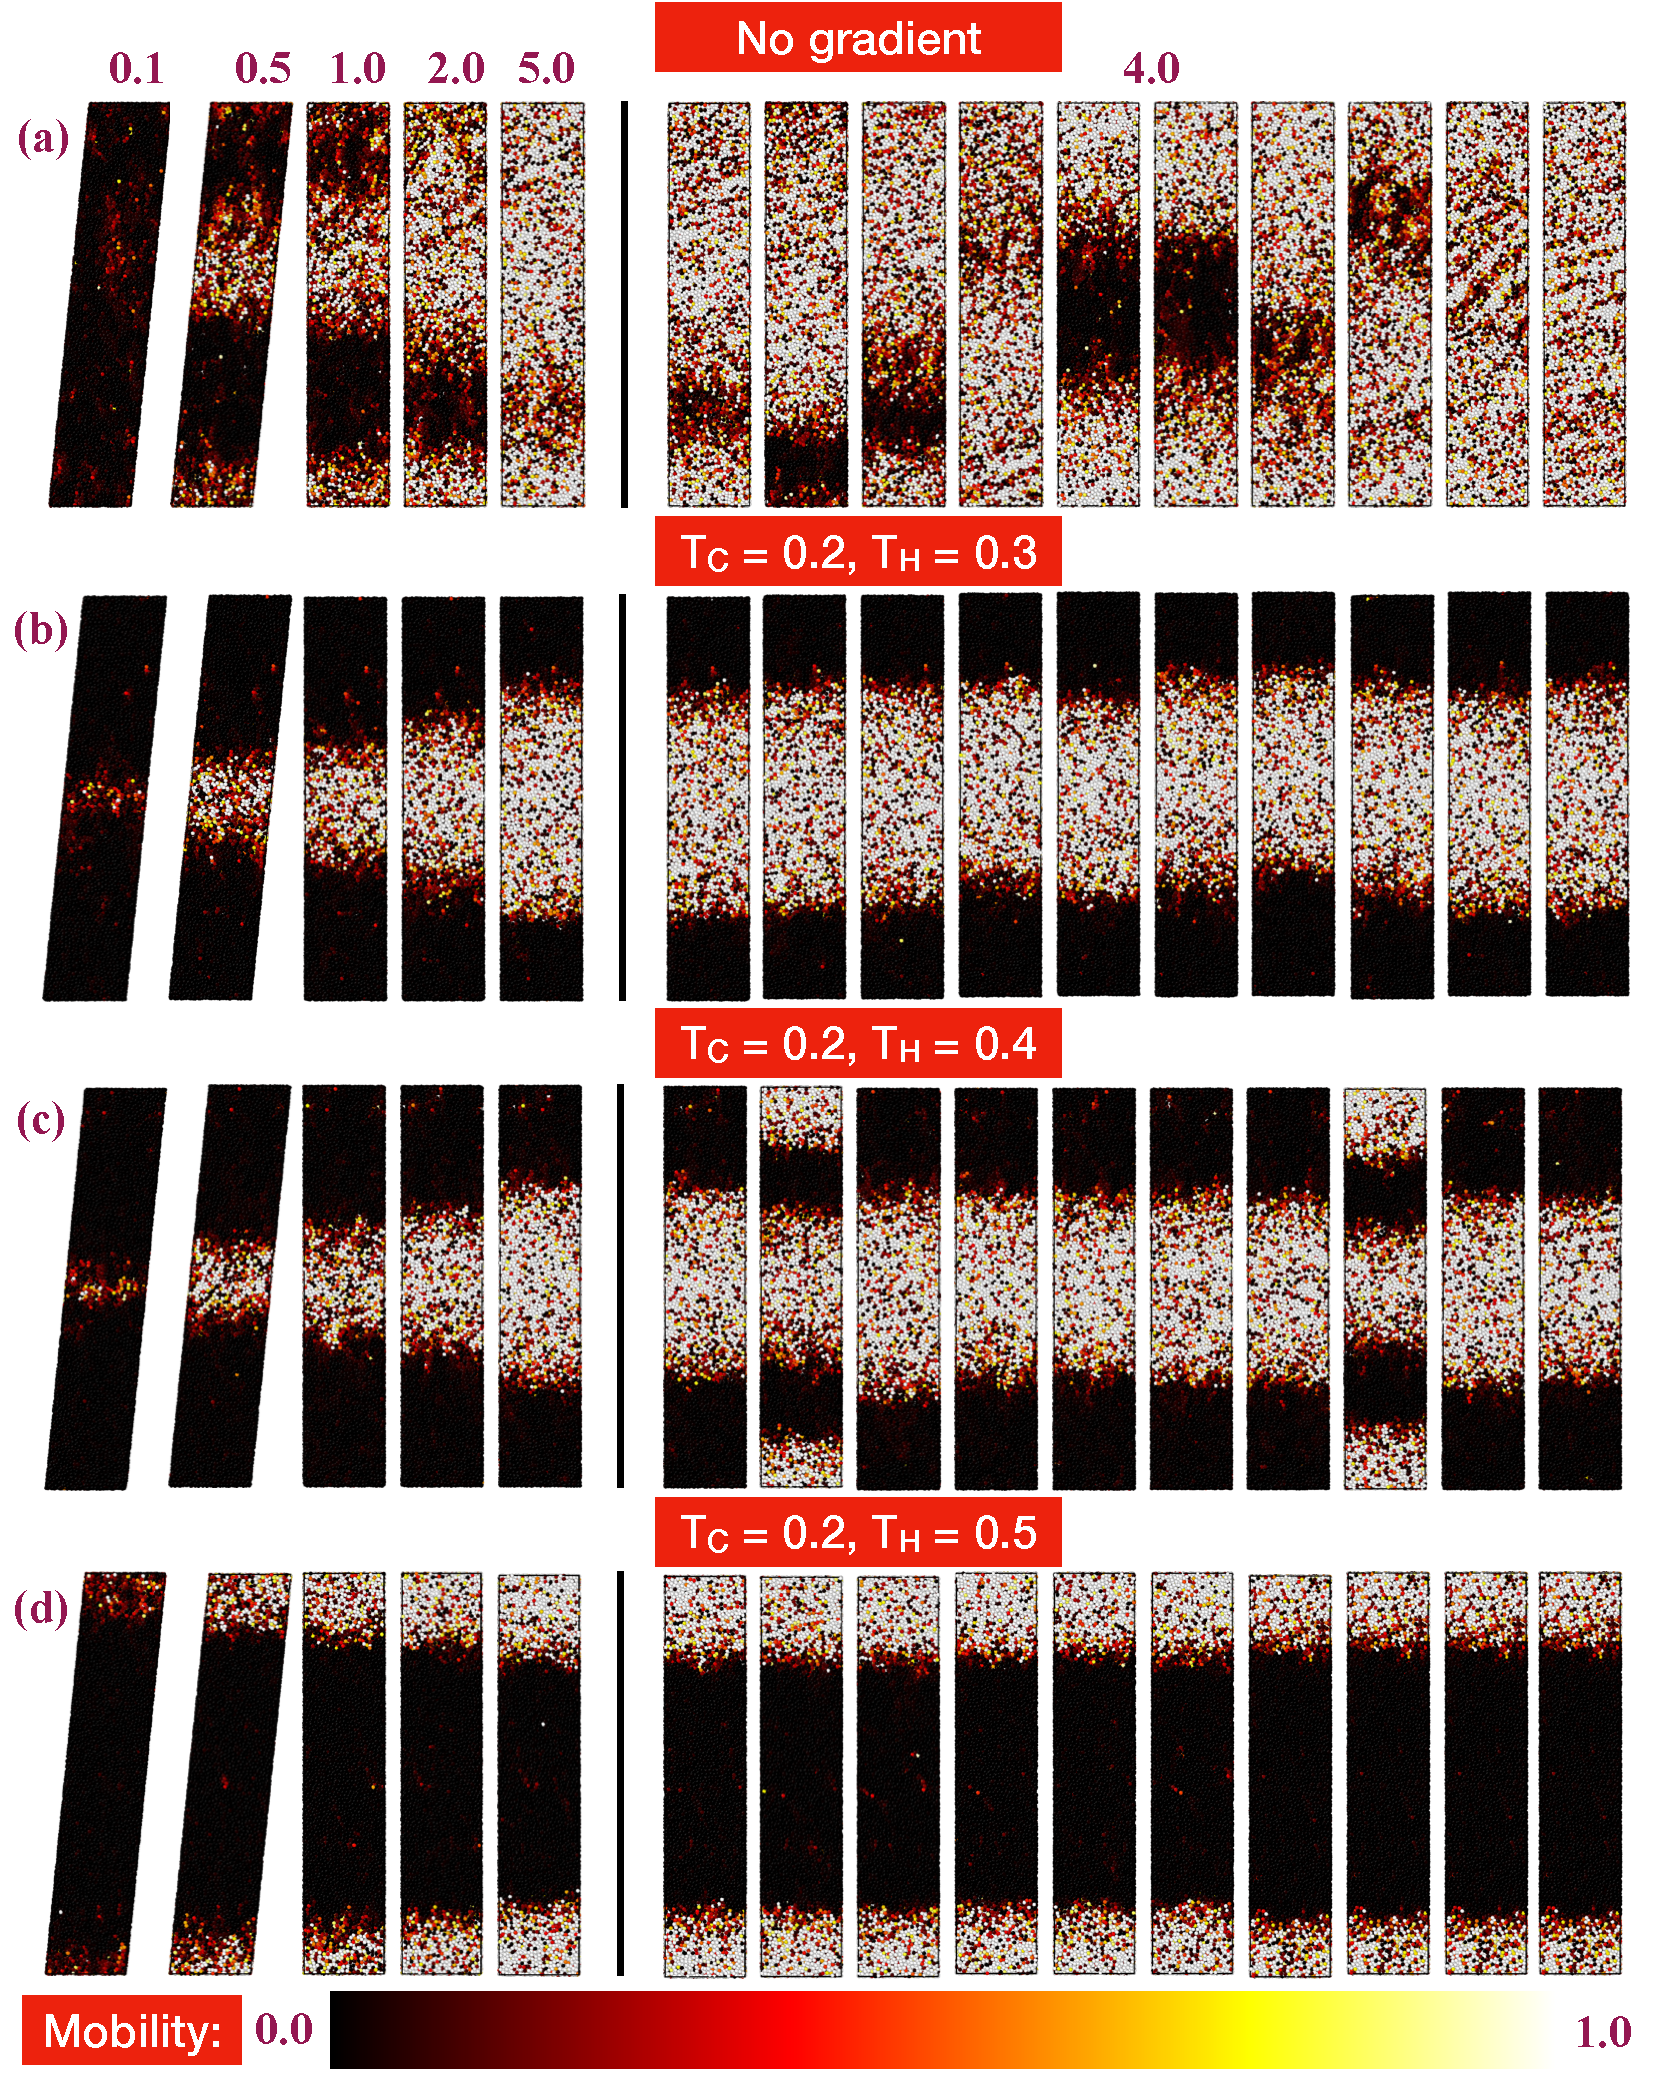
\includegraphics[width=13cm]{./figs/mobMap_tempGrad.pdf}
\caption[{\em Mobility maps of sheared thermally processed samples: impact of gradient}]{{\em Mobility maps of sheared thermally processed samples: impact of gradient.} Different temperature gradient pulses with $T_C = 0.20$ and $T_H = 0.30, 0.40, 0.50$ (also marked), are applied for $t_{\rm exp} = 2\times10^5$ to generate inhomogeneous glassy samples and then these samples are sheared with shear rate $\dot{\gamma} = 10^{-4}$. These maps are constructed using non-averaged single particle squared displacement in $z$-direction, assuming time at the start of the shear as origin. Upper panel (a) maps are shown for the case of unprocessed samples. Maps on the left side of the vertical line show the evolution of shear bands with strain $\gamma = 0.1, 0.5, 1.0, 2.0, 5.0$ (also marked), while maps on right side are shown at the fixed value of strain $\gamma = 4.0$ and starting with the same thermally processed sample but different random seed for DPD thermostat.}
\label{mapVaryGrad}
\end{figure}
%%%%%%%


In the previous section, we have analysed the macroscopic rheological response of inhomogeneous glassy samples. Now, we examine the inhomogeneous flow patterns at microscopic level of these samples, during the response to the applied shear. For this purpose, for a chosen initial state, we compute the mobility  maps using  single particle squared displacement $\delta r^2_z(t)$, measured with respect to the state at $t=0$, i.e. at the start of shear. These maps have been calculated at different strain values, using an imposed shear rate of $10^{-4}$; see Fig.~\ref{mapVaryGrad} and \ref{mapVaryExp}. The flow behaviour in terms of such mobility maps has been used in earlier studies \cite{golkia2020} to probe the emergence and evolution of the flow heterogeneities in the form of shear-bands. Here, we compare the flow patterns via the mobility maps, for both thermally processed and unprocessed samples.

In Fig.~\ref{mapVaryGrad}, we present the shear bands at the different strain values, for the untreated glassy samples (Fig.~\ref{mapVaryGrad}a) and  glassy samples treated via different temperature gradients ($T_C = 0.20 $ and $T_H = 0.30, 0.40, 0.50$) (Fig.~\ref{mapVaryGrad}(b-d)), as discussed above. On the left side of the vertical line in Fig.~\ref{mapVaryGrad}, shear bands have been shown at strain values $0.1, 0.5, 1.0, 2.0, 5.0$. In the unprocessed sample, at small strains, very weak shear band is formed from hot spots at random locations, and these gets spatially homogenized at a strain value of $4.0$. But inhomogeneous samples show very sharp localized band patterns, at early strain. The expansion of these shear bands become slower or the lifetime of shear bands become longer for bigger gradients, this can be observed visually by comparing the bands at a particular strain value for different thermal gradients. This observation is consistent with the macroscopic observations made above, viz. with the increase in spatial inhomogeneity in the gradient direction, the sample takes longer time for reach a spatially homogeneous steady state. We also note that for $T_H = 0.3, 0.4$, the band (faster region) nucleates in the middle of the sample, near the colder end, and it expands towards the hotter region, while for $T_H = 0.5$ the band nucleation happens near the hotter region and it expands towards the colder region. The difference in the location of the shearband formation could be due to relative local stability due to the spatial heterogeneity in the initial state.

Similarly, in Fig.~\ref{mapVaryExp}(a-d), we present the shear bands at the different strain values for the glassy samples treated using a fixed thermal gradient ($T_C = 0.2 $ and $T_H = 0.50$) but different exposure time $t_{\rm exp} = 0, 10^3, 10^4, 10^5$. In this case, the main observation is the lifetime of the band increases with the increase in the time window over which the initial states were exposed to the thermal gradient. This observation is consistent with the macroscopic measurements in Fig.~\ref{shear}d, where we observed that the timescale of reaching steady state increases with the increase in exposure time . The location of shear band is roughly the same in all cases of finite exposure time in Fig.~\ref{mapVaryExp}(b-d), similar to the case of Fig.~\ref{mapVaryGrad}d where the same gradient is applied for $t_{\rm exp} = 2\times10^5$ i.e., shear band always nucleates near the extreme ends close to hotter region.

%%%%%%%%%
\begin{figure}[hbt!]
\centering
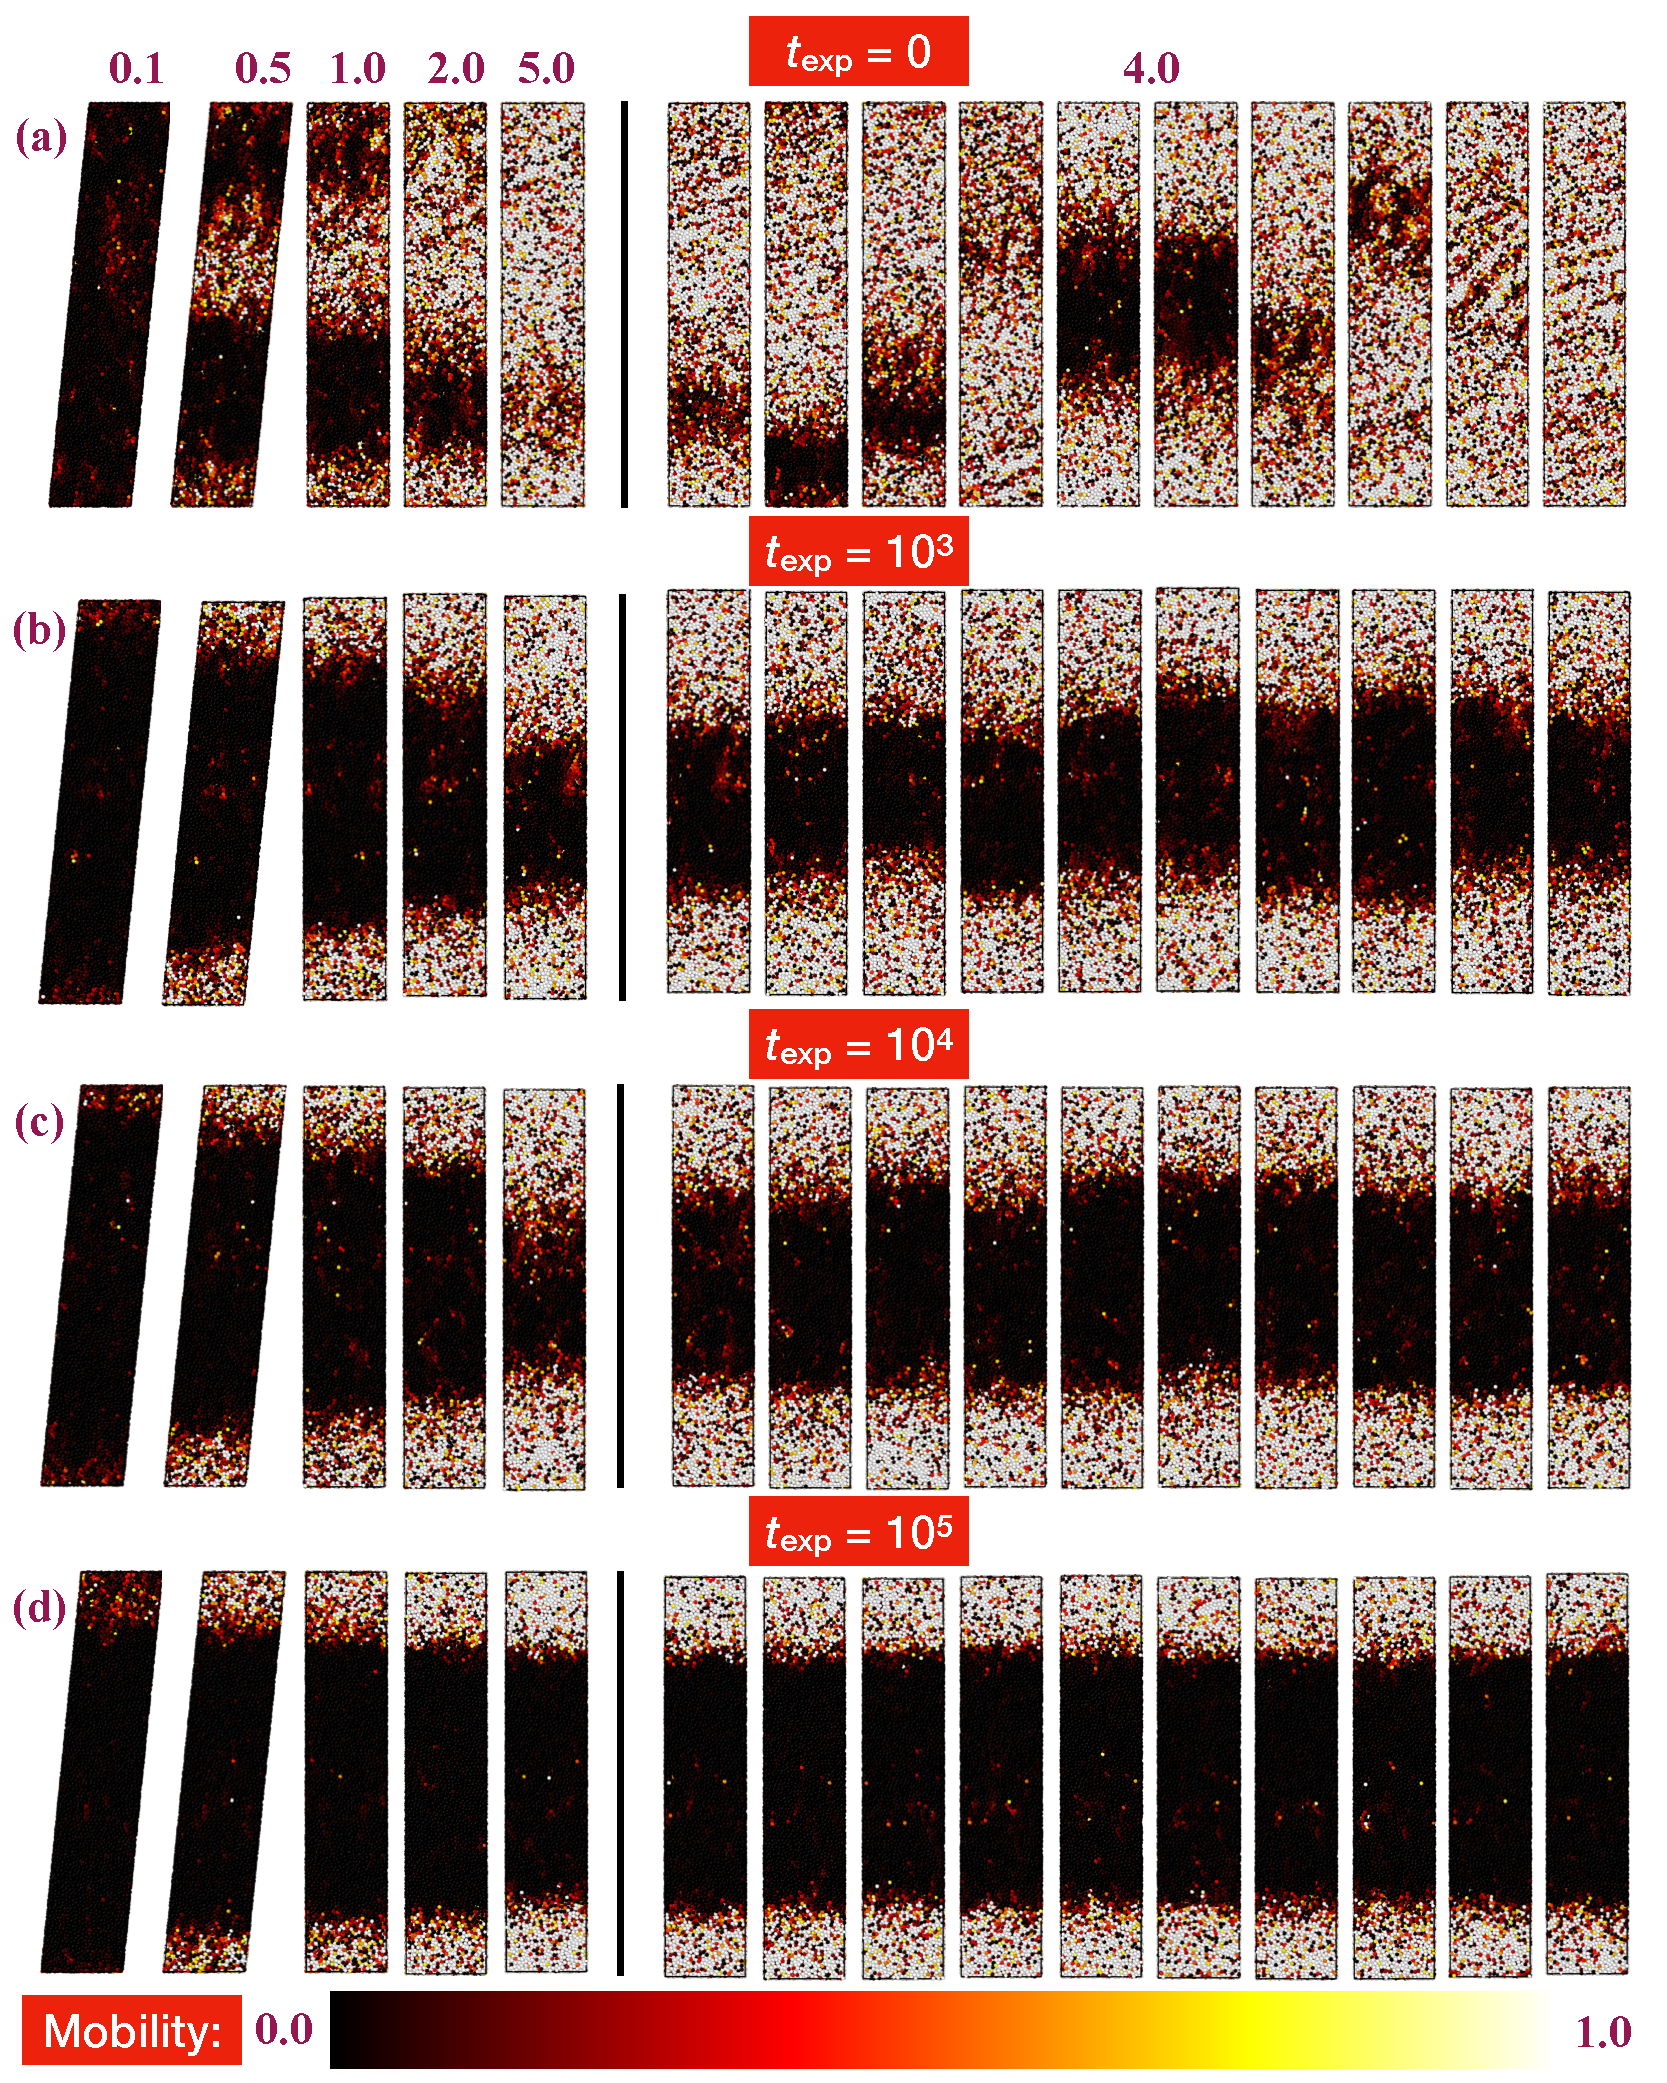
\includegraphics[width=13cm]{./figs/mobMap_tExp.pdf}
\caption[{\em Mobility maps of sheared thermally processed samples: impact of exposure time}]{{\em Mobility maps of sheared thermally processed samples: impact of exposure time.} A fixed temperature gradient pulse with $T_C = 0.20$ and $T_H = 0.50$ is applied for different duration $t_{\rm exp} = 0, 10^3, 10^4, 10^5$ (also marked) to generate inhomogeneous glassy samples and then these samples are sheared with shear rate $\dot{\gamma} = 10^{-4}$. These maps are constructed using using non-averaged single particle squared displacement in $z$-direction, assuming time at the start of the shear as origin. Upper panel (a) maps are shown for the case of unprocessed samples. Maps on the left side of the vertical line shows the evolution of shear bands with strain $\gamma = 0.1, 0.5, 1.0, 2.0, 5.0$ (also marked), while maps on right side are shown at the fixed value of strain $\gamma = 4.0$ and starting with the same thermally processed sample but different random seed for DPD thermostat.}
\label{mapVaryExp}
\end{figure}
%%%%%%%


%{\em Inhomogeneity decides the nucleation and growth of shear bands.} 
Finally, we demonstrate that the location of the density inhomogeneities in the initial sample, prior to shear, determines the location of the flow bands observed during the shear.
%Up to now we have seen the macroscopic and microscopic mechanism of failure is different in thermally processed inhomogeneous samples, compared with the glassy samples which are not exposed to any thermal gradient. In particular, we observed very special flow patterns in the shear response of these samples i.e., depending on the gradient used to treat the sample the shear band nucleation can be near the hotter region or colder region. Now, we want to understand the role of inhomogeneity in the determination of location of nucleation of shear band and its growth. 
For this purpose, we start with an inhomogeneous glassy sample obtained after switching off the gradient and perform at least $10$ different shear deformation simulations with $\dot{\gamma} = 10^{-4}$, using different random seed for the DPD thermostat which maintains the temperature at $0.2$. Hence, in each simulation, the spatial heterogeneity of the sample is same but the random kicks faced by particles during deformation are different. 
%Such analysis will help us in understanding the role of inhomogeneity in the determination of mode of failure. 
Next, we show on the right side of vertical line in Fig.~\ref{mapVaryGrad}, the mobility map at the strain value of $\gamma = 4.0$ for $10$ different simulations with same initial inhomogeneity at the start of deformation . In all samples, except for the case of a few samples at $T_H = 0.4$, mobility maps show similar  pattern, i.e., for $T_H = 0.3, 0.4$ shear band nucleates close to the colder region and expands towards the hotter region and for $T_H = 0.5$ shear band always nucleates near the hotter region at extreme ends and then expands towards the colder region. This is in contrast to the unprocessed sample where the slower regions are located at different levels along $z$, which is consistent with previous observations \cite{golkia2020}. Therefore, for the processed samples, we can conclude that there is no run-to-run variation, i.e. there is no stochastic effect is the selection of the location unlike the case of the unprocessed states \cite{golkia2020}. Hence, this selection of the location of shearband formation must be related to features in the initial structure. A similar exercise is also done for the case of samples having different exposure time; see right column of Fig.\ref{mapVaryExp}. There too we observe no run to run variation, specially for samples which have been exposed to the thermal gradient for long times. 

\section{Conclusions}

We have studied the shear response of inhomogeneous glassy samples prepared by exposing homogeneous glassy states to a thermal gradient pulse. Our aim is to understand whether the mechanical behaviour, specially the spatial response, is influenced by the initial structural heterogeneities. 


First, we have characterised the spatial inhomogeneity, generated via the thermal protocol discussed above, in terms of spatial profiles of density, concentration and local potential energy. We observe that the degree of heterogeneity is controlled by the applied thermal gradient and its exposure time. 

%We have investigated the failure mechanism in heterogeneous samples obtained by changing the thermal gradient for fixed exposure time and by changing the exposure time for a fixed gradient.

Next, the mechanical response was studied by driving these samples by a fixed shear-rate. We observe that the timescale at which the sheared inhomogeneous states achieve steady state is delayed, in comparison with the initial homogeneous glassy states, which is related to the slow flow homogenization within the samples. The microscopic insights of this failure mechanism in deformed inhomogeneous glassy samples is thereafter obtained via mobility maps. This analysis suggests that it is possible to have a control over the location of the failure via the initial spatial heterogeneity in the glassy state. In particular, location of shear band initiation has one-to-one correspondence with the heterogeneity in the sample, which is confirmed by a thought experiment involving the stochasticity of the thermostat vis-a-vis a single heterogeneous sample and showing that stochasticity has no role to play in the location of the shearband. 

The extension of this project should be to perform simulation studies at very low temperatures, where some interesting features are expected. Also, a computer experiment can be performed where different kinds of thermal pulses can be utilised to generate more variations in spatial heterogeneity aimed at targeted design. Further, other shear directions can be explored to understand the failure mechanism and its coupling to these heterogeneities.
\pagestyle{fancy}
\fancyhf{}
\renewcommand{\headrulewidth}{0pt}
\fancyfoot[C]{\leftmark}
\fancyhead[R]{\thepage}
\doublespacing
\chapter{Poiseuille flow of soft glass: role of thermalization protocol}\label{chap5}

\noindent\fbox{\parbox{\textwidth}
    {\color{myred}
    This chapter is based on the following publication \cite{vaibhav2021influence}:\\
    {\em Influence of thermalisation protocol on Poiseuille flow of confined soft glass}\\
    V. Vaibhav, and P. Chaudhuri, Physics of Fluids 33, 053103 (2021)}
}


\section{Introduction}

Soft glassy materials are all around us, both in nature and daily lives. In general, all glassy systems are characterised by the existence of a yield stress \cite{coussot2014yield, bonn2017yield, joshi2018yield}, i.e. a finite stress threshold needs to be overcome in order for the material to yield. For soft glasses (e.g. colloids, emulsions, gels, granular suspensions etc.), steady flow is observed once this yield threshold has been crossed, and this property has been utilised in diverse important applications. Prior to the onset of steady flow, fascinating spatio-temporal behaviour \cite{rodney2011modeling} is observed which are linked to the  occurrence of spatially correlated plastic events \cite{bocquet2009kinetic, nicolas2018deformation}, the cascade of which leads to yielding and flow. Such correlated processes continue in steady state and the bulk rheological flow curves are well described by the Herschel Bulkley function \cite{bonn2017yield}. Overall,
understanding and characterising the diverse rheological response \cite{bonn2017yield, joshi2018yield, tanner2018aspects, semwogerere2008shear, khabaz2021thermodynamics, jacob2019rheological, agarwal2019signatures, biswas2021quantifying, sriram2010active} of soft glassy materials has been actively undertaken to help in improving existing applications or design new materials with specific functions.

One of the possible ways to study the rheological response of soft glassy systems is via Poiseuille flow (check section-\ref{PoiseuilleFlow} of Chapter-\ref{chap1} for basic introduction to Poiseuille flow), which has become quite significant in the context of microfluidic devices \cite{tabeling2005introduction}, 3d printing \cite{zhu2019colloidal, nelson2020embedded} and also applications involving extrusion of materials \cite{ebendorff2007extrusion}, and therefore has been investigated via experiments \cite{goyon2008spatial, isa2009velocity, genovese2011crystallization, ballesta2012wall, nordstrom2010microfluidic}, numerical simulations \cite{chaudhuri2012dynamical, mansard2013molecular, pinaki2014, lulli2018metastability} and different coarse-grained models \cite{nicolas2013mesoscopic, papenkort2014channel, lulli2018metastability}. In the case of Poiseuille flow, the pressure gradient applied across the channel leads to the occurrence of a spatially non-uniform stress field across the width of the channel in the flow gradient plane. In the presence of an inhomogeneous stress field, the naive expectation is that  the material will flow, i.e. there will be finite shear-rate, wherever the local stress is above the yield stress. For Poiseuille flow, this would lead to blunted velocity profiles for soft glasses \cite{PhysRevE.77.011504} instead of the parabolic velocity profiles that occur for Newtonian fluids \cite{evansMorrissBook}. However, it was demonstrated that due to the interplay between the spatially correlated plasticity occurring in glassy systems, as discussed above, and the stress gradients that are characteristic to Poiseuille flow, there not only exists a macroscopic yield threshold that depends upon the channel width \cite{chaudhuri2012dynamical} but also the observed velocity profiles  deviate from those predicted from the Herschel-Bulkley bulk rheology, with the deviation increasing with decreasing channel width \cite{goyon2008spatial, mansard2013molecular}. Due to this fascinating non-local coupling, the onset of flow also takes place collectively across the channel, and hysteresis linked to metastable states are also observed in thermal systems \cite{pinaki2014, lulli2018metastability}.  Further, it has been demonstrated that due to such spatial correlations occurring during the flow, the rheological behaviour can be greatly influenced by the roughness of the confining walls of the channel \cite{mansard2014boundary}, which thus provides a design control for various applications. 


\section{Objective}

%In this work, we investigate a similar boundary driven effect, albeit in a different way. 
Previous studies \cite{baranyai1992isothermal} have demonstrated that in the presence of a spatially varying shear-rate, heat flow can occur even in the absence of any externally applied thermal gradient. Further, it was illustrated that for the case of Poiseuile flow of a fluid confined between walls via which temperature control is maintained, a spatially varying temperature profile emerges in steady state, which has a quartic spatial dependence as predicted from solutions of phenomenological hydrodynamic equations \cite{todd1995, varnik2002, binder2004molecular}. Motivated by this phenomenon, we investigate how such thermalised boundaries influence the Poiseuille flow of a model soft glass, both in steady state and also during the onset of flow from a quiescent state. We contrast our observations with the case where the confined fluid is thermalised directly, and not via the walls. Our main objective is to study the rheological response of a soft glass in the simultaneous presence of a local stress gradient (via the Poiseuille setup) and a local temperature gradient (via the temperature control using walls), and contrast that with the situation where the thermal gradient is absent during the Poiseuille flow. Thus, it is not a study of the efficacy of the two different kinds of thermostats, but rather investigating the rheological consequence of having non-uniform temperature within the channel during the Poiseuille flow. In the broader context, such a study is part of recent investigations into the role of dissipation processes \cite{nicolas2016effects, irani2019discontinuous, vasisht2018permanent} in determining the non-equilibrium response of sheared amorphous materials. 

%The paper is organised as follows. After the introductory note in Section I, in Section II, we discuss the model glass former that is studied, the method for setting up the Poiseuille flow for the glass confined between rough walls, and the methods for the two studied thermostats, viz. in one case, where the confined fluid is thermalised via the walls and another case, where the fluid is directly thermalised. In Section III, we discuss the results of our study, probing the behaviour in the quiescent state, and in the driven state, both in steady state as well as during the onset of flow. Further, we also discuss, in the same section, a brief comparison of response across varying channel widths. Finally, in section IV, we provide some concluding discussions.

                                                        
\section{Model and methods}

\subsection{The model glass former}

In this work, we consider the well-studied glass-forming model binary Lennard-Jones mixture \cite{Kob94} (check section-\ref{model} of Chapter-\ref{chap2} for more details about the model), whose rheological properties have been well characterized in terms of well-known soft glass phenomenology. 

All lengths are measured in the unit of $\sigma_{\rm AA}$, energy is expressed in the units of $\varepsilon_{\rm AA}$, the unit of time is $\sqrt{{m\sigma_{\rm AA}^{2}}/\epsilon_{\rm AA}}$ and that of stress is $\epsilon_{\rm AA}/ \sigma_{\rm AA}^{3}$. For this mixture,  the increase in relaxation timescales of the supercooled liquid with decreasing temperature can be fitted with mode coupling theory prediction, providing a mode-coupling critical temperature $T_{MCT} \approx 0.435$, below which conventional numerical simulations fail to obtain equilibrium dynamics. However, the putative glass transition temperature of the system, $T_{VFT} \approx 0.3$ is obtained by a Vogel-Fulcher-Tammam fit to the variation of relaxation timescale with temperature. We study the flow response of the mixture at $T_0=0.40$, which is in between  $T_{MCT}$ and $T_{VFT}$, i.e. within the thermal aging regime. We carry out extensive molecular dynamics simulations to study the response to external shear using  LAMMPS \cite{lammps}, with the equations of motion being integrated via velocity-Verlet scheme with time-step $\Delta t = 0.005$.

\subsection{Poiseuille flow}

For the purpose of studying channel flow, we initially consider a periodic rectangular box of dimension $L_x \times L_y \times L_z$, extended between $0$ to $L_x$ along $x$, $0$ to $L_y$ along $y$ and  $-L_z/2$ to $L_z/2$  along $z$. Different independent initial states are prepared by quenching well-equilibrated high temperature configurations at $T=5.0$  to $T=0.4$ below $T_{MCT}$, which are subsequently aged for a duration of $t_{age} = 10^4$. The particles in the two regions parallel to $xy$ plane for which $|z| > L_z/2 -3$ make the two amorphous walls (each of thickness $3 \sigma_{\rm AA}$) which confine the system to make a channel of width $L_z-6$. This construction of the walls is done after the aging process has been completed following the quench from $T=5.0$  to $T=0.4$. To implement Poiseuille flow, a force $F_x$ is applied on all the particles in the confined channel along $x$-direction \cite{todd1995pressure}. 


In this work, we study the Poisueille flow in channels of two different widths, viz. $w=100, 25$. For that purpose, we use two different sample sizes having roughly same number of fluid particles: $30 \times 30 \times 106$ (114 480 particles) and $120 \times 30 \times 31$ (133 920 particles), taking into account the confinement via walls. Most of the results are reported for channel $w=100$ and at the end, we provide a brief comparison with observations in $w=25$. The choice of the wider channel for the present study is led by the focus on investigating the role of thermal gradients in rheology, with smaller interference from effects due to confinement, which we will also briefly probe as indicated. All reported results are averaged over 10-30 independent trajectories.


%%%%%%%
\begin{figure}
\centering
\includegraphics[width=15cm]{figs/schematicPoiseFlow.pdf}
\caption[{\em Schematic of Poiseuille flow geometry and snapshots of the binary LJ mixture confined between rough walls for two different channel widths}]{Schematic of flow geometry. Snapshots of the binary LJ mixture, confined between rough walls along the $z$ direction, is shown for (a) wide [$w=100$] and (b) narrow [$w=25$] channels. The external forcing which generates the Poiseuille flow is along the $+x$-direction, as marked in (c), and the shear thus develops in the $xz$ plane, with the resultant shear stress profile schematically illustrated in (c). Also shown schematically in (c) are the expected velocity profiles for a Newtonian and a yield stress fluid, which respectively correspond to parabolic or blunt profiles.}
\label{fig0}
\end{figure}
%%%%%%%

\subsection{Couette flow}

We also compare some results of the Poiseuille flow with those of the Couette flow, where the shear is imposed by fixing the shear-rate, corresponding to which a uniform shear stress is maintained. The Couette flow simulations are done for $N=8000$ particles in a cubic box with periodic boundary conditions in all three directions and the fixed shear-rate is imposed by deforming the box at the corresponding rate \cite{PhysRevE.102.023002} and simultaneously integrating the equations of motion of the particles. The required ambient temperature is maintained via a DPD thermostat (check section-\ref{thermostat} of Chapter-\ref{chap2} for more details about DPD thermostat) \cite{shrivastav2016yielding}.

\subsection{Implementation of thermostats}

The applied forcing to maintain Poisuille flow also leads to the generation of heat. If a thermostatting mechanism removes the excess heat generated, then a steady state is achieved where rate of heat generation becomes equal to the rate of heat removal. In this stage, a steady profile of different quantities like temperature, velocity of flowing particles, stress etc is maintained. Different thermostatting procedures have been adopted in various studies related to flow in confined channels \cite{hartkamp2017,luding2007,yethiraj1997}. In this study, we will consider two such thermalisation procedures and study how the flow of a glass forming material is influenced by the nature of the thermostat.

For the construction of the thermostats, we consider two kinds of confining walls: first is the \textit{vibrating wall}  and second is the \textit{frozen wall}: (i) In the case of vibrating wall, particles are tethered to their initial positions (at $t_{age} = 10^4$) and at each time-step, experiences a harmonic force equal to $-\kappa r$, where $\kappa$ is the spring constant and $r$ is the displacement of the particle with respect to initial position \cite{thompson1990,powles1992,todd1995,evansMorrissBook,koplik2001,varnik2002,koplik2006}. Such a wall consisting of vibrating particles does not allow the confining particles to escape. The wall particles keep interacting among each other and  with the confining fluid in the channel, resulting into continuous exchange of momentum and energy between wall and fluid particles. Further, each of the walls consists of three different layers (each of thickness unity) and the velocities of the particles in each layer is separately rescaled to the target temperature $T = 0.4$ at each time-step\cite{kim2008}. Fluid particles in the channel are not coupled to any separate thermostat, their dynamics is solely influenced by the two walls. This mechanism is able the maintain a constant temperature in the channel in the absence of any external forcing, as we will demonstrate below. Also, the dynamics of the fluid particles is not perturbed because of any coupling to external heat bath, making this probably the most natural way to remove the excess heat generated in the system, closely mimicking the experimental conditions. In the discussion below, we will refer to this thermostatting process as the "wall thermostat".
(ii) In the case of second type of wall, particles building the wall are frozen at their respective positions at $t_{age} = 10^4$  by setting their velocity to zero and fixing the forces acting to zero\cite{pinaki2014}. The temperature of the  fluid particles is maintained at a certain temperature via a DPD thermostat (using dissipation constant unity)\cite{dpd}, which does not introduce any bias in the spatial profiles of the emergent flow (check section-\ref{thermostat} of Chapter-\ref{chap2} for more details about DPD thermostat). Henceforth we will refer to this thermostat condition as the "DPD thermostat".


\section{Results}

\subsection{In the absence of shear}

We first compare the structural and thermal state inside the channel, in the absence of external forcing, for the two thermostatting methods.  The corresponding data is shown in Fig.\ref{fig1}.  As expected, in both cases, the temperature profile $T(z)$ is identical across the channel; see  Fig.\ref{fig1} left panel. However, there is a difference, as visible from the temperature profiles. For the wall thermostat, the wall temperature is maintained at $T=0.40$, whereas for the DPD thermostat, the wall temperature is zero since the particles constituting the wall are completely frozen. Next, for the two thermostat conditions, we examine the density profile $\rho(z)$ and observe that the structure is also the same across the channel; the local density fluctuates around the mean density of 1.2 as can be seen in  Fig.\ref{fig1} right panel.  Hence, in the absence of any external drive, the two thermostats provide similar thermal and structural conditions.
%%%%%%%
\begin{figure}
\centering
\includegraphics[width=15cm]{figs/compThermostat.pdf}
\caption[{\em Temperature and density profiles in the absence of flow}]{In the absence of flow, comparison of temperature $T(z)$ (left) and density profiles $\rho(z)$ (right), for the two thermostats as labelled.}
\label{fig1}
\end{figure}
%%%%%%%

Note that for computing these spatial profiles as well other profiles to be discussed later, we have subdivided the $z$-direction into layers of thickness $dz = 1$ parallel to $xy$-plane and averaged the data along $x$ and $y$ directions within each such layer, to obtain the spatial profiles that we report.


\subsection{In the presence of shear: steady state}

First, we address the important question of how do the temperature profiles look like inside the channel, in steady state Poiseuille flow, for different applied external forcing. This is shown in Fig.\ref{fig3}. For the case of DPD thermostat, there is no difference in $T(z)$ with increasing magnitude of forcing, within the range explored -- it is spatially uniform across the channel; see right panel of Fig.\ref{fig3}. On the other hand, for the case of wall thermostats, the temperature across the channel not only varies, with a maximum at the centre of the channel, but also this maximum value is dependent on the external forcing -- the larger the forcing, the larger is the local temperature; see left panel of Fig.\ref{fig3}. Due to this non-uniform thermal conditions, some  regions even have local temperature above $T_{MCT}$, i.e. those regions are in the supercooled state and therefore should impact the rheological behaviour of the system. Note that, in the case of both thermostats, for computing the temperature profiles accurately via the local kinetic energies, we subtract the local mean streaming velocity and thereby use the instantaneous velocity fluctuation in the flow direction \cite{todd1995}. For Newtonian fluids, the temperature profile is described by the following function \cite{todd1995, binder2004molecular}: $T(z)=T_0 + A(\rho_0{F_x}w^2)^2[1-(2z/w)^4]$, where $A$ is dependent on the thermal conductivity and the viscosity of the fluid (check section-\ref{PoiseuilleFlow} for the derivation of this expression for temperature profile). We check whether such a quartic function can fit the temperature profiles that we observe, which are shown in the left panel of Fig.\ref{fig3}, and note that the fits do not work. One of the reasons is that the fluid is not Newtonian, rather a yield stress fluid implying that the viscosity depends upon shear-rate and thus the above function does not provide a good description.

%%%%%%%
\begin{figure}
\centering
\includegraphics[width=15cm]{figs/tempComb.pdf}
\caption[{\em During Poiseuille flow, comparison of temperature profiles within the channel, in the presence of the two thermostats}]{During Poiseuille flow, comparison of temperature profiles within the channel, in the presence of the two thermostats, viz. wall thermostat (left) and DPD thermostat (right), for different strengths of the applied force (marked).  Also shown in the left panel, with dashed lines, are fits using the function $T(z)=T_0 + A(\rho_0{F_x}w^2)^2[1-(2z/w)^4]$, where A is a fit parameter.}
\label{fig3}
\end{figure}
%%%%%%%

%%%%%%%
\begin{figure}[htb!]
\centering
\includegraphics[width=15cm]{figs/denStress.pdf}
\caption[{\em Comparison of density and stress profiles in the presence of the two thermostats}]{Poiseuille flow. (Top) Comparison of  density profile, $\rho(z)$ in the presence of the two thermostats, viz. wall thermostat (left) and DPD thermostat (right), for different strengths of the applied force (marked). (Bottom) the shear stress profile emerging in the channel, for different strengths of the applied force (marked), in the presence of the two thermostats, viz. wall thermostat (left) and DPD thermostat (right). Also marked using dashed lines, in both left and right panels, is the bulk shear stress yield threshold ($\sigma_d=0.242$) at temperature $T=0.4$.}
\label{fig2}
\end{figure}
%%%%%%%

Having clarified the ambient thermal conditions, we analyse how the density profiles change when the external forcing is introduced in the form of Poiseuille flow. Here, we discuss the situation when the non-equilibrium steady state has been attained, for both thermostats, after application of the external force. The nearly flat density profile observed in the quiescent case is modified and there is some variation across the channel with a mild maximum at the centre of the channel; see Fig.\ref{fig2} top panel. The shape of the density profiles seems to be roughly similar for both the thermostats that we have studied. In general, such spatial variation hints at shear-induced migration effects, which we will discuss later.

We have then computed the shear-stress profiles building up inside the channel, as we vary the external forcing, using the standard Irving-Kirkwood expression \cite{todd1995pressure}. The corresponding data is shown in Fig.\ref{fig2} bottom panel. The shear stress profiles for both thermostats are identical and has the spatially linear profile, as is expected from mechanical stability \cite{todd1995pressure}. We also mark on the plots the bulk yield stress value ($\sigma_d \approx 0.24$) estimated from Couette flow measurements at the same temperature ($T=0.4$). We note that the naive expectation is that for each applied forcing, the spatial regions having local stress between $\{-\sigma_d, \sigma_d\}$ would see no flow, i.e. the local shear-rate should be zero. We analyse this aspect, further, below.

Hence, the different local thermal conditions for the two different thermostats do not affect the structural properties and thus the shear stress field that is set up. 


%%%%%%%
\begin{figure}
\centering
\includegraphics[width=15cm]{figs/velVelGrad.pdf}
\caption[{\em Steady state velocity profiles and corresponding spatial profile of local shear-rates for the different strengths of the applied force, for the two thermostats}]{Poiseuille flow. Steady state velocity profiles (top) and corresponding spatial profile of local shear-rates (bottom), for the different strengths of the applied force (marked), and for the two thermostats, viz. wall thermostat (left) and DPD thermostat (right) In the right panel, the zones within each pair of vertical dashed lines (having same color) correspond to the region where the local shear stress is below the bulk yield threshold at $T=0.40$ for each external forcing (same colored lines). The arrows in the top right panel indicate the direction of increasing $F_x$ for the sequence of vertical dashed lines.}
\label{velocityprofiles}
\end{figure}
%%%%%%%



Now, we address the important question whether the rheological response differs under these contrasting thermal conditions. The first check is via the velocity profiles observed in steady state, in the case of the two thermostats. As can be seen in the top panel of Fig.\ref{velocityprofiles}, the shape of the velocity profiles is consistent with what is observed for Poiseuille flow of soft glassy materials in wide channels. Unlike the parabolic flow of Newtonian fluids, here we observe blunted profiles due to the underlying Herschel-Bulkley shape of rheological curves, which we will further discuss below.  Consequently, the spatial profile of local shear-rates has a non-linear shape, compared to the linear shape expected for Newtonian fluids; see bottom panel of Fig.\ref{velocityprofiles}. At the centre of the channel, it should be noted that the local shear-rate is not zero as should be the case for yield-stress fluids, but seems to have a finite value \cite{mansard2013molecular}. However, the local shear-rate signal is very noisy at the centre of the channel and it is difficult to ascertain any differences with changing magnitude of the external forcing. Note that simple fluidity models \cite{goyon2008spatial, chaudhuri2012dynamical} predict finite shear-rates in regions where the local stress is less than the bulk yield stress, via non-local effects \cite{bocquet2009kinetic} due to the interplay of elasto-plastic correlations intrinsic to glassy systems and the imposed stress gradient via the Poisuielle flow; but, this effect becomes weaker with increasing width of the channel.

When we compare the response to the same external forcing (e.g. $F_x=0.010$), for the case of the two thermalisation protocols, we first note that in the centre of the channel, where the profiles are blunted, the velocity is larger in the case of the wall thermostat than the DPD thermostat. Further, the central blunt region is also more narrow for the case of the wall thermostat, the curvature also changes and consequently the local shear-rate is higher at any region away from the centre of the channel. These are consequences of the existence of local thermal gradient as well as higher local temperature in that region, for the case of temperature control via the walls. 

At any fixed forcing $F_x$, the deviation in local temperature $T(z) - T_0$ scales with $F_x^2$, as derived for Newtonian fluids. Thus, with increasing $F_x$, there are larger local temperatures which implies larger shear-rates compared to the case of spatially uniform temperatures, and hence larger deviations in local velocity.

Note that in all cases, no slip is observed in the velocity profiles due to the choice of rough boundaries. Further, note that the non-monotonicity in the local-shear profiles occur where the amorphous boundaries begin, i.e. where the flow velocity becomes negligibly small.

%%%%%%%
\begin{figure}
\centering
\includegraphics[width=15cm]{figs/stressStrain.pdf}
\caption[{\em Comparison of local flow curves for the different strengths of the applied force, corresponding to the two thermostats}]{Comparison of local flow curves, i.e. local stress vs local strain-rate, for the different strengths of the applied force (marked), corresponding to the two thermostats, viz. wall thermostat (left) and DPD thermostat (right). Also shown in the right panel, using a dotted line, is a Herschel-Bulkley fit to the collapsed data using $\sigma = \sigma_0 + K\dot{\gamma}^n$ with $\sigma_0 = 0.205$, $K = 2.188$ and $n = 0.328$.}
\label{localflow}
\end{figure}
%%%%%%%

%%%%%%%
\begin{figure}
\centering
\includegraphics[width=15cm]{figs/stressStrain_0p41.pdf}
\caption[{\em Comparison with bulk rheology data obtained from Couette flow}]{Comparison with bulk rheology data obtained from Couette flow. (Left) Variation of stress with shear-rate during Couette flow at $T=0.40, 0.41$ (in lines, as marked), shown along with local stress vs local shear-rate data (in symbols) where local temperature is in the range $[0.405,0.415]$ obtained from Poiseuille flow with wall thermostat. (Right) Variation of stress with shear-rate during Couette flow at $T=0.40$, shown along with the aggregated data for Poiseuille flow using DPD thermostat and the corresponding Herschel-Bulkley fit [see Fig.\ref{localflow}].}
\label{couettecompare}
\end{figure}
%%%%%%%

Next, to analyse the rheological response in greater detail, we probe the dependence of local shear-rate on local stress. For each applied $F_x$, we know the spatial dependence of shear stress (see bottom panel of Fig.\ref{fig2}) and also the spatial dependence of the shear-rate (see bottom panel of Fig.\ref{velocityprofiles}). Hence, at each spatial location, we have information on how local shear-rate depends upon local shear stress. This, we can aggregate for the different magnitudes of external forcing, and then plot local shear-rate vs local stress, which is shown in Fig.\ref{localflow} for the two thermostats. For the case of DPD thermostat, the data for different imposed $F_x$ values collapse into a single master curve; there is some scatter at small local shear-rates which is due to the noisiness of the data at the centre of the channel. This collapsed data can be fitted by the Herschel-Bulkley form $\sigma = \sigma_0 + K\dot{\gamma}^n$ with $\sigma_0 = 0.205$, $K = 2.188$ and $n = 0.328$ as the fit parameters. On the other hand, for the wall thermostat, no such data collapse occurs; rather, there seems to be distinct branches for each $F_x$.

Further, we can verify how these local flow curves constructed from the Poiseuille flow data for the local stress vs local shear-rates compare with the bulk rheology data obtained from Couette flow studies using periodic boundary conditions. Note that the shear stress is spatially homogeneous for the Couette flow, while it is inhomogeneous for the Poiseuille flow.The Couette flow simulations are done for imposed constant shear-rate. This imposed shear develops shear stress within the system, and the variation of the macroscopic shear-stress with the imposed shear-rate, constitutes the bulk rheological flow curve \cite{bonn2017yield}. This is in contrast to the local shear stress vs local shear-rate measurements that we are doing for the Poiseuille flow. The naive expectation is that for a wide enough channel, the local flow curve measured for Poisuielle flow would converge to the bulk flow curve, since it would ideally be a unique material property of the model system independent of rheological protocol. However, as has been demonstrated before \cite{goyon2008spatial, chaudhuri2012dynamical} , deviations are observed for a narrow channel, due to enhanced non-local effects occurring via the interplay between the inhomogeneous stress field and the intrinsic plastic correlations within a glassy system \cite{bocquet2009kinetic}.

First, we make the comparison between the bulk and local flow curves for the case of the DPD thermostat, where the temperature across the channel is maintained at the target temperature of 0.40; see right panel of Fig.\ref{localflow}. If we compare with the flow curve obtained from Couette flow, we see that there is some deviation, which is known to occur due to the non-local effects in channel flow as discussed above; even for channels as wide as 100 diameters, such effects cannot be ruled out. For the case of the wall thermostat, doing this comparison is non-trivial since the local temperature is also varying [see left panel of Fig.\ref{fig1}]. So, to do a first comparison between local and bulk flow data for this situation, we select one specific temperature value, viz. $T=0.41$. To obtain the data from Poiseuille flow, where there is a scatter of local temperatures around $T=0.41$, we consider cases where the the  local temperature is in the range of $[0.405,0.415]$ and for those zones, we collect the data for local stress and local shear-rate.  This is then compared with the Couette flow data computed for temperature $T=0.41$; see left panel of Fig.\ref{localflow}. We observe a large deviation -- at any particular local stress, the flowing glass has a larger shear-rate. Hence, it is evident that just by knowing the local temperature, it is not possible to predict the flow behaviour. Rather, there is enhanced plasticity as captured via the increase in local shear-rates, which would imply that the existence of both a stress gradient and temperature gradient significantly affects the rheology.

%%%%%%%
\begin{figure}[t]
\centering
\includegraphics[width=15cm]{figs/denShrRt.pdf}
\caption[{\em Steady state variation in local density fluctuations with local shear-rate for wall thermostat and DPD thermostat}]{Steady state variation in local density fluctuations, $\rho_z-\rho_0$, with local shear-rate in the case of wall thermostat (left) DPD thermostat (right), characterising particle migration occurring due to shear.}
\label{migration}
\end{figure}
%%%%%%%

We observe that there is increasing decrease in local density with increasing local shear-rate and also an enrichment at lower shear-rates, which are consistent with previous observations. All these effects are more pronounced with increasing $F_x$. However, we note that the deviations are around $1\%$ for the largest forcing that we have studied. Further the effect seems slightly weaker in the presence of thermal gradients, i.e. for the wall thermostat. The presence of thermal current from the wall towards the centre, due to the thermal gradient, could be a counterbalancing factor, which needs further probing.



\subsection{In the presence of shear: transient behaviour}

%%%%%%%
\begin{figure*}
\centering
\includegraphics[width=15cm]{figs/vcmx.pdf}
\caption[{\em Transient Poiseuille flow: time evolution of mean flow velocity}]{Transient Poiseuille flow. Time evolution of mean flow velocity $v_{cm_x}$ from quiescence to steady-state for different applied $F_x$ as marked, for wall thermostat (left) and DPD thermostat (middle). (Right) Variation of the corresponding  timescale for onset of steady state $\tau_0$ for different magnitudes for external drive characterised by the wall stress $\sigma_w=\rho{F_x}w/2$, for the two thermalisation conditions.}
\label{onset}
\end{figure*}
%%%%%%%

%%%%%%%
\begin{figure}
\centering
\includegraphics[width=15cm]{figs/profDev.pdf}
\caption[{\em Transient Poiseuille flow: development of spatial profiles of temperature, velocity and shear-rate, for the wall thermostat and DPD thermostat}]{Transient Poiseuille flow. Development of spatial profiles of temperature (top), velocity (middle) and shear rate (bottom), with time (as indicated) after imposition of a forcing $F_x = 0.010$; left panel corresponds to the wall thermostat and the right panel corresponds to the DPD thermostat. For each observation time, data has been averaged over a period of $\delta t = 250$ around the indicated time. Solid line is the steady state behaviour that is eventually observed.
}
\label{onset2}
\end{figure}
%%%%%%%


Having analysed the steady state flow behaviour, we now investigate the way to steady state from the initial quiescence, after the imposition of the external forcing. This can be studied by monitoring the mean flow velocity in the direction of flow \cite{pinaki2014}, $v_{cm_x}$, for the different applied $F_x$, and this is shown in the left and middle panels of Fig.\ref{onset} for the wall thermostat and DPD thermostat conditions, respectively. In the absence of the external drive, the average flow velocity is of course zero. When the external drive is switched on, $v_{cm_x}$ increases over a certain time window and eventually settles to a finite steady value, which increased with increased forcing. Further, as discussed above, we note that the steady state value of $v_{cm_x}$ is larger under wall thermostat conditions, for a fixed magnitude of the external forcing, implying that the flow is faster. We can study this further by focusing on the time evolution of the spatial profiles of velocity and temperature, for the same fixed force, but different thermostats, which we illustrate in Fig.\ref{onset2}. In the top panel, we show the time evolution of the temperature profile $T(z)$. For the DPD thermostat, the local temperature is always at the set value of 0.4. On the other hand, for the wall thermostat, $T(z)$ induced by the external force, emerges with time, before reaching the steady state profile.  Next, if we focus on the velocity profiles, shown in the bottom panel of  Fig.\ref{onset2}, we see that these also gradually evolve with time, for both thermostats, as expected. However, as can be easily seen, this is faster for the wall thermostat and the changes are happening as the local temperature also evolves towards steady state. Hence, the emergence of flow and thermal conditions are interlinked in this case.

Next, for each value of $F_x$ and for both the thermostat conditions. we estimate the timescale for the onset of steady state, $\tau_0$, by measuring when $v_{cm_x}(t)$ reaches the terminal steady state value. In the right panel of Fig.\ref{onset}, we show the variation of $\tau_0$ with each forcing characterised by the wall stress $\sigma_w=\rho{F_x}w/2$. First, we note that as expected \cite{pinaki2014}, the timescale for the onset of steady flow increases with decreasing $\sigma_w$. Further, we also note that for any particular $\sigma_w$, $\tau_0$ is larger in the presence of the DPD thermostat than the wall thermostat; the faster flow leads to faster onset of steady state. One can also then expect that the threshold in  $\sigma_w$, i.e. where $\tau_0$ is predicted to diverge, decreases for the case of the wall thermostat due to the presence of the thermal gradient.



%%%%%%
\begin{figure}
\centering
\includegraphics[width=15cm]{figs/cw1.pdf}
\caption[{\em Comparison of response for wide $w=100$ and narrow $w=25$ channels: spatial profiles of temperature, density, shear stress}]{Comparison of response for wide $w=100$ and narrow $w=25$ channels. Spatial profiles of temperature (top), density (middle), shear stress (bottom). In each case, left panel is data
for wall thermostat and right panel is for DPD thermostat. Note that $\tilde{z}$ corresponds to the scaled distance $\tilde{z}=2z/w$.}
\label{narrow1}
\end{figure}
%%%%%%%

\subsection{In the presence of shear: changing channel width}

We have also done some studies for a narrower channel ($w=25$), and we compare the observations with that for $w=100$ for a couple of wall stress values, viz. $\sigma_w=0.60, 0.66$, which provides the correct scale for comparing across different channel widths \cite{mansard2013molecular}.

First, if we compare the obtained temperature profiles in the case of wall thermostat, as shown in the top panel of Fig.\ref{narrow1}, the maximum temperatures observed are much less in the narrower channel. We recall that $T(z) - T_0 \propto \sigma_w^2w^2$, implying that narrower channels will witness lower temperatures for the same $\sigma_w$ even though the non-uniformity is still there. 

The density profiles, shown in the middle panel of Fig.\ref{narrow1}, exhibit oscillations due to layering effects for the narrow channel and this oscillations seems more pronounced for the DPD thermostat since the wall particles are static in that case. The shear stress profiles, shown in the bottom panel of  Fig.\ref{narrow1}, reveal deviations from the expected linear spatial profiles, which is related to the density oscillations with increasing confinement.


%%%%%%%
\begin{figure}
\centering
\includegraphics[width=15cm]{figs/cw2.pdf}
\caption[{\em Comparison of response for wide $w=100$ and narrow $w=25$ channels: spatial profiles of velocity and shear rate}]{Comparison of response for wide $w=100$ and narrow $w=25$ channels. Spatial profiles of  velocity (top), shear-rate (bottom). In each case, left panel is data
for wall thermostat and right panel is for DPD thermostat. Note that $\tilde{z}$ corresponds to the scaled distance $\tilde{z}=2z/w$.}
\label{narrow2}
\end{figure}
%%%%%%%

Next, we focus on the flow properties, viz. the local shear-rate profiles that are set up as shown in the bottom panel of Fig.\ref{narrow2}. In the case of DPD thermostat, decreasing channel width leads to increased curvature of the velocity profiles at the centre of the channel and thus increased local shear-rates, as observed in the right panel of Fig.\ref{narrow2}. This is a known consequence of the enhanced non-local effects with increasing confinement \cite{goyon2008spatial, mansard2013molecular}. 

However, for the case of the wall thermostat, the effect seems more complicated, due to the additional interplay with the non-uniform thermal conditions. For the smaller $\sigma_w$, if we compare the responses within the wide and the narrow channel,  the local shear-rates do get enhanced for the narrower channel; see left bottom panel of Fig.\ref{narrow2}. However, this is not the case for the higher $\sigma_w$, where the local shear-rates at the central region of both the wide and narrow channels seems comparable. One can understand this in the following way. There are two competing sources for enhancing local plasticity, one the increasing stress gradient and the other the thermal gradient. In the case of the wide channel, the thermal gradient is larger, whereas for the narrower channel, the stress gradient is larger. It seems that these competing effects get compensated leading to comparable rheological response in the central region for the two channel widths.  However, we also note that if we compare the response in the narrow channel for the DPD and the wall thermostat, the local shear-rates are higher in the latter case, implying that the thermal gradient, however small, does play its role in enhancing local plasticity.

Thus, this analysis gives us a glimpse into the complex interplay between the different existing gradients, viz. thermal and shear stress, and the correlated plastic processes intrinsic to glassy systems, which need further investigation.

\section{Conclusions}

In this work, we have studied the Poiseuille flow of a model soft glass, using two different thermalisation protocols. In one case, the confined material is thermalised via the walls, which are kept at the target temperature. Such a thermostatting procedure seems close to several practical applications where temperature control is easier to maintain via the confining walls, e.g. a complex fluid confined between hot or cold walls. In the other case, we thermalise the fluid directly and the particles constituting the walls remain completely frozen. Such a thermalisation procedure is also possible in diverse applications. The temperature targeted for thermalising is below the mode coupling temperature, but above the glass transition temperature, and thus in the ageing regime. In both cases, the walls are amorphous in nature, with the structure matching that of the confined aged glass. We emphasise that our objective is to study the rheological response of the confined glass under these different thermal conditions, and not a comparison of the efficacy of thermalisation via the two different thermostats under flow conditions.

In the absence of any external drive, uniform thermal profiles occur across the channel for both thermostat conditions. However, in the case of wall controlled thermalization, when Poiseuille flow is set up, there is a non-uniform temperature profile  existing across the channel in the shear gradient plane, similar to previous studies of other confined fluids. Of course, this is in contrast to the case where the fluid is directly thermalised; there, the temperature remains spatially uniform even in the presence of the flow. Thus, the process of thermalisation via the walls provides an opportunity to study the rheological response of the glassy system under the non-uniform thermal conditions, and to probe how this additional perturbation influences flow behaviour in conjunction with the imposed stress gradient due to the Poiseuille setup.

We observe that the structural properties, viz. the density profile and the shear-stress profile, do not vary under the different thermal conditions of the two thermostat protocols. However, there is a distinct difference in the observed flow behaviour. The mean flow is faster in the case of the wall-controlled thermostat, due to the increased local temperatures in the centre of the channel, and the difference with the fluid-controlled thermostat increases with increasing forcing, since the maximum local temperature that is set up scales with the magnitude of the external drive. This leads to larger local shear-rates across the channel width for the same scale of forcing, due to the non-local coupling between the spatially varying stress, thermal gradient and the spatial plastic correlations that are characteristic to glassy systems. As a consequence, the onset of flow also happens at a quicker timescale for the wall-controlled thermostat and we estimate that the stress threshold for yielding in the case may also be lowered, which can be utilised in practical applications. When we construct local flow curves in steady state, the data for different magnitudes of the external drives collapse in the case of the fluid-controlled thermostat, which can be fitted to a Herschel-Bulkley function. This still deviates slightly from the bulk rheological flow curve at that temperature measured from Couette flow, which is  expected from the non-local effects characteristic to Poiseuille flow. On the other hand, for the wall-controlled thermostat, there is no collapse in the data for local stress vs local shear-rate, and even data for any chosen local temperature deviates quite a lot from the bulk Couette flow curve computed for that particular  temperature. Hence, there is a complex interplay between the thermal gradient that is set up via the flow and the elastoplastic correlations intrinsic to glassy systems. In the end, we provide a further glimpse of this interplay by probing how the rheology varies if we decrease the channel width, where more complexities in response are observed via the competing effects of the presence of stress and thermal gradients, which need to be disentangled in future studies.

%This also needs to be studied via simple phenomenological formulations like the fluidity models \cite{mansard2013molecular} to examine the interplay of stress and temperaature gradients and corresponding correlations, to thereby evaluate rheological responses under diverse conditions, which can then be tested via numerical simulations. A starting point for theoretical formulations to understand these aspects could be the recent study on building constitutive equations for the case of shear inhomogeneities resulting from under-damped dissipation during external shear of amorphous materials \cite{vasisht2018permanent}. Beyond this, other nonequilibrium consequences
%\cite{vaibhav2020response} of a thermal gradient on glass-forming mixtures and its effects on local rheology needs to be investigated in details. 

Overall, we hope our study in this chapter, will motivate further exploration of how dissipation processes can influence the rheological response of confined soft glasses, both using experiments and theoretical or numerical initiatives, specially in the context of different shear protocols where diverse gradients emerge, and how these can be harnessed for useful applications, be it in industries or even in control of natural processes. 


%\pagestyle{fancy}
\fancyhf{}
\renewcommand{\headrulewidth}{0pt}
\fancyfoot[C]{\leftmark}
\fancyhead[R]{\thepage}
\doublespacing
\chapter{Glassy binary mixture with large size bidispersity: interdiffusion}


%
\section{Introduction}
\label{sec1}
%
Many soft matter systems as well as many biological systems consist of particles of very different sizes \cite{bechinger2013, weiss2014, hoefling2013}. These systems may show a glassy dynamics with a time-scale separation of relaxation processes among the different constituents. Examples of such systems are glassforming mixtures of small and large particles that have been studied experimentally via various colloidal and organic systems \cite{imhof1995_1, imhof1995_2, kurita2010, blochowicz2012, bierwirth2018, sentjabrskaja2016, laurati2019} and numerically via hard or soft sphere systems in computer simulations \cite{moreno2006, horbach2009, xu2012, xu2015, lazaro2019} as well as in the framework of mode-coupling theory (MCT) \cite{bosse1987, bosse1995, voigtmann2011}. A common feature in these studies is a freezing of the large particles into a glass state while the small particles remain mobile.  Here, the dynamics of the small particles is typically associated with anomalous diffusion on long transient time scales, as reflected, e.g., by a sublinear growth of the mean-squared displacement $\delta r^2(t)$ as a function of time $t$, i.e.~$\delta r^2(t) \propto t^\alpha$ with $\alpha<1$. In computer simulations as well as experiments of disparate-sized mixtures \cite{kurita2010, blochowicz2012, horbach2009, schnyder2018, kurzidim2011}, one finds values for the exponent $\alpha$ that in general depend on the temperature, the total density of the system, the concentration of small mobile particles, and the interactions between the particle, especially those between the large and the small particles. Thus, {unlike the case of model systems such as the Lorentz gas \cite{hoefling2013, schnyder2018}}, the values of $\alpha$ are non-universal and there is typically the lack of a sharp critical point at which one observes an asymptotic subdiffusive behavior in the longtime limit with a universal value of the exponent $\alpha$.  This non-universal behavior can be due to the thermal motion of the particles or soft interactions between small and large particles.

In a binary mixture of small and large particles, there are the two corresponding selfdiffusion coefficients $D_{\rm s}$ and $D_{\rm l}$, respectively, that characterize on one hand the glassy dynamics of the large particles ($D_{\rm l}$) and on the other hand the transport of the mobile small particles ($D_{\rm s}$). However, in addition to these single-particle transport coefficients, there is also a collective diffusion coefficient, namely the interdiffusion coefficient $D_{\rm AB}$, that characterizes the mass transport in the binary mixture \cite{fitts1962, akcasu1997, horbach2007}. In good approximation, $D_{\rm AB}$ can be often expressed as a simple linear combination of the selfdiffusion coefficients,
%
\begin{equation}
D_{\rm AB} = \Phi \left( x_{\rm l} D_{\rm s} + x_{\rm s} D_{\rm l} \right), 
\label{eq_darken}
\end{equation}
%
with $x_{\rm l}$ and $x_{\rm s}$ the concentration of the large and the small particles, respectively, and $\Phi$ the thermodynamic factor (see below). Equation (\ref{eq_darken}) is often called  the Darken equation \cite{darken1949} or the Hartley-Crank equation \cite{hartley1949}.  Computer simulations of glassforming metallic systems Al-Ni and Zr-Ni with different compositions \cite{horbach2007, kuhn2014} have shown that Eq.~(\ref{eq_darken}) qualitatively reproduces the temperature dependence of the interdiffusion coefficient, especially at low temperatures.  

The question of whether the interdiffusion coefficient can be expressed in terms of the selfdiffusion coefficients has been extensively discussed in the literature, especially in the context of (binary) polymer mixtures \cite{akcasu1997, bearman1960, brochard1986, sillescu1987, akcasu1991, hess1990}.  In this context, Eq.~(\ref{eq_darken}) is often referred to as the result of a ``fast mode theory'' \cite{akcasu1997}, because according to Eq.~(\ref{eq_darken}) for a disparate-sized binary mixture the interdiffusion coefficient would be essentially given by the selfdiffusion coefficient, $D_{\rm s}$, of the fast mobile species.  In a ``slow mode theory'', however, the opposite behavior is predicted.  Here, the relation between the interdiffusion and the selfdiffusion coefficients is given by \cite{hess1990}
%
\begin{equation}
D_{\rm AB} = \frac{\Phi}{\frac{x_{\rm l}}{D_{\rm s}} + \frac{x_{\rm s}}{D_{\rm l}}}, 
\label{eq_slowm}
\end{equation}
%
This result can be obtained in the framework of a random phase approximation \cite{akcasu1997}.  It implies that in a disparate-sized mixture $D_{\rm AB}$ is dominated by the selfdiffusion coefficient of the slow species, $D_{\rm l}$.  Note that in the framework of MCT one also finds that $D_{\rm AB}$ tends to ``follow'' the slow species such that it always vanishes in a glass state \cite{latz1990}.

For our study, we consider an equimolar binary AB mixture of soft spheres for which the size ratio of the two species is $\approx 2.85$ and, in addition, the strength of the interaction between AB pairs is weaker than that between AA and BB pairs. In an earlier molecular dynamics (MD) simulation study of this system \cite{horbach2009}, it has been demonstrated that on the typical time scale accessible in the MD simulation the A species falls out-of-equilibrium around the MCT critical number density which is at $\rho_c = 2.23$, corresponding to a number density of A particles $\rho_{c}^{\rm A}=1.115$.  While the A species is in a frozen-in state above $\rho_c$, the B species remains mobile and there is a relatively weak decrease of the corresponding selfdiffusion coefficient $D_{\rm B}$ with increasing density above $\rho_c$. We demonstrate that Eq.~(\ref{eq_darken}) very well describes the  density dependence of the interdiffusion coefficients and thus at high density $D_{\rm AB}$ is proportional to $D_{\rm B}$. Note that in our discussion, we use the MCT critical number density as a reference to indicate the density regime beyond which the glassy regime lies. In reality, as is well known, the mode coupling transition is avoided. In this work, as discussed below, we try to provide an estimate of the glass transition density, viz. $\rho_g\approx{2.3}$.

We show that the approximative proportionality $D_{\rm AB} \propto D_{\rm B}$ is associated with strong finite-size effects of the selfdiffusion coefficient of the slow large species, $D_{\rm A}$. These finite-size effects are due to the relation of $D_{\rm AB}$ to the diffusion coefficient of the centre of mass of species $\alpha$ (with $\alpha = {\rm A, B}$), $D_{\rm cm}^{(\alpha)}$. Note that $D_{\rm cm}^{\rm (A)} = D_{\rm cm}^{\rm (B)}$ holds because the total system's centre of mass is fixed.  As we shall see below, $D_{\rm cm}^{\rm (A)} \propto D_{\rm AB}/N$, with $N$ the total number of particles in the system. Thus, the selfdiffusion coefficient of the A species, $D_{\rm A}$, has a finite-size correction $\propto D_{\rm AB}/N \propto D_{\rm B}/N$ that may be the dominant contribution to $D_{\rm A}$ for $\rho^{\rm A} \gtrsim \rho_{c}^{\rm A}$ and small system sizes. Only if one corrects the selfdiffusion coefficient $D_{\rm A}$ by computing it relative to the center of mass of the A species, one can extract the true value of $D_{\rm A}$ without the $1/N$ correction. As we argue below, similar features could be observed in any glassforming system with strong dynamic heterogeneities.  In such systems, there can be clusters of slow particles with a relatively fast center-of-mass motion on time scales where no particle rearrangements inside the cluster occur. Therefore, our study reveals a common feature in the dynamics of glassforming liquids.

The rest of the chapter is organized as follows: In Sec.~\ref{sec2}, we present the model of the AB mixture, the details of the simulation and quantities used to analyze the structure and dynamics of the system. The results of the analysis of structure and dynamics are given in Sec.~\ref{sec3}, followed by a summary and conclusions in Sec.~\ref{sec4}.   

%
\section{Model and methods}
\label{sec2}
%

%
\subsection{Interaction potential and details of the simulation}
%
The system that we study \cite{horbach2009} is a binary $50-50$ mixture of repulsive particles, where the diameter of the bigger particles (species A) is sampled from a uniform distribution, i.e.~$d_{\rm A} \in [0.85,1.15]$, while the diameter of the smaller particles (species B) is $d_{\rm B} = 0.35$ (see Fig.~\ref{fig6p1}). The average size ratio of A and B particles is $\langle d_{\rm A}\rangle/d_{\rm B} \approx 2.85$ where $\langle d_{\rm A}\rangle \approx 1$. A pair of particles $\{\alpha,\beta\}$ (with $\alpha = {\rm A, B}$ and $\beta = {\rm A, B}$), separated by a distance $r$, interacts via a Weeks-Chandler-Andersen (WCA) potential \cite{weeks1971}, i.e.~a Lennard-Jones potential that is cut off at its minimum and shifted to zero. To further smoothen the WCA potential, we also add a term that provides the continuity of its derivative. Thus, the potential is defined by 
%
\begin{eqnarray}
\textrm{V}_{\alpha\beta}(r) &=& u_{\alpha\beta}(r)-u_{\alpha\beta}(R_{c})-\left(r-R_{c}\right)\left.  \frac{du_{\alpha\beta}}{dr}\right|_{r=R_{c}},\nonumber\\
u_{\alpha\beta}(r) &=& 4\epsilon_{\alpha\beta}\left[\left(\sigma_{\alpha\beta}/r\right)^{12}- \left(\sigma_{\alpha\beta}/r\right)^{6}\right]\: ,
\end{eqnarray}
%
for $r<R_{c} = 2^{1/6} \sigma_{\alpha\beta}$, else $\textrm{V}_{\alpha\beta}(r) = 0$, with $\alpha, \beta$ as particle index. Here, $\sigma_{\alpha\beta} = (d_{\alpha}+d_{\beta})/2$ and $\epsilon_{\alpha\beta} = \epsilon = 1.0$ if both interacting particles are of the same type, else $\sigma_{\alpha\beta} = (1.00+0.35)/2$ and $\epsilon_{\alpha\beta} = 0.1$.  All particles have the same mass $m_{\rm A} = m_{\rm B} = m = 1$.  In the following, length, energy, and time are measured in units of $\langle d_{\rm A} \rangle$, $\epsilon$, and $\tau_{\rm WCA} = [m \langle d_{\rm A} \rangle ^2/\epsilon]^{1/2}$, respectively.

%%%%%%%%%
\begin{figure}
\centering
\includegraphics[width=12cm]{figs/fig6p1.pdf}
\caption{Snapshot of the system at the density $\rho = 2.5$. A and
B particles are represented by green and dark blue spheres, respectively.
\label{fig6p1}}
\end{figure}
%%%%%%%

Using LAMMPS \cite{plimpton1995}, extensive molecular dynamics (MD) simulations are performed for systems with $N = 1000$, 2000, and 4000 particles, placed in a three-dimensional cubic box with periodic boundary conditions. Except otherwise stated, all reported results are for $N=2000$. The equations of motion are integrated using the velocity form of the Verlet algorithm \cite{allen2017} with a time step $dt = 0.00075 \, \tau_{\rm WCA}$.  The simulations are done for different number densities in the range $2.1 \le \rho \le 3.5$ at the temperature $T = 2/3$. For each density, 30 independent samples are simulated.  During the equilibration of the samples, the temperature is kept constant using a dissipative particle dynamics (DPD) thermostat \cite{soddemann2003} where the damping coefficient is set to 1.0. {Note that the DPD thermostat conserves linear momentum locally and thereby globally. And, we have chosen the damping coefficient such that the short-time dynamics under thermostatted conditions matches with the dynamics reported under microcanonical conditions \cite{horbach2009}. Furthermore, to obtain well-annealed samples at} the high densities, $\rho \ge 2.25$, the MD simulations are combined with the swap Monte Carlo (SMC) algorithm \cite{grigera2001, berthier2019}.  In a trial SMC move, one randomly selects a pair of particles, exchanges their diameters, and accepts or rejects this move according to a Metropolis criterion. In our scheme, only the diameters of the A particles are swapped. Every 100 MD steps, $N_{\rm A}$ trial SMC moves are done. The runs with the hybrid MD-SMC method were over $4 \times 10^8$ time steps for $\rho = 2.25$ and $6 \times 10^8$ time steps for $\rho \ge 2.296$. This is sufficient to fully equilibrate the system up to a density of 2.296. This we have checked by analyzing the decay of the incoherent intermediate scattering function (see below) in the presence of the SMC. Thus, the glass transition in our simulation occurs around $\rho_{\rm g} \approx 2.3$. For the MD production runs, the SMC is switched off, but they are performed with the coupling to the thermostat.

A snapshot of the system at the density $\rho = 2.5$ is shown in Fig.~\ref{fig6p1}. From this snapshot, one can infer that the large A particles form a close-packed structure while the small B particles can explore the free volume between the A particles.



%
\section{Results}
\label{sec3}



%
\section{Summary and conclusions}
\label{sec4}
%
Our work elucidates several aspects of the diffusion dynamics in an equimolar glassforming binary soft-sphere mixture with large size ratio.  We observe a very pronounced time scale separation between the motion of the slow A species and that of the fast B species at high densities. As a consequence, the A particles show the typical glassy dynamics of a densely packed system, while the B particles remain mobile at very high densities, $\rho > \rho_c$, exploring the void space in between the A particles. We have seen that the interdiffusion coefficient $D_{\rm AB}$ can be well approximated by the Darken equation (\ref{eq_darken}).  Since at high density $D_{\rm A} \ll D_{\rm B}$, one therefore obtains $D_{\rm AB} \approx \Phi x_{\rm A} D_{\rm B}$, i.e.~the interdiffusion coefficient is dominated by the fast species.  For our equimolar mixture, we can also write $D_{\rm AB} = \Phi N D_{\rm A}^{\rm cm}$ and thus at high density we have $D_{\rm A}^{\rm cm} \approx D_{\rm B}/(2N)$.  This implies that even if the A particles form a frozen-in structure with essentially no rearrangements of the relative positions of particles, they may follow collectively the diffusive motion of their center of mass and one finds for the selfdiffusion coefficient $D_{\rm A} \approx D_{\rm A}^{\rm cm} \propto N^{-1}$. One can, of course, correct for this finite-size effect by computing one-particle quantities such as MSD$_{\rm A}(t)$ and $F_s^{\rm A}(q,t)$ from the center-of-mass-corrected coordinates, as defined by Eq.~(\ref{eq_rprime}).

The finite-size effects, that we have reported in this work with respect to the selfdiffusion coefficient of the slow species, are expected to be a typical feature in glassforming binary mixtures with large size ratio. Moreover, one may expect similar effects in any glassforming system with strong dynamic heterogeneities. {Furthermore, studying interdiffusion dynamics with changing composition as well as size-ratio of the mixture would be of interest, since variation of these parameters are known to change extensively the dynamical properties of the mixture \cite{zac2005, vinaySoft}}.

{Finally, we note here that the rectification process elucidated in this work to obtain the correct dynamical behaviour is not only relevant for quiescent systems, but also in the case where such mixtures are externally driven, e.g. under shear \cite{vinay}. }
%


\section{Outlook}
Different studies performed in this thesis under the title "{\em Thermo-mechanical response of glassy systems}" can be extended in many directions, leading to some interesting results. Let's discuss some possible project which can be continued as a follow up of this thesis.

\begin{itemize}
    \item {\bf \em Thermal response of network glass-formers and polymeric glasses:} In this thesis in Chapter-\ref{chap3}, we have studied the response of a glass-forming system to a thermal gradient. But the model glass-former that we have used is non-bonded and non-network forming. Therefore, a possible extension of the project to glass-forming systems that form network, due to special transport properties of these systems. An example of such glass-former is silica, which is common to many applications. Also, heat transport process can be studied in polymeric glassy systems.
    
    \item {\bf \em Influence of temperature gradient in the immobilization of nuclear waste in glasses:} Borosilicate and phosphate glasses are, in general, used for radioactive nuclear waste immobilization. In this process, because of high temperature of waste material, there is a chance of leakage of radioactive isotopes because of Soret migration. This type of phenomenon is very poorly studied. Extending our project in Chapter-\ref{chap3} to such studies can be very helpful.
    
    \item {\bf \em Thermal response in granular system:} The study that we have performed in Chapter-\ref{chap3} in the context of glassy systems, can be extended to granular systems like concrete. Some granular materials are used as heavy duty material where one part of the material becomes very hot while the inner part of the material being cold. Now, it becomes very important to understand the role of such temperature gradients in crack formation in granular solids.
    
    \item {\bf \em Designing speciality heterogeneous glassy materials via thermal protocol:} The idea developed in Chater-\ref{chap3} to design inhomogeneous glassy materials using a temperature gradient pulse, can be further developed to design a material with specific type of inhomogeneity such that the pathway of mechanical failure could be controlled, something similar to shown in Chapter-\ref{chap4}.
    
    \item {\bf \em Compression and expansion studies on inhomogeneous glasses obtained via thermal processing:} We have studied the shear response of inhomogeneous glasses obtained via thermal processing in Chapter-\ref{chap4}. This project can be extended to study compression and expansion protocols of deformation in the context of inhomogeneous glasses that we have prepared. Such deformation protocol can lead to more insights to the failure in hetrogeneous glassy materials.
    
    \item {\bf \em Impact of thermal cycling on mechanical properties of glasses:} In Chapter-\ref{chap4}, we used a temperature gradient pulse to prepare inhomogeneous glassy samples. We can cyclically apply and remove the thermal gradient to create a thermal cycling process. The thermal and mechanical properties of glasses are expected to show some interesting properties under such thermal cycling.
    
    \item {\bf \em Mechanical response of inhomogeneous glassy materials prepared via local annealing:} Using the recently developed SWAP Monte-Carlo (also discussed in section-\ref{swap} in Chapter-\ref{chap2}) techniques, we can do local annealing of the material to prepare a glassy sample with spatially inhomogeneous stability. The shear-deformation studies of these materials can help us in getting insights to failure mechanism at microscopic level.
    
    \item {\bf \em Poiseuille flow with temperature gradient: } The Poiseuille flow study that we have performed in Chapter-\ref{chap5} where the temperature of the flowing liquid can be controlled via a vibrating wall, can be extended to study a channel flow where both the walls are maintained at slightly different temperatures. Understanding the flow behaviour in such setup with confining wall at different temperatures can be useful for many practical applications.
    
    \item {\bf \em Couette flow of glassy liquid with thermal control via walls:} It would be very interesting to explore Couette flow of glassy liquid in a set-up where temperature is controlled via walls, very similar to thermal control that we have used in chapter-\ref{chap5}. This can lead to some non-trivial flow behaviour in comparison to Couette flow set-up where temperature of confining fluid is directly controlled.
    
    \item {\bf \em Jamming scenario in the context of binary mixture with large size bidispersity:} In Chapter-\ref{chap6}, we have studied interdiffusion and rheological properties of a binary mixture where the size ratio between bigger and smaller species is relatively larger than the conventional mixtures. The athermal rheology of such mixtures is not well studied, which could be possible extension to our work in Chapter-\ref{chap6}.
    
    \item {\bf \em Rheological response of glass-forming systems with medium range crystalline order:} A class of glass-formers in two dimensions show medium range crystalline order, with crystalline patches which grow as glass transition is approached. It would be a very interesting project to explore the shear response of such materials to understand the impact on crystalline order.
\end{itemize}

\pagestyle{fancy}
\fancyhf{}
\renewcommand{\headrulewidth}{0pt}
\fancyfoot[C]{\leftmark}
\fancyhead[R]{\thepage}
\doublespacing
\chapter{Glassy binary mixture with large size bidispersity: interdiffusion and rheology}\label{chap6}

\noindent\fbox{\parbox{\textwidth}
    {\color{myred}
    This chapter is based on the following publications \cite{vaibhav2022finite,vaibhav2022rheological}:
    \begin{itemize}
        \item   {\em Finite-size effects in the diffusion dynamics of a glass-forming binary mixture with large size ratio}\\
        V. Vaibhav, J. Horbach, and P. Chaudhuri, J. Chem. Phys. 156, 244501 (2022)
        \item   {\em Rheological response of a glass-forming liquid having large bidispersity}\\
        V. Vaibhav, J. Horbach, and P. Chaudhuri, Soft Matter 18, 4427-4436 (2022)
    \end{itemize}}
}

%
\section{Introduction}
%
Many soft matter systems as well as many biological systems consist of particles of very different sizes \cite{bechinger2013, weiss2014, hoefling2013}. These systems may show a glassy dynamics with a time-scale separation of relaxation processes among the different constituents. Examples of such systems are glass-forming mixtures of small and large particles that have been studied experimentally via various colloidal and organic systems \cite{imhof1995_1, imhof1995_2, kurita2010, blochowicz2012, bierwirth2018, sentjabrskaja2016, laurati2019} and numerically via hard or soft sphere systems in computer simulations \cite{moreno2006, horbach2009, xu2012, xu2015, lazaro2019} as well as in the framework of mode-coupling theory (MCT) \cite{bosse1987, bosse1995, voigtmann2011}. A common feature in these studies is a freezing of the large particles into a glass state while the small particles remain mobile.  Here, the dynamics of the small particles is typically associated with anomalous diffusion on long transient time scales, as reflected, e.g., by a sublinear growth of the mean-squared displacement $\delta r^2(t)$ as a function of time $t$, i.e.~$\delta r^2(t) \propto t^\alpha$ with $\alpha<1$. In computer simulations as well as experiments of disparate-sized mixtures \cite{kurita2010, blochowicz2012, horbach2009, schnyder2018, kurzidim2011}, one finds values for the exponent $\alpha$ that in general depend on the temperature, the total density of the system, the concentration of small mobile particles, and the interactions between the particle, especially those between the large and the small particles. Thus, {unlike the case of model systems such as the Lorentz gas \cite{hoefling2013, schnyder2018}}, the values of $\alpha$ are non-universal and there is typically the lack of a sharp critical point at which one observes an asymptotic subdiffusive behavior in the longtime limit with a universal value of the exponent $\alpha$.  This non-universal behavior can be due to the thermal motion of the particles or soft interactions between small and large particles.

In a binary mixture of small and large particles, there are the two corresponding selfdiffusion coefficients $D_{\rm s}$ and $D_{\rm l}$, respectively, that characterize on one hand the glassy dynamics of the large particles ($D_{\rm l}$) and on the other hand the transport of the mobile small particles ($D_{\rm s}$). However, in addition to these single-particle transport coefficients, there is also a collective diffusion coefficient, namely the interdiffusion coefficient $D_{\rm AB}$, that characterizes the mass transport in the binary mixture \cite{fitts1962, akcasu1997, horbach2007}. In good approximation, $D_{\rm AB}$ can be often expressed as a simple linear combination of the selfdiffusion coefficients,
%
\begin{equation}
D_{\rm AB} = \Phi \left( x_{\rm l} D_{\rm s} + x_{\rm s} D_{\rm l} \right), 
\label{eq_darken}
\end{equation}
%
with $x_{\rm l}$ and $x_{\rm s}$ the concentration of the large and the small particles, respectively, and $\Phi$ the thermodynamic factor (see below). Equation (\ref{eq_darken}) is often called  the Darken equation \cite{darken1949} or the Hartley-Crank equation \cite{hartley1949}.  Computer simulations of glassforming metallic systems Al-Ni and Zr-Ni with different compositions \cite{horbach2007, kuhn2014} have shown that Eq.~(\ref{eq_darken}) qualitatively reproduces the temperature dependence of the interdiffusion coefficient, especially at low temperatures. However, a systematic study of the interdifusion is mixtures with large size ratios has not been done, specially on the approach to the glassy regimes.

Meanwhile, the rheological properties of soft glassy materials (colloids, gels, foams, emulsions, granular matter etc.) \cite{larson, yodhreview, ludovicRMP2017, joshi2018yield, coussot2014yield, nicolas2018deformation, rodney2011modeling} are very important for a wide range of applications in our daily lives as well as in industries, and also lead to various natural phenomena. A characteristic feature of soft glassy materials is the existence of a yield stress, i.e.~a threshold stress value which needs to be overcome to make the material flow. Once flowing, soft glasses typically behave as shear-thinning materials. Understanding the processes that lead to yielding and flow from a microscopic perspective is fundamental to our physical knowledge of the properties of soft glasses and could be utilized for the development of soft glasses that are functionalized towards specific applications. Given the prevalence of soft matter systems with diverse size ratios, understanding their rheological properties is of great significance. Only recently, there has been systematic experimental investigations of the transient and steady-state rheological response of binary colloidal mixtures having large size disparity between the constituent particles \cite{sentjabrskaja13,egelhaaf13, sentjabrskaja14, sentjabrskaja18, sentjabrskaja19}.  These investigations, typically done at a fixed volume fraction and using different shear protocols, reveal that the shear response changes varying the concentration of the smaller species.  As long as the larger particles occupy more volume one observes a softening of the system, while it hardens when the volume occupied by the smaller species becomes predominant. This changing rheological response has been attributed to the change in local packing structures as the composition of the mixture is varied.


\section{Objective}

In this chapter, we report a two-fold study, viz analyzing the quiescent as well as the rheological properties of a model binry mixture where the two constituent species undergo separate dynamical arrests at vastly different densities. On one hand, we study the interdiffusion dynamics of the mixture across a large density range, to understand how this collective process behaves when the large species slow down and becomes glassy. In the process, we also investigate some structural properties of the mixture, specifically to ensure the amorphous nature of the mixture. At the end, we focus on the rheological response across this density range and probe how the timescale introduced by the external shear interacts with the relaxation dynamics of the constituent species, which is then manifested in the flow behaviour.

%
\section{Model and computer simulation}
%
The model glass-former that we consider for our study is a $50:50$ binary mixture of repulsive particles whose quiescent dynamics has been well studied \cite{juergen2009}. The bigger particles (labelled A) have a slight polydispersity in size to avoid crystallization; their diameters $d_{\rm A}$ are sampled from a uniform distribution, i.e., $d_{\rm A} \in [0.85,1.15]$. The diameter of the smaller particles (labelled B) are fixed to $d_{\rm B} = 0.35$. The average size ratio of A and B particles is $\langle d_{\rm A} \rangle/d_{\rm B} \approx 2.85$ where $\langle d_{\rm A} \rangle/ \approx 1$. Details about the model interactions between these constituent particles, as well as the units for length, energy, and time  can be found in Ref.~\cite{juergen2009} and also discussed in section-\ref{model} of Chapter-\ref{chap2}. 

%%%%%%%%%
\begin{figure}
\centering
\includegraphics[width=12cm]{figs/fig6p1.pdf}
\caption[{\em Snapshot of the system at the density $\rho = 2.5$}]{Snapshot of the system at the density $\rho = 2.5$. A and
B particles are represented by green and dark blue spheres, respectively.
\label{fig6p1}}
\end{figure}
%%%%%%%

Using LAMMPS \cite{plimpton1995}, extensive molecular dynamics (MD) simulations are performed for systems with $N = 1000$, 2000, and 4000 particles, placed in a three-dimensional cubic box with periodic boundary conditions. Except otherwise stated, all reported results are for $N=2000$. The equations of motion are integrated using the velocity form of the Verlet algorithm \cite{allen2017} with a time step $dt = 0.00075 \, \tau_{\rm WCA}$.  The simulations are done for different number densities in the range $2.1 \le \rho \le 3.5$ at the temperature $T = 2/3$. For each density, 30 independent samples are simulated.  During the equilibration of the samples, the temperature is kept constant using a dissipative particle dynamics (DPD) thermostat \cite{soddemann2003} where the damping coefficient is set to 1.0. {Note that the DPD thermostat conserves linear momentum locally and thereby globally. And, we have chosen the damping coefficient such that the short-time dynamics under thermostatted conditions matches with the dynamics reported under microcanonical conditions \cite{horbach2009}. Furthermore, to obtain well-annealed samples at} the high densities, $\rho \ge 2.25$, the MD simulations are combined with the swap Monte Carlo (SMC) algorithm \cite{grigera2001, berthier2019}.  In a trial SMC move, one randomly selects a pair of particles, exchanges their diameters, and accepts or rejects this move according to a Metropolis criterion. In our scheme, only the diameters of the A particles are swapped. Every 100 MD steps, $N_{\rm A}$ trial SMC moves are done. The runs with the hybrid MD-SMC method were over $4 \times 10^8$ time steps for $\rho = 2.25$ and $6 \times 10^8$ time steps for $\rho \ge 2.296$. This is sufficient to fully equilibrate the system up to a density of 2.296. This we have checked by analyzing the decay of the incoherent intermediate scattering function (see below) in the presence of the SMC. Thus, the glass transition in our simulation occurs around $\rho_{\rm g} \approx 2.3$. For the MD production runs, the SMC is switched off, but they are performed with the coupling to the thermostat.

A snapshot of the system at the density $\rho = 2.5$ is shown in Fig.~\ref{fig6p1}. From this snapshot, one can infer that the large A particles form a close-packed structure while the small B particles can explore the free volume between the A particles.


We study the rheological behaviour of this model for the system consisting of $N = 2000$ particles. Initial states at different densities are sampled from our study on the quiescent behaviour. Apart from the 50:50 composition, we also study a couple of other compositions, viz.~100:0 and 75:25, in order to understand how the inclusion of B species changes the system's response to an external shear.

%
\begin{figure}[htb!]
\centering
\includegraphics[width=12cm]{figs/fig7p1.png}
\caption{{\em Snapshot of the sheared binary mixture.} The color panel represents the diameter of the polydisperse larger species (A).  Smaller particles (B) are shown in black. The shear is applied in the $x$-direction along the $xy$ plane. 
\label{fig7p1}}
\end{figure}
%

To investigate the rheological response of the system, we impose shear along the $xy$ plane in the $x$-direction (see Fig.~\ref{fig7p1}) using different shear rates ($\dot{\gamma}$) ranging between $1.5{\times}10^{-6}$ and $10^{-3}$. Lees-Edwards boundary conditions are utilised during the shearing. The rheological behaviour is studied for a range of densities varying from very small, viz. $\rho_{\rm A}=1.05$ to very large $\rho_{\rm A}=1.75$, where $\rho_{\rm A}$ is the partial density of A species.  Note that all reported densities will be in terms of $\rho_A$, since we will be eventually probing how changing $\rho_{\rm B}$ influences the rheology at fixed $\rho_{\rm A}$, as discussed above. A snapshot of the sheared system is shown in Fig.~\ref{fig7p1}. As is evident, the larger species indeed populate most of the volume and the smaller species dot the intervening space. In this study, we inquire how the microscopic dynamics of these two species are manifested in the macro-rheology during the shear process.

%
\section{Results}

%%%%%%%%%%%%copied from JCP$$$$$$$$$$$$$$$$$$$$$$$$$$$$$$$$$$$$$$$$$$$$$$$$$$$$$$START

\subsection{Structural and dynamical properties in quiescence}
%
\subsubsection{Structural and thermodynamic properties}
%
With the aid of the SMC technique, we are able to obtain well-annealed samples at very high densities that are above the critical MCT density \cite{horbach2009} $\rho_c \approx 2.23$. However, at such high densities, one may expect that at least for the A particles, the thermodynamic equilibrium is an ordered crystalline phase. Although the large polydispersity of the A particles in our model suppresses crystallization to some extent, the use of the SMC technique tends to also accelerate the formation of crystalline clusters and therefore we check especially the high-density samples whether they are purely amorphous structures and thus free of any crystalline clusters. To this end, we measure static structure factors and analyse the samples in terms of local bond order parameters.  Furthermore, we determine the thermodynamic factor $\Phi$ from the concentration-concentration structure factor $S_{cc}(q)$.

The pressure $P$ increases monotonously with increasing density $\rho$ (Fig.~\ref{fig6p2}).  However, the lines connecting the points between $\rho = 2.25$ and $\rho = 2.296$ in $P(\rho)$ indicate a slight change of the slope (cf.~the inset of Fig.~\ref{fig6p2}). This could be due to a liquid-solid coexistence, occurring around these densities.  And indeed our analysis for the density $\rho = 2.296$ (see below) indicates the occurrence of crystalline clusters in some of the samples at that density.

\begin{figure}
\centering
\includegraphics[width=15cm]{figs/fig6p2.pdf}
\caption[{\em Pressure $P$ as a function of density}]{Pressure $P$ as a function of density. The inset zooms in the region around $\rho = 2.296$ (this density is indicated by an arrow). 
\label{fig6p2}}
\end{figure}
%
\begin{figure}
\centering
\includegraphics[width=10cm]{figs/fig6p3top.pdf}
\includegraphics[width=10cm]{figs/fig6p3bottom.pdf}
\caption[{\em Partial structure factors and concentration-concentration structure factors $S_{cc}(q)$ at different densities. The thermodynamic factor $\Phi$, as obtained from the fit to $S_{cc}(q)$}]{{\bf Top panels:} Partial structure factors $S_{\rm AA}(q)$, $S_{\rm BB}(q)$, and $S_{\rm AB}(q)$ at different densities.  Emerging Bragg peaks are indicated by circles. The inset of the plot of $S_{\rm AA}(q)$ shows the total structure factor $S_{nn}(q)$ at the density $\rho = 2.296$. {\bf Bottom panel:} Concentration-concentration structure factor $S_{cc}(q)$ at different densities. The dashed lines indicate the extrapolation to $q=0$ via a fit function (see text). The thermodynamic factor $\Phi$, as obtained from the fitted $S(q=0)$, is shown in the inset as a function of density. \label{fig6p3}}
\end{figure}
%
%
\begin{figure}
\centering
\includegraphics[width=13cm]{figs/fig6p4.png}
\caption[{\em Search for crystalline nuclei at different densities using $\bar{q}_4-\bar{q}_6$ analysis }]{$\bar{q}_4-\bar{q}_6$ plot for system at different marked densities (calculation with cutoff). {For density of $2.296$, scatters for thermalised BCC and FCC crystals are also marked (using dark gray and light gray colors). We also indicate the points where BCC crystallites are expected in our system (see text)}.\label{fig6p4}}
\end{figure}
%

To quantify the structural changes in our AB mixture with increasing density, we now consider the partial structure factors $S_{\alpha\beta}(q)$. The top panels of Fig.~\ref{fig6p3} show these functions for different values of $\rho$.  With increasing $\rho$, the first peak in both $S_{\rm AA}(q)$ and $S_{\rm BB}(q)$ shifts to larger $q$ as the inter-particle separation decreases. In between, at the density $\rho = 2.296$, $S_{\rm AA}(q)$ shows signatures of possible formation of local crystallites, with discrete spikes being clearly visible. Although less prominent, this is also reflected in the cross correlation, $S_{\rm AB}(q)$, as well as in the total structure factor $S_{nn}(q) = S_{\rm AA}(q) + S_{\rm BB}(q) + 2 S_{\rm AB}(q)$ that is shown in the inset of the plot of $S_{\rm AA}(q)$. However, for densities higher than $\rho = 2.296$ there is no sign of any Bragg peaks, suggesting that the samples at these high densities is purely amorphous. In fact, this is confirmed by our analysis of the samples in terms of local bond order parameters (see below).

In the bottom panel of Fig.~\ref{fig6p3}, we show how $S_{cc}(q)$ varies with increasing density. We extract $S_{\rm cc}(0)$ by extrapolating $S_{cc}(q)$ to $q = 0$, using the fit function $f(q) = S_{cc}(0) [1 - A\, q^2 + B\, q^4]$ (with $S_{cc}(0)$,$A$, and $B$ being fit parameters). For the fits (dashed lines), we have only taken into account the data for $q \le 2.0$. Then, from $S_{cc}(0)$ we compute the thermodynamic factor $\Phi$ via Eq.~(\ref{eq_phi}). The variation of  $\Phi$ is shown in the inset.  We observe that $\Phi$ decreases from a value of about 1.0 at $\rho = 2.1$ to a value of about 0.5 at the highest considered density, $\rho = 3.5$.  This rather weak variation of $\Phi$ over a broad range of densities also implies that the thermodynamic factor does not strongly affect the density dependence of the interdiffusion coefficient, which we discuss further below.



We have calculated the correlation between $\bar{q}_{4}$ and $\bar{q}_{6}$ for the A particles in our system (details regarding this analysis is discussed in section-\ref{structure} of Chapter-\ref{chap1}). The measured values of $\bar{q}_{4}$ and $\bar{q}_{6}$, for each particle across several representative configurations, can be visualized in the form of a scatter plot in the $\bar{q}_4$-$\bar{q}_6$ plane, following Ref.~\cite{dellago2008}, to check if local environments exhibit any formation of ordered structures. This is shown in Fig.~\ref{fig6p4}, for a few densities across the range that we have studied, using configurations sampled from $30$ independent trajectories. First thing to notice is that, across all the densities, the values of $\bar{q}_4$ are small ($<0.06$) and in fact shrink with increasing density. Similarly for $\bar{q}_6$, the numbers are in the liquid-like regime, except for $\rho=2.296$ where some pockets of BCC-like structures seem to be visible for some clusters within some trajectories. For reference, we also show in the same plot the scatters corresponding to equilibriated BCC and FCC structures at this density and temperature. Thereby, it indicates the presence of BCC crystallites in some of the configurations at this density, as also hinted by the partial structure factor analysis discussed above. 

To summarize, the structural changes with increasing density are on expected lines. There is some hint of occurrence of a small number of local crystallites, in the vicinity of the mode-coupling density. However, when supercooled to higher densities, the system remains disordered even when more annealed states are explored via SMC.

%
\subsubsection{Dynamical properties}
%
We will now discuss the dynamic properties of the mixture.  As mentioned earlier, for the model system that we are studying, the larger A species are known to exhibit a mode-coupling transition around \cite{horbach2009} $\rho_c \approx 2.23$. However, as pointed out earlier, this transition is avoided in reality; but, a glass transition of the A species is expected in the regime $\rho > \rho_c$. In the glassy regime, the A particles are expected to be in a frozen-in configuration on the diffusive time scale of the B particles.  However,  the diffusivity of the B particles also continues to decrease with increasing density such that they are expected to be in an arrested state at very large densities.

%
\begin{figure}
\centering
\includegraphics[width=10cm]{figs/fig6p5.pdf}
\caption[{\em Center-of-mass MSD and MSD of bigger and smaller species}]{(a) Center-of-mass MSD, {${\rm MSD}_{\rm cmA}(t)$, for different densities. (b) ${\rm MSD}_{\rm A}(t)$ and (c) ${\rm MSD}_{\rm B}(t)$} for the same densities. In (b) and (c), solid and dotted lines represent calculations with and without the center-of-mass correction, respectively (see text).  In all sub-plots, the solid lines with dots are straight lines $\propto t$ to indicate the diffusional regime of the MSDs at long times. {In (b), the open circles correspond to fits with Eq.~(\ref{eq_vs}). The inset in (b) shows the plateau height, $\delta r^2_{\rm plateau}$, as obtained from the fits with Eq.~(\ref{eq_vs}) as a function of density (here, the rectified ${\rm MSD}_{\rm A}(t)$'s from (b) are used). The vertical dashed black line marks the critical density $\rho_c = 2.23$; the glass transition density $\rho_{\rm g}\approx 2.3$ is marked by an arrow.}
\label{fig6p5}}
\end{figure}
%

%
\begin{figure}
\centering
\includegraphics[width=13cm]{figs/fig6p6top.pdf}
\includegraphics[width=13cm]{figs/fig6p6bottom.pdf}
\caption[{\em Variation of selfdiffusion coefficients, center-of-mass diffusion coefficient and interdiffusion coefficient with density. Manning factor ($S$) and the product $S \Phi$ as a function of density}]{{\bf Top panel:} Selfdiffusion coefficients $D_{\rm A}$ and $D_{\rm B}$, the center-of-mass diffusion coefficient $D_{\rm A}^{\rm cm}$  and the interdiffusion coefficient $D_{\rm AB}$ as a function of density $\rho$. Also shown is the rectified selfdiffusion coefficient $\tilde{D}_{\rm A}$ (see text). {The arrow} marks the previously estimated critical MCT density for $D_{\rm A}$ at $\rho_c=2.23$ \cite{horbach2009}.  {\bf Bottom panel:} Manning factor $S$ and the product $S \Phi$ as a function of density. \label{fig6p6}}
\end{figure}
%

In the following, our main objective is to study the density dependence of the interdiffusion coefficient. To this end, one has to monitor the trajectory of the center of mass of the A species and the corresponding time evolution of {${\rm MSD}_{\rm cmA}(t)$}, as defined by Eq.~(\ref{eq_msdcm}), needs to be computed.  This MSD is shown in Fig.~\ref{fig6p5}a for different densities.  For the same densities, Figs.~\ref{fig6p5}b and \ref{fig6p5}c display the single-particle MSDs, {${\rm MSD}_\alpha (t)$} (see Eq.~(\ref{eq_msd})), of the A and B particles, respectively.  For the A species, {${\rm MSD}_{\rm A}$} shows the behaviour that is expected for a typical glassforming liquid. There is a short-time ballistic regime ($\propto t^2$) and a long-time diffusive regime ($\propto t$). In between these two regimes, there is a plateau-like region that becomes more pronounced and broader with increasing density. The latter regime is due to the intermediate caging of the particles. Importantly, we note that even for $\rho > \rho_c$, the MSD of A particles still displays diffusive dynamics at long times. Below, we show that this feature is a finite-size effect, i.e.~the observed diffusive regime for $\rho > \rho_c$ shifts to longer time scales with increasing system size. {The shape of ${\rm MSD}_{\rm B}$ for the B species} is very different from that of the A particles, with no intermediate plateau at all. We will also discuss this, below.  Now, if we look at the MSD curves for the center-of-mass motion, it is evident that they bear close resemblance with that of the B species, the reason for which will be evident once we analyse the diffusion coefficients.


The long-time dynamical behaviour is well characterized by measuring the respective diffusion coefficients, measured from the corresponding MSD data.  The density variation of the measured single-particle diffusion coefficients, $D_{\rm A}$ and $D_{\rm B}$, the center-of-mass diffusion coefficient $D_{\rm A}^{\rm cm}$ as well as the interdiffusion coefficient $D_{\rm AB}$ are shown in top panel of Fig.~\ref{fig6p6}.  First, we note that the diffusion coefficient of the smaller B particles remains finite beyond $\rho_c$ (indicated via the arrow), consistent with previous study \cite{horbach2009}.  Now, if we look at the data for $D_{\rm A}$, we observe that it decreases as it approaches $\rho_c$, as reported earlier, and beyond that there seems to be a separate branch of weaker decrease with density. Interestingly, for $\rho > \rho_c$, the measured center-of-mass diffusion coefficient,  $D_{\rm A}^{\rm cm}$, shows exactly the same density dependence.  As already noted in the previous paragraph, the measured interdiffusion coefficient has a density dependence which resembles that of the diffusivity of B species, over the entire density range.

We now analyse the motion of A particles for $\rho > \rho_c$. Since the density dependence of $D_{\rm A}$, in this density regime, matches that of $D_{\rm A}^{\rm cm}$, it implies that the observed motion of the individual A particles is actually due to the motion of the center of mass of the A species.  To disentangle that, we compute the MSD of the A particles by shifting to the frame of reference of the population's center of mass i.e., $\vec{r}^{\; \prime {\rm \; (A)}}_j(t) = \vec{r}_j^{\rm \; (A)}(t) - \vec{R}_{\rm A}(t)$. The redefined MSDs are plotted in the top panel of Fig.~\ref{fig6p5}, using dashed lines. We observe that following this rectification, there is a significant change in the MSD in the large density regime. The rectified MSDs, in that regime, exhibit a prolonged plateau over the time window of our observation implying that in the frame of reference of the center of mass, the particles are essentially caged and there is hardly any cage-breaking, especially for $\rho \geq 2.5$. Therefore, we can conclude that only due to the motion of the center of mass, deviations from the plateau are exhibited in the bare MSDs at these densities. At small enough density ($\rho=2.1$), this rectification is not observed, and there is a mild rectification for $\rho=2.205$.  The rectified selfdiffusion coefficient of the A particles is also shown in Fig.~\ref{fig6p6}, from which it is evident that the rectified $D_{\rm A}$, labelled as $\tilde{D}_{\rm A}$, sharply decreases around $\rho_c$. Thus, the apparent kink in the density dependence of $D_{\rm A}$ is a consequence of the crossing of $\tilde{D}_{\rm A}(\rho)$ and $D_{\rm A}^{\rm cm}$.

As discussed above, the emergence of a plateau in ${\rm MSD}_{\rm A}$ indicates the caging of the A particles. A prediction of MCT, describing the initial increase of the MSD from the plateau towards the diffusive regime, is given by the following function \cite{goetze2009},
%
\begin{equation}
\Phi(t) =  \delta r^2_{\rm plateau} + h t^b + h_2 t^{2b} \, ,
\label{eq_vs}
\end{equation}
%
with $\delta r^2_{\rm plateau}$ the height of the plateau, $h$ and $h_2$ density-dependent amplitudes, and $b$ a critical exponent. Fits with Eq.~(\ref{eq_vs}) are shown in Fig.~\ref{fig6p5}(b) (with open circles). Here, $\delta r^2_{\rm plateau}$, $h$, and $h_2$ are used as fit parameters and the exponent is fixed to $b=0.5$. Note that the fits are done for densities up to $2.25$ and for densities above this, plateau heights are just read off from the MSD measurements. In the large density regime, the rectified mean squared displacement data are used for this analysis. The inset in Fig.~\ref{fig6p5}(b) displays the resulting plateau height $\delta r^2_{\rm plateau}$ as a function of density. Around the critical density $\rho_c$ (marked as a vertical line in the inset), one can infer a change in the behavior of $\delta r^2_{\rm plateau}$. While below $\rho_c$ the extracted plateau height is a constant, $\delta r^2_c \approx 0.033$, it decreases with increasing density above $\rho_c$. The kink seen at $\rho\approx 2.3$ can be identified as the location of the glass transition density where the system falls out of equilibrium. The constant $\delta r^2_c$ for $\rho < \rho_c$ marks the stability limit of the amorphous solid state \cite{goetze2009, fuchs1998, lamp2022}. It is related to a critical localization length, $\xi_c = \sqrt{\delta r^2_c /6} \approx 0.074$. Dividing $\xi_c$ by the typical nearest neighbor distance $d$ between A particles, one obtains $\xi_c/d \approx 0.07$ (here, $d=1.0588$ is used, corresponding to the location of the first peak of the radial distribution function for the AA correlations at $\rho=2.1$). With respect to the A species, this value of $\xi_c/d$ can be interpreted as the Lindemann criterion for the amorphous solid stability of our system (see also Ref.~\cite{lamp2022}).

%
\begin{figure}
\centering
\includegraphics[width=13cm]{figs/fig6p7.pdf}
\caption[{\em Center-of-mass MSD for A species, scaled with system size and single particle MSD of the A species at the same density, for the different system sizes}]{{\bf Top panel:} Center-of-mass MSD for A species, scaled with system size $N$, at density $\rho=2.5$. {\bf Bottom panel:}  Single particle MSD of the A species at the same density, for the different system sizes. Solid and dotted lines represent calculations without and with center-of-mass correction, respectively.
\label{fig6p7}}
\end{figure}
%

Having clarified the actual density dependence of $D_{\rm A}$, we can now use Eq.~(\ref{eq_dabdarken}) to analyse the behaviour of the interdiffusion coefficient. If the Manning factor is $S=1.0$, Eq.~(\ref{eq_dabdarken}) reduces to the Darken equation (\ref{eq_darken}). Then, when $D_{\rm A}=0$, $D_{\rm AB} \sim D_{\rm B}$, which explains the observed behaviour of the interdiffusion coefficient in the regime $\rho \gg \rho_c$.  Physically, even though there is a dynamical arrest of the A species, because of momentum conservation, the mobility of B species leads to the center-of-mass motion of the A species and the consequent finite interdiffusion coefficient. We also note that even at lower densities, $D_{\rm B} > D_{\rm A}$, and thus there too, the behaviour of $D_{\rm AB}$ is also dependent on the diffusive motion of the smaller but faster B particles.

Furthermore, we test the validity of the Darken approximation for the mixture that we are studying. To do that, we consider two different quantities, viz $S=D_{\rm AB}/(x_{\rm A} D_{\rm B} + x_{\rm B} D_{\rm A})$ and $S\Phi$, which are plotted in the bottom panel of Fig.~\ref{fig6p6}. If the Darken approximation works, then $S$ should be around 1. As we can infer from Fig.~\ref{fig6p6}, over the whole range of densities, both $S$ and $S \Phi$ deviate from unity by less than a factor of 2, while the interdiffusion coefficient decreases by about two orders of magnitude.  So neither the cross correlations nor the thermodynamic factor strongly affect the density dependence of $D_{\rm AB}$ which is therefore essentially given by the linear combination of selfdiffusion coefficients, i.e.~$D_{\rm AB} \approx 0.5 (D_{\rm A} + D_{\rm B}$).


In the above discussions, we have noted that the MSD curves for B species do not show any plateau-like feature, i.e.~the absence of any signatures of caging by neighbouring particles. Rather, these curves show anomalous intermediate subdiffusive dynamics prior to diffusion. This is similar to what is observed in the case of interacting particles moving in a quenched environment of soft obstacles \cite{schnyder2018, schnyder2015}. For the binary mixture that we are studying, this is a reasonable scenario considering the large size ratio (see Fig.~\ref{fig6p1} for the visualisation). At the large density beyond $\rho_c$ where we are probing the dynamics, the A population is nearly frozen, and the B particles are diffusing through this quenched environment with which they interact via some soft interaction. For the case of interacting particles moving in a quenched environment of soft obstacles, an avoided localization transition is observed \cite{schnyder2018}, and one would expect a similar situation for the eventual dynamical arrest of the B species at large enough densities \cite{horbach2009}.


Next, we analyse the finite size effects in the measured diffusivities. Since the interdiffusion coefficient can be written as $D_{\rm AB} = \Phi L$, where $L = N D_{\rm A}^{\rm cm}$, as discussed in the previous section, $D_{\rm AB}$ has no finite size effects. This is illustrated in the top panel of Fig.~\ref{fig6p7}, where we plot the center-of-mass MSD of A species scaled with system size, at density of $\rho=2.5$, for a density larger than $\rho_c$. We observe that the curves for the different system sizes collapse for the scaled MSD, implying that ${N}D_{\rm A}^{\rm cm}$ is the same and therefore $D_{\rm AB}$ remains unaffected. On the other hand, the bare single particle MSDs show system size dependence at the same density, as shown in the bottom panel of Fig.~\ref{fig6p7}. However, if we now measure the MSD of the particles in the frame of reference of the center of mass of the A particles, as defined above, we observe that all collapse on the same plateau; see bottom panel of Fig.~\ref{fig6p7}.  This implies, that the finite size dependence in the single particle dynamics is coming from the change in centre-of-mass motion. However, as discussed above, this effect gets scaled out when computing the interdiffusion coefficient. {Furthermore, it is also evident that since $D_{\rm A}^{\rm cm}$ decreases with increasing $N$, the apparent kink in $D_{\rm A}(\rho)$ will shift to larger densities, with the shift depending on the sharpness via which $\tilde{D}_{\rm A}(\rho)$ vanishes.} For smaller $N$, the location of this apparent kink will similarly shift to smaller densities. Therefore the kink's location, which has a geometric origin, is  unrelated to where the dynamical transition happens.


%%%%%%%%%%%%copied from JCP$$$$$$$$$$$$$$$$$$$$$$$$$$$$$$$$$$$$$$$$$$$$$$$$$$$$$$END
\begin{figure}[htb!]
    \centering
	\includegraphics[width=12cm]{figs/fig7p3.pdf}
	\caption[{\em Variation of steady-state shear stress and corresponding viscosity with applied shear rate}]{{\em Rheological response.} Variation of steady-state shear stress $\sigma_{xy}$ (top) and corresponding viscosity $\eta$ (bottom) with applied shear rate $\dot{\gamma}$, at different partial densities ($\rho_{\rm A}$) of bigger species as marked. 
\label{fig7p3}}
\end{figure}
%

%

\subsection{Rheological response}

\subsubsection{Steady-state macroscopic shear response}
%
Next, we discuss the rheological response of the system over a range of densities and shear rates. A snapshot of the system during shear is shown in Fig.~\ref{fig7p1}, with the large size disparity of the two species distinctly visible.

Since the shear is imposed along the $xy$ plane, we measure the corresponding shear stress $\sigma_{xy}$ using the following Irving-Kirkwood expression: $\sigma_{xy} = \langle \frac{1}{V} \sum_{\alpha\beta} f^{x}_{\alpha\beta} r^{y} \rangle$, where $f^{x}_{\alpha\beta}$ is the $x$-component of the force with respect to a pair of particles and $r^y$ is the $y$-component of the distance vector between two particles labelled $\alpha$ and $\beta$ which could belong to either of the species A and B. $V$ is the total volume of the simulated system.  $\langle\cdot\rangle$ corresponds to averaging over states sampled in steady state.

At each density and imposed shear rate, we obtain the steady state by shearing the system to large strains and then ensuring that the measured shear stress $\sigma_{xy}$ fluctuates around a steady mean value. The data gathered for the variation of shear stress with imposed shear rate, i.e., the flow curve, for the wide range of densities is shown in the top panel of Fig.~\ref{fig7p3}. And, the corresponding viscosity defined by $\eta (\dot{\gamma}) = \sigma_{xy}(\dot{\gamma})/\dot{\gamma}$ is shown in the bottom panel of Fig.~\ref{fig7p3}.

%
\begin{figure}[htb!]
	\includegraphics[width=14cm]{figs/fig7p4.pdf}
	\centering
	\caption[{\em Herschel-Bulkley fits to estimate the value of yield stress}]{{\em Herschel-Bulkley fits.} Flow curves, i.e., shear stress vs.~strain-rate at different partial densities ($\rho_{\rm A}$) of bigger species as marked, shown with corresponding Herschel-Bulkley fit ($\sigma = \sigma_0+K\dot{\gamma}^n$) using dotted line. Fit estimates are $\sigma_0 = 1.06, 3.52, 5.54$, $K = 8.33, 13.92, 18.63$ and $n = 0.36, 0.25, 0.09$ for $\rho_{\rm A} = 1.25, 1.50, 1.75$. (Inset) Variation of estimated value of yield stress $\sigma_0$ with $\rho_{\rm A}$. Dotted vertical line marks $\rho_{\rm A}^{\rm MCT}$. \label{fig4}}
\end{figure}
%

The main findings from the rheological data are the following. At small densities ($\rho_{\rm A} < 1.09$), a Newtonian regime, i.e., $\eta (\dot{\gamma})$ is constant, is observed at small shear rates. At larger shear rates, shear thinning is observed, i.e., the viscosity decreases with increasing $\dot{\gamma}$. The Newtonian regime shrinks with increasing density, i.e., pushed to smaller and smaller shear rates. These are distinct characteristics of complex liquids. As the density is increased, an apparent yield stress becomes visible at $\rho_{\rm A} \approx 1.125$, with $\sigma_{xy}$ becoming flat with decreasing $\dot{\gamma}$. This implies that there is an onset of macroscopic rigidity for the binary mixture. Around this density regime, there is also a change in behaviour of $\eta (\dot{\gamma})$ with shear-rate -- in the window of small shear rates, the viscosity continues to be an increasing function with decreasing $\dot{\gamma}$, i.e., there is no tendency to change curvature towards plateauing out. With further increase of density, the apparent yield stress of the system, viz.~$\sigma_{xy}(\dot{\gamma} \rightarrow 0)$, increases steadily, which is characteristic to amorphous solids. Note that the flow curve for $\rho_A = 1.148$ is slightly non-monotonic at small shear rate, the physical origin of which is uncertain and needs further investigation.

One can fit the variation of stress with shear rate in the large density regime using the Herschel-Bulkley (HB) function, $\sigma = \sigma_0+K\dot{\gamma}^n$, where $\sigma_0$ is the estimated yield stress, $K$ is a constant and $n$ is the HB exponent. The fits to the measured data for different $\rho_{\rm A}$ are shown in Fig.~\ref{fig4} and the values of the fit parameters are listed in the caption. In the inset of Fig.~\ref{fig4}, we display the emergence and increase of the estimated yield stress $\sigma_0$ with density, beyond $\rho_{\rm A}^{\rm MCT}$ .

%
\begin{figure}[htb!]
\centering
\includegraphics[width=10cm]{figs/fig7p5.pdf}
\caption[{\em Structural analysis in the sheared steady state using $g_{22}^{\alpha \beta}(r)$}]{{\em Structural analysis in the sheared steady state.} (a-c) The functions ${\rm Im}\, g_{22}^{\alpha \beta}(r)$ (see text for definition) at $\dot{\gamma} = 10^{-4}$ for the partial densities $\rho_{\rm A} = 1.113$ (solid line) and $\rho_{\rm A} = 1.75$ (dashed line). The corresponding insets show the absolute value of the integrand ${\rm I}^{\alpha\beta}(r)$ (see text). Here, the shaded area marks the range for which ${\rm I}^{\alpha\beta}(r)$ is negative at the partial density $\rho_{\rm A} = 1.75$. The red vertical dashed line marks the distance corresponding to the cutoff radius of the pair potential $V^{\alpha\beta}$ (see text) (d) Spatial variation of ${\rm Im} \, g_{22}^{\rm AA}(r)$ at $\rho_{\rm A} = 1.113$ for three different shear rates $10^{-3}, 10^{-4}$ and $10^{-5}$.} \label{fig5} 
\end{figure}
%

Overall, on a qualitative level, such variation of rheological flow curves, viz.~the emergence of a yield stress with the variation in a control parameter (e.g.~temperature or packing fraction or density) are very similar to the ones obtained in other soft-sphere glassy systems \cite{ludovic2002, sollich2012, sollich2013, golkia2020, lamp2022}. However, it would be interesting to quantify how the structural interplay between the glassy A particles and the mobile B particles contribute to the total stress $\sigma_{xy}$ and thus to the behavior of the flow curve. In this context, it also desirable to obtain spatial information about the structural anisotropies due to shear. To address all these issues, it is useful to consider the expansion of the partial radial distribution functions $g^{\alpha\beta}(r)$ ($\alpha\beta = {\rm AA, AB, BB}$) into spherical harmonics $Y_{lm}(\theta, \phi)$ of degree $l$ and order $m$, depending on the spherical coordinates $\theta$ and $\phi$ \cite{hanley1987, rainwater1988, gan1992}. This expansion reads
%
\begin{equation}
  g^{\alpha \beta}(r) = \sum_{l=0}^{\infty} \sum_{m=-l}^{l} 
  g^{\alpha\beta}_{lm}(r) Y_{lm}(\theta, \phi) \, . 
\end{equation}
%
Note that for an isotropic system only the coefficient $g_{00}^{\alpha\beta}(r)$ gives a non-vanishing contribution.

In our case of shear in a simple Couette flow geometry, the imaginary part of the coefficient with $l=2$ and $m=2$, ${\rm Im} \, g_{22}^{\alpha\beta}(r)$, is of particular importance since it gives the largest anisotropic correction to $g_{00}^{\alpha\beta}(r)$. Moreover, the shear stress can be computed from the functions ${\rm Im} g_{22}^{\alpha\beta}(r)$ using
%
\begin{equation}
\sigma_{xy} = \sigma_{xy}^{\rm AA} + \sigma_{xy}^{\rm BB} + \sigma_{xy}^{\rm AB}
\label{eq_sigmag22}
\end{equation}
%
where
%
\begin{eqnarray}
\sigma_{xy}^{\alpha \beta} & = & 
\int_0^\infty dr \; {\rm I}^{\alpha\beta}(r) \quad {\rm with} \\
{\rm I}^{\alpha\beta} & = & - f_1 \rho^2 \sqrt{2\pi/15} c_{\alpha} c_{\beta} r^3 \frac{\partial V^{\alpha\beta}(r)}{\partial r}  {\rm Im} \, g_{22}^{\alpha\beta}(r) \, .
\label{eq_integrand}
\end{eqnarray}
%
Here, $c_{\alpha} = N_{\alpha}/N$ and $f_1 = 1$ if $\alpha = \beta$ else $f_1 = 2$, and $V^{\alpha\beta}(r)$ is the potential between a pair of particles, separated by a distance $r$. The function ${\rm Im} \, g_{22}^{\alpha\beta}(r)$ can be expressed as
%
\begin{equation}
{\rm Im} \, g_{22}^{\alpha \beta}(r) = f \biggl< \sum_{i}^{N_{\alpha}} \sum_{j (\neq i)}^{N_{\beta}} \delta(|{\bf r}_i^{\alpha} - {\bf r}_j^{\beta}| - r) \frac{(x_i^{\alpha}-x_j^{\beta})(y_i^{\alpha}-y_j^{\beta})}{(r_i^{\alpha}-r_j^{\beta})^4} \biggl>.
\label{eq_img22}
\end{equation}
%
Here, $f = \sqrt{15}N/(\sqrt{8\pi} \rho N_{\alpha}N_{\beta})$, $\alpha\beta \in \{A,B\}$ and $\bf{r}_i^{\alpha}$ is the position vector of the $i$th particle of type $\alpha$.

Figures \ref{fig5}(a) to \ref{fig5}(c) respectively show the functions ${\rm Im} g_{22}^{\alpha\beta}(r)$ for the AA, AB, and BB correlations, in each case at the shear rate $\dot{\gamma} = 10^{-4}$ for $\rho_{\rm A}=1.113$ (in the fluid regime) and $\rho_{\rm A} = 1.75$ (in the yield stress regime). The insets display the corresponding absolute values of the integrands $\rm I^{\alpha\beta}(r)$, as defined by Eq.~(\ref{eq_integrand}). Here, the shaded area marks the region where the integrand is negative for the partial density $\rho_{\rm A} = 1.75$. As we can infer from the plots, the contribution $\sigma_{xy}^{\rm AB}$ to the total stress is negative. However, the main contribution to the total stress, and therefore to the eventual macroscopic rigidity, is due to the AA correlations. This contribution is positive and about one order of magnitude larger than that due to the AB correlations and two orders of magnitude larger than that due to the BB correlations. Note that the correlations increase with increasing density, which leads to larger stresses. In the insets of Figs.~\ref{fig5}(a) -(c), we have also marked as red vertical dashed lines the location of the cutoff radius of the pair potential $V^{\alpha\beta}$  which is $1.00$, $(1.00+0.35)/2$ and $0.35$ for AA, AB and BB pairs, respectively. Note that due to the polydispersity of the A species, the cutoff radius is different for each pair of A particles and so the indicated radius 1.00 corresponds to an average cutoff radius. However, with this choice, we obtain the total shear stress via Eqs.~(\ref{eq_sigmag22}-\ref{eq_img22}), in agreement with the stress, as directly computed from the Irving-Kirkwood expression.

The variation of correlations with shear-rate is illustrated in Figure \ref{fig5}(d), where we show ${\rm Im} \, g_{22}^{\rm AA}(r)$ at $\rho_{\rm A} = 1.113$ for the three different shear rates $10^{-3}$, $10^{-4}$, and $10^{-5}$. The decrease of the amplitude of the peaks in this function with decreasing shear rate is reflected in a decrease of the shear stress with decreasing shear rate (cf.~Fig.~\ref{fig7p3}).

%
\begin{figure*}[htb!]
\centering
\includegraphics[width=15cm]{figs/fig7p6af.pdf}
\includegraphics[width=15cm]{figs/fig7p6gl.pdf}
\caption[{\em Microscopic dynamics under applied shear: mean squared displacement and self part of van Hove function}]{{\em Microscopic dynamics under applied shear}: Mean squared displacement of bigger (a-c) and smaller (d-f) species in the presence (with solid lines) and in the absence (with dotted lines) of shear, measured in the vorticity direction. Corresponding self part of van Hove function, $G_s(y,t)$ of bigger species (g-i) and smaller (j-l) species in the presence (with symbols) and absence (dotted lines) of shear, at $t=8075.4$, also measured in the vorticity direction. In both cases, first column represents system at partial density $\rho_{\rm A} = 1.050$, middle at $\rho_{\rm A} = 1.113$ and last at $\rho_{\rm A} = 1.750$. 
\label{fig6}}
\end{figure*}
%

%
\subsubsection{Steady-state microscopic dynamics}
%
In order to further analyse the rheological response, we study the microscopic dynamics of the system in steady state. In the vorticity direction, i.e., normal to the shear plane, we compute the MSD for the A and B species, separately, as well as the self part of the van Hove function of which MSD is the second moment.  The van Hove Function, $G_s(r,t)$ is measured at a late time ($t=8075.4$) in each case. The corresponding aggregated plots showing the variation of the dynamics with changing density are shown in Fig.~\ref{fig6}, for MSD and $G_s(r,t)$, for a range of imposed shear rates. All measurements are done in the center-of-mass reference of respective species, to remove the effects resulting from finite center-of-mass diffusion in the glassy regime of A species.

At the smaller density ($\rho_{\rm A} = 1.050$), we do not observe any variation in the dynamics with imposed shear rate, for both A and B species. In both cases, the MSD curves as well as the $G_s(r,t)$ data are indistinguishable between the equilibrium and non-equilibrium regimes. This corresponds to the linear response regime, which is characterised by the Newtonian viscosity, see Fig.~\ref{fig6} (a), (d) for the MSD data and the corresponding data for $G_s(r,t)$ in Fig.~\ref{fig6} (g), (j).

If we now consider the higher density, $\rho_{\rm A} = 1.113$,  which is in the vicinity of $\rho_{\rm A}^{\rm MCT}$, we observe that for the B species, the indistinguishability between the equilibrium and non-equilibrium data for MSD and $G_s(r,t)$ continue, i.e., the external shear is having no effect; see Fig.~\ref{fig6} (e), (k). However, for the A species, the shear introduces deviation from equilibrium behaviour, with a decrease in the caging time and subsequent enhancement in long-time diffusive dynamics with increasing shear rate, as is visible in the MSD data (Fig.~\ref{fig6} (b)) which is also evident in the distinct change in the shape of the corresponding $G_s(r,t)$ (Fig.~\ref{fig6}(h)). Thus, at this density, the imposed shear rate corresponds to a timescale which is faster than the equilibrium relaxation timescale of the A species, but not for the B species. Note that, for this density, an apparent macroscopic yield stress is visible. Thus, we can conclude that the apparent emergence of macroscopic rigidity and subsequent yielding under shear is a consequence of the interplay between the external drive and the structure formed by the A species, while the B species remain oblivious to this process and thus seems inconsequential to the overall rheological response, i.e., variation of viscosity with shear rate in this density regime.

However, if we go to even larger densities, $\rho_{\rm A}=1.750$, the imposed shear affects the dynamics of both the A and B species; see Fig.~\ref{fig6} (c), (f), (i), (l); for both species, enhanced diffusion is observed with increasing shear rate. Thus, the imposed timescales via the shear are faster compared to the equilibrium relaxation timescale for both species, even though there is still a large separation in dynamical timescales in the quiescent state. We also note that for the B species, the sub-diffusive dynamics still persists, except that the time-window for subdiffusion decreases with increasing shear-rate and this timescale seems to be determined by the caging timescale of the A species under shear. Or in other words, the localization dynamics of the smaller particles within the matrix formed by the B species has a reduced lifetime due to the shear which fluidizes the matrix over a certain timescale.

%
\begin{figure}[htb!]
\includegraphics[width=11cm]{figs/fig7p7.pdf}
\centering
\caption[{\em Diffusion coefficient in the presence of shear}]{{\em Diffusion coefficient in the presence of shear.} Variation of diffusion coefficient of bigger (top) and smaller (bottom) species with shear rate, measured in the vorticity direction, at different partial densities of bigger species as marked. In the top panel, the solid lines correspond to fits using $C\dot{\gamma}/(1+D\dot{\gamma}^{\delta})$ (see text for discussion). The obtained fit parameters are: $C = 1.998, 1.426, 0.267$, $D = 25.943, 15.480, 2.507$ and $\delta = 0.145, 0.079, 0.097$ for $\rho_A = 1.25, 1.50, 1.75$. The dashed line corresponds to $\dot{\gamma}$, for reference}.
\label{fig7}
\end{figure}
%

We can extract a diffusion coefficient from the long-time diffusive dynamics observed in the MSD data, for the various imposed shear rates at different densities. The shear rate dependence of the diffusion constant, for the range of densities explored, is shown in Fig.~\ref{fig7}, for both A and B species.

At small densities, the diffusion coefficient for both A and B species has no shear rate dependence, which is just a reflection of the fact that the dynamics remains unaffected by the shear, as discussed above. This behaviour continues for B species up to very large densities where the shear starts to have an effect.  Also, in this density regime, the diffusion coefficient for A species has a power-law dependence on shear rate and appears to vanish at $\dot{\gamma} \rightarrow 0$, which is typical to the shear response of amorphous systems. We show that it is possible to fit the shear-rate dependence of diffusion coefficient using a generalized Stokes-Einstein form: $D_A(\dot{\gamma}) \sim 1/\eta(\dot{\gamma}) \sim C\dot{\gamma}/(1+D\dot{\gamma}^{\delta})$, using the Herschel-Bulkley form discussed earlier, with $C$, $D$ and $\delta$ being fit parameters. Note that if $D\dot{\gamma}^{\delta} << 1$, the leading order behaviour would be $\sim \dot{\gamma}$, which is what we observe as indicated in the top panel of Fig.~\ref{fig7}. In the intermediate density regime, the diffusion coefficient also decreases with decreasing shear rate, but deviates from a power-law behaviour and seems to reach a constant at vanishing shear rates. This would imply that there is a diffusive behaviour in the absence of shear at these densities. This behaviour is observed around the density where the onset of glassiness occurs for the A species, viz.~in the vicinity of $\rho_{\rm A}^{\rm MCT}$. We also note that for B species a similar behaviour is observed at the largest density that we have explored, implying that in the absence of shear, the smaller particles would be undergoing equilibrium diffusive dynamics in that density regime.

To summarise, from the rheological response of the binary mixture, we infer that beyond $\rho_{\rm A}^{\rm MCT}$, an apparent yield stress emerges which is linked to the glassiness undergone by the A species. On contrary, the B species continue to be very mobile inside the matrix formed by the A species and their dynamics does not couple to the shear, and thus their contribution to the system's shear response is minimal. Only at much higher densities, the yielding process involves the collective interplay of both A and B species.

%
\begin{figure}[htb!]
\centering
\includegraphics[width=7.5cm]{figs/fig7p8a.pdf}
\includegraphics[width=7.5cm]{figs/fig7p8bd.pdf}
\includegraphics[width=7.5cm]{figs/fig7p8e.pdf}
\caption[{\em Effect of varying composition in quiescent and sheared samples}]{{\em Effect of varying composition}. (a) {\em  Quiescent behavior.} MSD measured for the A species, for different composition of the mixture (circle: 100-0, square: 75-25, triangle: 50-50). (Inset) Variation of larger particle diffusion coefficient with partial density $\rho_{\rm A}$ for different composition of the system. (b-d) {\em Rheological response.} Shear stress and viscosity as a function of shear rate for different composition of the mixture. And, diffusion coefficient versus shear rate for the same compositions. (e) The function ${\rm Im} \, g_{22}^{\rm AA}(r)$ for the different compositions at the partial density $\rho_{\rm A}= 1.113$ and shear rate $10^{-4}$.} \label{fig8}
\end{figure}
%

%
\subsubsection{Role of smaller species: varying the composition}
%
We now address the question of what role do the B species play in the rheological response.  We address this questions by varying the composition of the mixture, and even considering the situation where the B species are completely absent.

We begin by first examining how the equilibrium behaviour of the system is influenced by the presence or absence of the B species. In Fig.~\ref{fig8}(a), we show the MSD data for the A species for varying A:B compositions, viz.~100:0, 75:25 and 50:50 for three different $\rho_{\rm A}$. We note that at small densities, there is no variation in the dynamics, but at relatively larger densities ($\rho_{\rm A} = 1.113$) there is distinct variation with the long-time dynamics becoming faster with increased presence of B species. This is also reflected in the measured diffusion coefficients as shown in the inset of Fig.~\ref{fig8}(a). From this data, it would imply that $\rho_{\rm A}^{\rm MCT}$ shifts to larger densities with the increasing inclusion of B species. This would be consistent with previous findings in other soft glassy systems, e.g. asymmetric star polymer mixtures, \cite{zaccarelli2005}, where insertion of a population of smaller particles led to the melting of the glass formed by the larger particles. It is also interesting to note that, the insertion of the smaller species has a very different effect than insertion of bigger particles in a system of smaller particles. In the latter case, the bigger particles act as pinning sites and slow down the dynamics.

Next, we study how the rheological response changes, in the presence or absence of the small particles. In Fig.~\ref{fig8}(b),(c),(d), we do a comparison of the rheological curves as well as the microscopic dynamics for the different compositions listed above. The effect of enhancement in equilibrium dynamics due to the presence of B species is reflected in the rheology data, especially in the intermediate density regime (as the glassy regime of A species is approached), where the viscosity of the system distinctly decreases at small shear rates with increasing presence of B species. This effect is absent at small densities and also at very large densities where the entire system becomes glassy. Thus, in the intermediate density regime, the mobile B population does have a softening effect on the overall shear response, an effect which can be exploited in various applications.

It is also interesting to relate the change of the shear stress with composition to the spatial information provided by ${\rm Im} \, g_{22}^{\rm AA}(r)$. In Fig.~\ref{fig8}(e), this function is shown for the different compositions at the partial density $\rho_{\rm A}= 1.113$. Obviously, significant  changes in ${\rm Im} \, g_{22}^{\rm AA}(r)$ due to changes in composition are only seen for distances $r<1.5$ where this function exhibits an oscillation with a peak around $r=1.0$ and a negative dip around $r=1.2$ (cf.~Fig.~\ref{fig5}). From this behavior of ${\rm Im} \, g_{22}^{\rm AA}(r)$, we can infer that compositional changes in the anisotropies due to shear occur on local length scales $r<1.5$.

Our findings are consistent with experiments involving colloidal glasses with constituents having large size ratio, where a similar softening of the material was observed with increasing insertion of small particles till a 50:50 composition was reached \cite{sentjabrskaja18, sentjabrskaja19}.

%
\section{Conclusions}
%
Our work on the quiescent dynamics elucidates several aspects of the diffusion dynamics in an equimolar glassforming binary soft-sphere mixture with large size ratio.  We observe a very pronounced time scale separation between the motion of the slow A species and that of the fast B species at high densities. As a consequence, the A particles show the typical glassy dynamics of a densely packed system, while the B particles remain mobile at very high densities, $\rho > \rho_c$, exploring the void space in between the A particles. We have seen that the interdiffusion coefficient $D_{\rm AB}$ can be well approximated by the Darken equation (\ref{eq_darken}).  Since at high density $D_{\rm A} \ll D_{\rm B}$, one therefore obtains $D_{\rm AB} \approx \Phi x_{\rm A} D_{\rm B}$, i.e.~the interdiffusion coefficient is dominated by the fast species.  For our equimolar mixture, we can also write $D_{\rm AB} = \Phi N D_{\rm A}^{\rm cm}$ and thus at high density we have $D_{\rm A}^{\rm cm} \approx D_{\rm B}/(2N)$.  This implies that even if the A particles form a frozen-in structure with essentially no rearrangements of the relative positions of particles, they may follow collectively the diffusive motion of their center of mass and one finds for the selfdiffusion coefficient $D_{\rm A} \approx D_{\rm A}^{\rm cm} \propto N^{-1}$. One can, of course, correct for this finite-size effect by computing one-particle quantities such as MSD$_{\rm A}(t)$ and $F_s^{\rm A}(q,t)$ from the center-of-mass-corrected coordinates, as defined above.

The finite-size effects, that we have reported here with respect to the selfdiffusion coefficient of the slow species, are expected to be a typical feature in glassforming binary mixtures with large size ratio. Moreover, one may expect similar effects in any glassforming system with strong dynamic heterogeneities. {Furthermore, studying interdiffusion dynamics with changing composition as well as size-ratio of the mixture would be of interest, since variation of these parameters are known to change extensively the dynamical properties of the mixture \cite{zac2005, vinaySoft}}.

In the context of our study on the rheological response reported in this chapter, the main observation comes via the measured shear stress, in steady state, as a function of the imposed shear rate. At small densities, the low shear rate regime corresponds to that of a Newtonian fluid. However, in the density regime where the larger species within the mixture undergo a mode coupling dynamical transition in the quiescent state, the shape of the flow curves change at vanishing shear rates and an effective yield stress can clearly be estimated. Thus, there is a macroscopic rigidity. If we now focus on the microscopic dynamics, we observe that while the motion of the larger species indeed get influenced by the external shear, the dynamics of the smaller species remain completely unchanged vis-a-vis their motion in the absence of shear, within the explored range of shear rates. Thus, the macroscopic rigidity at vanishing shear rate is occurring while there is a highly mobile population of the smaller species within the system.

With increasing density, the yield stress increases as expected and the diffusion coefficient of the larger species exhibit a distinct power-law behaviour as a function of applied shear rate which is a distinctive feature of glassy systems. Only at large densities, we start to observe that the external shear rate is able to influence the motion of the smaller species, i.e., the timescale imposed by the applied shear rate is large enough to compete with the relaxation timescale of the smaller species.

To better understand the rheological behaviour of the mixture, we provide a structural analysis by quantifying the developing anisotropies due to the imposed shear. The main finding of this analysis is that the dominant contribution to the stress comes from the correlations between the large particles, which therefore is the main source of the emergent rigidity within the system as density is increased. The other correlations, viz. that between the smaller particles and the cross-correlation between the two species are much smaller in magnitude. Interestingly, it turns out that the nature of the cross-correlation is such that the contribution to the stress is negative. Whether this can be tuned by varying the particle interactions as well as composition of the mixture, such that the rheological behaviour is affected, needs to be explored in future.

Finally, we have probed the role of the smaller species in the rheological response of the mixture, since the macroscopic rigidity emerges in the system even though these particles remain highly mobile. We observe that if we start with a system of just the large particles and then start inserting the smaller species, i.e., systematically change the mixture's composition, the rheological response changes in the small shear rate regime, viz.~the viscosity of the system decreases. Thus, the presence of the smaller particles softens the mixture's mechanical response, which is consistent with experimental observation in similar colloidal mixtures. Note that similar plasticizing effects have also been reported for polymeric systems \cite{zaccarelli2005, kalathiprl2012} where the inclusion of very small colloidal particles led to softening. Hence, this indicates to a very generic mechanism at play in how such inclusions can influence rheology.  We also note here that this behaviour is in contrast to the situation where the inclusion of large particles in a matrix of small particles can lead to hardening of the system, i.e., the rheological behaviour of the mixture changes as the composition is changed.

\pagestyle{fancy}
\fancyhf{}
\renewcommand{\headrulewidth}{0pt}
\fancyfoot[C]{\leftmark}
\fancyhead[R]{\thepage}
\doublespacing

\chapter{Conclusions and outlook}\label{chap7}
In this chapter, we first provide some conclusive remarks, summarising the overall understanding of the theme of this thesis. The second part of the chapter highlights some interesting directions in which the different projects of the thesis can be extended in future.


\section{Conclusions}
In this thesis, we have studied different aspects of the thermal and mechanical response of glassy systems, using large-scale computer simulations. Via numerical investigations, we have studied the response of model glass-forming systems, to understand the generic behaviour of glassy materials, under thermal perturbation in the form of a temperature gradient or under mechanical perturbation in the form of shear or a combination of both.


In Chapter-\ref{chap1}, we introduced glassy materials and their properties, along with a brief and general overview of the thermal and mechanical response of these materials, as needed for our studies. This chapter is followed by chapter-\ref{chap2}, where we discussed the numerical techniques used in other chapters to simulate the glassy systems and their responses. In particular, we have discussed the technique of molecular dynamics simulations which is used to study equilibrium and nonequilibrium phenomena. Also, we discussed how the recently developed technique of swap Monte Carlo in combination with molecular dynamics can be used to equilibrate glassy systems beyond the conventional limits.


From Chapter-\ref{chap3} to Chapter-\ref{chap6}, we have discussed four different projects where responses to thermal and mechanical perturbations are reported. Temperature gradient (as thermal perturbation) is present in different forms in the studies reported in Chapter-\ref{chap3}, Chapter-\ref{chap4} and Chapter-\ref{chap5}, while mechanical perturbation is the focus of Chapter-\ref{chap4}, Chapter-\ref{chap5} and Chapter-\ref{chap6}. Hence, in Chapter-\ref{chap4} and Chapter-\ref{chap5}, studies involving both thermal and mechanical perturbation are present. In Chapter-\ref{chap4}, at first, a thermal perturbation is applied and then removed and then we study the response to an imposed mechanical perturbation. Chapter-\ref{chap5} discusses and analyses a situation where thermal and mechanical perturbations are present together. In this manner, we have studied the different thermo-mechanical responses of glassy systems.

In Chapter-\ref{chap3}, we studied the response of a model glass-forming liquid to a thermal gradient. The coupling of heat and mass transport is studied in the supercooled limit via the Soret coefficient, as the system is cooled towards the glass transition. It is concluded that the increased coupling of the two transport processes at low temperatures is due to the slow interdiffusion process. Also, a two-dimensional response diagram is constructed, which shows the linear response regime contracts with the decrease in temperature. Further, we studied the thermal response in the glassy state where no large-scale mass transport, characteristic of the Soret effect, is observed. Finally, using samples in the glassy state, we studied their response to a thermal gradient pulse where we observed that the thermodynamic pulses can be used to produce glassy samples with spatial heterogeneity.

The idea of generating inhomogeneous glassy samples using thermal gradient pulses, tested in Chapter-\ref{chap3}, is further developed and extended in Chapter-\ref{chap4}. It is shown how the spatial heterogeneity of glassy samples can be controlled by tuning the strength and exposure time of the thermal gradient pulse. Further, these glassy samples of varying degrees of heterogeneity were subjected to a shear deformation to understand the macro and microscopic mechanism of failure. It was observed that the steady state of homogeneous flow in heterogeneous glassy samples is delayed. At the microscopic scale, we plotted mobility maps to analyse the shear band formation; we observed that the microscopic mechanism of failure is controlled by the heterogeneity which in turn is controlled by the temperature gradient.

In Chapter-\ref{chap5}, we studied the Poiseuille flow of a model glass-forming liquid under two different temperature control protocols. The first protocol used a thermal wall where atoms that form the wall vibrate to maintain  the target temperature, while the other protocol used a thermostat directly applied to the confined fluid keeping the wall atoms frozen. We studied the Poiseuille flow by varying the forcing strength (which causes the flow in the channel) under the two thermalization protocols, one where there is a temperature gradient (wall thermostat) and the other where there is no gradient (direct thermostat). In particular, the flow curves showed different branches for different forcing strengths in the case of wall thermostats while in the case of direct thermostatting, all flow curves overlapped with each other when forcing strengths were varied. Thus, the local rheology is determined by the nature of the thermalizing process. Also, the transient behaviour was compared in the two thermalization protocols, where we observed that the flow starts early when thermostatting happens via walls, which could be utilised in applications.

In the last study reported in Chapter-\ref{chap6}, a very special type of binary mixture was used where the size ratio between the bigger and smaller species is larger than the conventional glassy mixtures and sufficient enough to create a large separation in their relaxation time scales. We studied the structural and dynamical properties of the mixture to understand the interdiffusion behaviour, and observed a finite-size effect in the dynamical properties caused by the asymmetry in the dynamics of the two species. We provided the resolution to the finite-size effects by suggesting the calculation of dynamical quantities for different types of species in their respective center of mass coordinates. Keeping this resolution in mind, the rheological properties of the mixture were studied to understand the interplay of timescale introduced via shear to the intrinsic relaxation timescales of the mixture. We measured the macro-response which shows a density-dependent response, which can be understood via the microscopic dynamics of the two species. Also, the microscopic analysis of the emergence of rigidity in the mixture confirmed the existence of mobile small particles when the material becomes rigid. Finally, a separate analysis was done to understand the contributions of the two species to the total stress that develops when the mixture is sheared, which established the fact that small particles have a small but important contribution in determining the mechanical properties of the material.


\section{Outlook}
Different studies performed in this thesis under the title of "{\em Thermo-mechanical response of glassy systems}" can be extended in many directions, leading to some interesting results. Here we discuss some possible avenues of exploration.

In this thesis, we have reported the response of a glass-forming system to a thermal gradient. But the model glass-former that we have used is non-bonded and non-network forming. Therefore, a possible extension of the project to glass-forming systems that form networks, e.g. silica, which have useful industrial applications due to their special transport properties. Similarly, the idea developed in Chapter-\ref{chap3} to design inhomogeneous glassy materials using a temperature gradient pulse, can be further developed to design a material with a specific type of inhomogeneities such that the pathway of mechanical failure could be controlled, especially in the context of micro-machining.  Again, in the same scope of aiming of developing applications involving yield stress materials, the Poiseuille flow study that we have performed in Chapter-\ref{chap5} where the temperature of the flowing liquid can be controlled via a vibrating wall, can be extended to study a channel flow with specific thermal environments to obtain the desired flow behaviour. These investigations can be extended to other flow protocols as well.

In Chapter-\ref{chap6}, we have studied interdiffusion and rheological properties of a binary mixture where the size ratio between bigger and smaller species is relatively larger than the conventional mixtures. These studies have been done for one specific size ratio and one temperature. Extending these investigations to a wider range of asymmetries and thermal scales is the next step, besides understanding the microscopic behaviour related to the onset of flow at a local scale. 

Overall, there are several directions to explore involving thermo-mechanical properties of glass, based on the studies reported in this thesis.

\cleardoublepage

\phantomsection
\addcontentsline{toc}{chapter}{References}
\bibliographystyle{apsrev4-1}% apalike
\bibliography{bibliography}
\end{document}